% This template was originally by R. Jacob Vogelstein
% Updated on March 1, 2010 by Noah J. Cowan
% Updated on May 18, 2014 by Brian Weitzner
% at https://github.com/weitzner/jhu-thesis-template
% Updated on January 29, 2016 by John Muschelli
% at https://github.com/muschellij2/PhD_Thesis
% Updated on April 13, 2016 by Leonardo Collado Torres and
% available at https://github.com/lcolladotor/jhu-thesis-template.
% Forked by John Clayton in December, 2019
% JHU Formatting requirements of Sheridan Libraries may be found at:
% https://www.library.jhu.edu/library-services/
% electronic-theses-dissertations/formatting-requirements/

% The document is based on the standard 12pt LaTeX report class
%\documentclass[12pt,draft]{report}
\documentclass[12pt]{report}

% PDF Creation settings
\pdfcompresslevel=9
\pdfminorversion=5
\pdfobjcompresslevel=2
\usepackage{subcaption}
\usepackage{subfig}
% Needed to create a PDF/A file
\usepackage[a-1b]{pdfx}
\usepackage{longtable}
% Incude pdf docs
\usepackage{pdfpages}
% For transferring hyperlinks from PDFs added by pdfpages
\usepackage{pax}
\usepackage{float}
% For dialect-specific hyphenation etc.
\usepackage[american]{babel}
\usepackage{cleveref}

% T1 font encoding
\usepackage[T1]{fontenc}
% Use UTF8 input encoding
\usepackage[utf8]{inputenc}
%\DeclareUnicodeCharacter{00A0}{ }

% Load latin modern, a font with all the characters
\usepackage{lmodern}

% For generating the dummy text in the mwe template
\usepackage{lipsum}

% Provides various text symbols (such as \textdegree) in TS1 encoding.
\usepackage{textcomp}

% provides ul for cv
\usepackage{soul}

% Set the margins according to JHU specifications
\usepackage{geometry}
 \geometry{
   letterpaper,
   left=1.5in,
   right=1.0in,
   top=1.0in,
   bottom=1.0in}

% Spacing options
\usepackage{setspace}

% Typography and fonts
\usepackage[protrusion]{microtype}
% For multiple columns
\usepackage{multicol}
% for proper text wrapping of nucleic acid sequences
\usepackage{seqsplit}

% Fancy verbatim-like environment for code
\usepackage{listings}
\lstset{basicstyle=\footnotesize\ttfamily,
        columns=flexible,
        breaklines=true
}

% Hyperlink handling
\usepackage[pdfa]{hyperref}
\hypersetup{
   linktocpage,
   unicode,
   colorlinks=true,
   citecolor=link,
   filecolor=link,
   linkcolor=link,
   urlcolor=link
}

% Color handling
\usepackage{xcolor}
%\usepackage{color}

% Color for links
\definecolor{link}{rgb}{0.45,0.51,0.67}

%%% Table of Contents %%%
\usepackage[titles]{tocloft}
% Dots for chapters too
\renewcommand{\cftchapleader}{\cftdotfill{\cftdotsep}}

% To add bibliography to the table of contents
\usepackage{tocbibind}

% Set depth of TOC items
\setcounter{tocdepth}{4}

% Set depth of section numbering
\setcounter{secnumdepth}{4}

\usepackage{calc}
% Tweak to TOC to add 'chapter' to chapter name instead of a number only
\renewcommand{\cftchappresnum}{\chaptername\space}
% Set width of box based on longest label name
\setlength{\cftchapnumwidth}{\widthof{\textbf{Appendix~II~}}}

% Stylize chapter headings
%\usepackage{sectsty}
%\chapterfont{\centering}

% Removes 'Chapter #' title while keeping
% it listed in the TOC
\newcommand\chap[1]{%
  \chapter*{#1}%
  \addcontentsline{toc}{chapter}{#1}}

% Removes 'Section #' title while keeping
% it listed in the TOC
\newcommand\sect[1]{%
  \section*{#1}%
  \addcontentsline{toc}{section}{#1}}

% Removes 'Subsection #'title while keeping
% it listed in the TOC
\newcommand\subsect[1]{%
  \subsection*{#1}%
  \addcontentsline{toc}{subsection}{#1}}

% For oligo table
% Changes dot to hyphen in figure references and captions
\renewcommand{\thetable}{\thechapter-\Roman{table}}
\usepackage{booktabs}
\usepackage{multirow}
\usepackage{longtable}
\usepackage{array}
\usepackage{pdflscape}

% Align on numeric decimal in table
%\usepackage{dcolumn}

% Enhanced control over layout of itemize, enumerate, and description
\usepackage{enumitem}

% Graphics Packages
%\usepackage{graphics} 
\usepackage{graphicx}
%\usepackage{float}

% Setup style for figure captions
\usepackage[font=small,
            labelfont=bf,
            labelsep=period,
            font=sf,
            hypcap=true]{caption}

% For captions on the side of figures
\usepackage{ifthen}
\usepackage[rightcaption]{sidecap}

% Individual panel captions
%\usepackage{subfig}

% Options for hyperlinking to floats
\usepackage[all]{hypcap}

% Graphics Path
\graphicspath{{figures/}}

% To change the name of the figures page
\renewcommand{\listfigurename}{Figures}
% To change the default beginning to each line
\renewcommand{\cftfigpresnum}{\bfseries Figure }
% Changes dot to hyphen in figure references and captions
\renewcommand{\thefigure}{\thechapter-\arabic{figure}}
% To change the distance to the start of the figure title
\setlength{\cftfignumwidth}{\widthof{\textbf{Figure~5-10~}}}

% Tikz, for drawing vector graphics
%\usepackage{tikz}
%\usetikzlibrary{positioning}
%\usetikzlibrary{shapes,arrows}

% Enable the glossary
%\makeglossary

% Make appendices
%\usepackage[title,titletoc]{appendix}
\usepackage{appendix}
%\renewcommand{\appendixname}{Appendix}

%%%%%%%%%%%%%%%%%%
% FOR BIBTEX
%%%%%%%%%%%%%%%%%%

% For use with IEEEtran.bst
%\usepackage{cite}
%\usepackage[numbers,square,compress]{natbib}
%\setlength\bibsep{4pt}
% Set bibliography name
%\usepackage{chbibref}
%\renewcommand\bibname{References}

%%%%%%%%%%%%%%%%%%
% FOR BIBLATEX
%%%%%%%%%%%%%%%%%%

\usepackage[
style = nature, 
sorting = none, 
%dashed = false,
maxbibnames = 99,
backend = biber,
url=false,
isbn=false,
natbib = true
]{biblatex}
% Needed to create a PDF/A file
\usepackage[a-1b]{pdfx}
% Point to bibfile
\addbibresource{classics.bib}

% If you want to exclude some portions from the bibliography
%\AtEveryBibitem{
%\clearfield{issn}
%\clearfield{note}
%\clearfield{month}
%}

% Change bib font size
\renewcommand{\bibfont}{\small}

%%%%%%%%%%%%%%%%%%
% DOI from Segmentation (needs hyperref)
%%%%%%%%%%%%%%%%%%

%\makeatletter
%\providecommand{\doi}[1]{%
%  \begingroup
%    \let\bibinfo\@secondoftwo
%    \urlstyle{rm}%
%    \href{http://dx.doi.org/#1}{%
%      doi:\discretionary{}{}{}%
%      \nolinkurl{#1}%
%    }%
%  \endgroup
%}
%\makeatother

% Math
%\usepackage{amsmath,amssymb,array}

%\newcommand{\bm}[1]{ \mbox{\boldmath $ #1 $} }
%\newcommand{\bin}[2]{\left(\begin{array}{@{}c@{}} #1 \\ #2
%             \end{array}\right) }
% A math shortcut frequently used by John Muschelli
%\newcommand{\bbeta}{\mbox{\boldmath $\beta$}}

%%%%%%%%%%%
% CONTENT %
%%%%%%%%%%%
%
\begin{document}
% Sets paragraph (and not title) spacing, roughly speaking
\setlength{\parskip}{3pt}
\baselineskip=24pt
%
% front matter page numbering
\pagenumbering{roman}
%
% Add title page
% JHU Dissertation title page
\thispagestyle{empty}
% baselineskip of 18pts (i.e. 1.5x spacing or 0.25")
% with 12pt type; 72 points per inch
\baselineskip=18pt
\begin{center}
% Spacer at top of page
\vspace*{3\baselineskip}
%
% TITLE GOES HERE
{\bfseries ROBOT ASSISTED 3D BLOCK BUILDING TO AUGMENT SPATIAL VISUALIZATION SKILLS IN CHILDREN – AN EXPLORATORY STUDY }\\[6\baselineskip]
%
by\\
%
% AUTHOR GOES HERE
Amama Mahmood\\[3\baselineskip]
%
%
A thesis submitted to The Johns Hopkins University in conformity\\
with the requirements for the degree of Master of Science in Engineering.\\[4\baselineskip]
%
Baltimore, Maryland\\
% DATE OF SUBMISSION HERE
May, 2020\\[6\baselineskip]
%
% UPDATE THE YEAR HERE
{\copyright{} 2020 Amama Mahmood\\
All rights reserved}
%
\end{center}
%
% Reset baseline skip to previous value
\baselineskip=24pt
\newpage 

%
% Setup and add front matter
\pagestyle{plain}
\setcounter{page}{2}
%
% Add abstract
\chap{Abstract}
%
% REPLACE THIS WITH ABSTRACT TEXT
The unique social presence of robots can be leveraged in learning situations to increase comfortability and engagement of kids, while still providing instructional guidance. When and how to interfere to provide feedback on their mistakes is still not fully clear. One effective feedback strategy used by human tutors is to implicitly inform the students of their errors rather than explicitly providing corrective feedback. This essay explores if and how a social robot can be utilized to provide implicit feedback to a user who is performing spatial visualization tasks. We explore impact of implicit and explicit feedback strategies on user's learning gains, self-regulation and perception of robot during 3D block building tasks in one-on-one child-robot tutoring.\\
We demonstrate a realtime system that tracks the assembly of a 3D block structure using a RealSense\textsuperscript\textregistered{} RGB-D camera. The system allows three control actions: \emph{Add, Remove and Adjust} on $2 \times 4 $ and $2 \times 4 $ blocks (similar to Lego\textsuperscript\textregistered{}) of four basic colors (red, blue, green and yellow) to manipulate the 3D structure in the play area. 3D structures can be authored in the \emph{Learning mode} for system to record, and tracking enables the robot to provide selected feedback in the \emph{Teaching mode} depending on the type of mistake made by the user. Proposed perception system is capable of detecting five types of mistakes i.e., mistake in: shape, color, orientation, level from base and position of the block.\\
The feedback provided by the robot is based on mistake made by the user. Either implicit or explicit feedback, chosen randomly, is narrated by the robot. Various feedback statements are designed to implicitly inform the user of the mistake made. Two robot behaviours have been designed to support the effective delivery of feedback statements. Nodding is used in conjunction with continuers i.e., \emph{Go on, Continue, Good, Hmm and Right} when the user action results in a correct outcome. Whereas, referential gaze is employed along with the requisite feedback statement whenever the user commits a mistake during the assembly task. \\
We conducted an exploratory study to evaluate our robot assisted 3D block building system to augment spatial visualization skills with one participant. We found that the system was easy to use. The robot was perceived as trustworthy, fun and interesting. Intentions of the robot are communicated through feedback statements and its behaviour i.e., nodding and referential gaze. Our goal is to explore that the suggestion of mistakes in implicit ways can help the users self-regulate and scaffold their learning processes. However, we do not have enough evidence to support this from our exploratory study. \\
Furthermore, we discuss shortcomings of our system, compare it to few existing systems, discuss design implications and ways to improve it as future work. The observations from the study with one elementary-aged study are contribution towards our future endeavours in the field of social robotics and education. 
%
% Add Thesis Readers
\section*{Thesis Readers}
\begin{singlespace}
%
\noindent Dr.~Chien-Ming Huang (Primary Advisor)\\
\indent \indent Assistant Professor\\
\indent \indent Department of Computer Science\\
\indent \indent Johns Hopkins University\\


%
%\noindent First Lastname \\
%\indent \indent Associate Professor\\
%\indent \indent Affiliation1, and\\
%\indent \indent Department1 \& Department2 at\\
%\indent \indent Johns Hopkins Bloomberg School of Public Health \\
%
\end{singlespace}
%
% Add readers (JHU style is to include readers with in abstract)
%\include{text/03-committee}
%
% Add preface
%\include{text/04-preface}
%
% Add dedication
% Adds a spacer where the header would be
\chapter*{~}
\addcontentsline{toc}{chapter}{Dedication}

\begin{center}
\textit{Dedicated to my parents, siblings,\\
my aunt, my cousins and my pets. \\
It would not have been possible without their love,\\
support and prayers.\\
And finally to all the people who are
doing their part \\ to keep everyone safe in the COVID-19 crisis. \\[36pt]}
\end{center}
%
% Add acknowledgements
\chap{Acknowledgements}
%\addcontentsline{toc}{chapter}{Acknowledgements}

% INSERT TEXT HERE
I wish to express my sincere appreciation to my advisor, Dr. Chien-Ming Huang for his guidance, time and encouragement throughout the process. I would also like to acknowledge Jindan Huang and Claudia Juliana Moncaliano for their assistance in implementation of the system. I wish to give due credit to my young cousin without whom I would not have been able to do this exploratory study. In the end, I would like to thank Fulbright Program for funding my masters degree and making it possible for me to be at the Johns Hopkins University.
%
% To change the name of the contents page
%\renewcommand{\contentsname}{Contents}
%
% Create table of contents
\tableofcontents
%
% Create table list
%\listoftables
%
% Create List of figures
\listoffigures
\clearpage
%
%%% END FRONT MATTER %%%
%
%%%%% MAIN MATTER %%%%%
% Switch page numbering at the end of front matter, before first chapter
\pagenumbering{arabic}
%
%\begin{refsection}[myrefs.bib]
\chapter{Introduction}
\label{chap:intro}
Good feedback practices by tutors in one-on-one sessions are essential for self-regulated learning. For designing a good feedback practice, one needs to consider many factors. One of many principles to think about design and evaluation of self-created feedback procedures, is that feedback can be provided by a teacher, peer or tutor \parencite{nicol2006formative}. There is a discussion that a good feedback strategy would inspire development of self-assessment.  \\
Feedback comes in various forms and modes \parencite{narciss2008feedback} i.e., immediate vs. delayed feedback timing, single-try vs. multiple-try, adaptive vs. non-adaptive and implicit vs. explicit feedback. In human-human interactions, experienced tutors tend to provide indirect feedback to bring the attention of students to an error rather than giving corrective explicit feedback \parencite{lepper1990self}. Expert tutors also employ subtle techniques like delaying affirmation or expressing short hesitation when a student inquires if he is doing alright, thus, hinting him about a mistake in the current step \parencite{fox1991cognitive}. There are other strategies like asking a leading question or subtly suggesting the student to redirect. On the other hand, it is argued that providing only implicit feedback can be detrimental. If a student spends too much time guessing for a solution or redirecting himself, it would be difficult for him to trace the path he took to solution \parencite{lewis1985discrimination}. Therefore, the tutoring strategy should consider a trade-off between implicit and explicit feedback to allow room for the student to explore and learn from his mistakes, yet not be confused or stuck at an impasse.\\
The argument has frequently been made that one way to achieve the effectiveness of human tutoring in educational contexts is by using intelligent tutoring systems, embodied agents and robots \cite{intro1}. A recent survey of long-term human-robot interaction (HRI) highlighted the increasing popularity of using social robots in educational environments \cite{survey1}. Studies recording attitude of children towards robot show positive outcomes \cite{oh2010social}. Although, there are a lot of unexplored topics in this field. While prior research has attempted and succeeded to develop emotionally intelligent and personalized robot tutors, most of these employ explicit feedback methods such as informing the student that answer is wrong, or some step is wrong or giving hints on how to solve the problem \parencite{gordon2016affective}\parencite{ramachandran2019personalized}. To the best of our knowledge, no robot tutoring system has been used to study the effectiveness of implicit strategies to provide feedback to students in one-on-one tutoring sessions. Moreover, there is little discussion on spatial reasoning skills \parencite{yilmaz2017development} in robot tutoring while it has been established that such skills augment geometric and mathematical understanding of students \parencite{keren2012kindergarten}. Most of the studies are limited to teaching languages (e.g., \parencite{gordon2016affective}) and solving mathematical problems (e.g., \parencite{ramachandran2019personalized}). \\
\begin{figure}[h]
   \centering
%   \includegraphics[width=\textwidth,height=\textheight,keepaspectratio]{fig_3-4}
   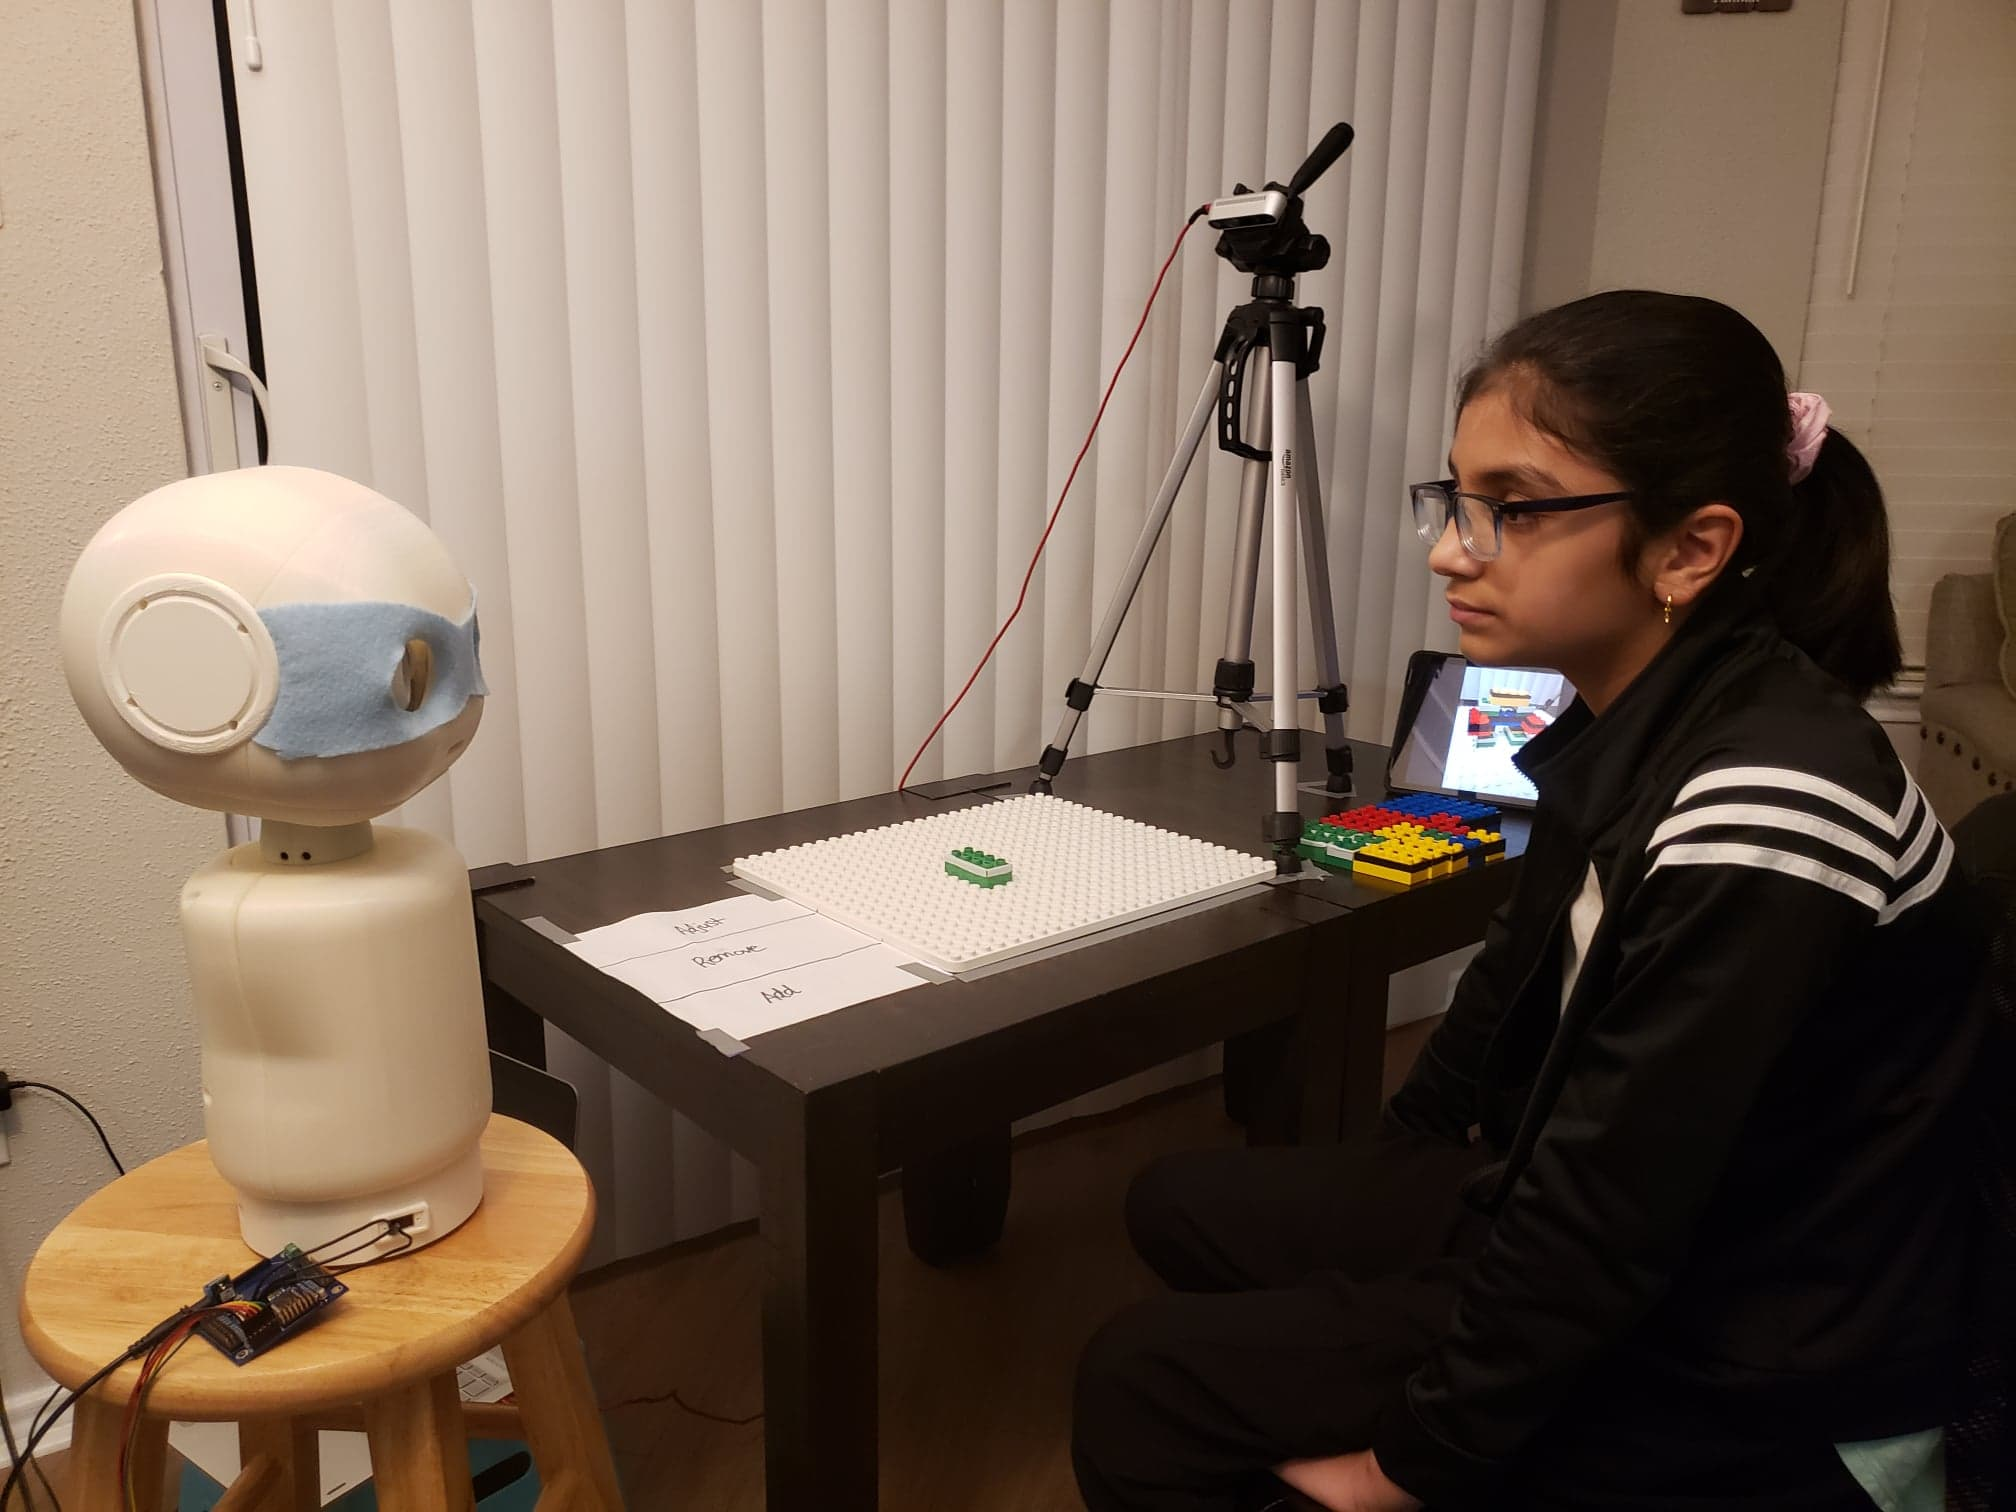
\includegraphics[width = 1\textwidth,trim={2cm 0 4cm 5cm},clip]{figures/s1.jpg}
   \caption[{System Setup}]{System Setup}
   \label{fig:fig_1-1}
\end{figure}
We contextualized our investigation into a one-on-one tutoring interaction. The setup is shown in Figure \ref{fig:fig_1-1}.  The setup consists of the following:
\begin{enumerate}
    \item Perception system: To track actions of the participant. 
    \item Intelligent Robot Tutor: Acts as a tutor to provide feedback based on actions of the participant.
    \item 3D blocks: Serves as the playground for the participant to solve designed spatial reasoning task. 
\end{enumerate}
We collected data from one participant to explore the impact of implicit and explicit feedback on self-efficacy and learning gain, and her perception of such robot tutor while working on a spatial reasoning task. Analysis of data has resulted in useful design implications for future research. We believe that this study opens an interesting research space in robot tutoring. Future studies about tradeoff between implicit and explicit feedback, effectiveness of various types of implicit feedback, its personalization and right timing for intervention etc. will follow.  \\
In the next chapter, we review prior work in field of social robotics for education, feedback practices in tutoring, and development, importance and augmentation of spatial reasoning in early ages. We give background to our study. This review is followed by a description of our system and how the exploratory study is designed along with evaluation. We then discuss our findings and their implications for future work, concluding with a summary of our contributions.


%\printbibliography[title=References]}
%\end{refsection}
%
%\begin{refsection}[myrefs.bib]
\chapter{Background}
\label{chap:two}

\sect{Spatial Reasoning}
\subsect{Definitions and Categorization}
Spatial reasoning has always been of paramount importance for human action and thought. Various verbs e.g. locating, orienting, transforming, visualizing and navigating etc. are used to indicate spatial reasoning. Thus, from navigating in 3D world to mental manipulation of objects in our surroundings before physically moving them around falls under umbrella of spatial reasoning. There is a considerable debate on the relationships among “visualization”, “visual-spatial reasoning”, and “spatial reasoning”. These terms are used interchangeably by some and some present differences. In the light of these uncertainties, Linn and Peterson (1985) \parencite{linn1986} suggested an approach to divide spatial skills into three broad categories:
\begin{enumerate}
    \item Spatial Perception: Social perception is the ability to determine spatial relationships with respect to the orientation one\textquotesingle s own body while ignoring distractions. An example test is water level task that requires participants to draw a horizontal line in titled water bottle \parencite{piaget2013growth}.
    \item Mental Rotation: Mental rotation is the ability to mentally rotate a two or three-dimensional objects rapidly and accurately. Shepard and his colleagues \parencite{cooperau1973time} \parencite{shepard1971mental} administered tasks to measure the speed of mental rotation.
    \item Spatial Visualization: Spatial visualization is the ability to perform complicated, multi-step manipulations of spatially presented information to complete a task. Such tasks may involve the similar underlying processes as in spatial perception and mental rotation but may have multiple possible correct solutions. Three dimensional block building is an example of such tasks.
\end{enumerate}
McGee \parencite{mcgee1979human} explains that there are two main factors of spatial ability:
\begin{enumerate}
    \item Spatial Visualization: Spatial visualization is the ability to imagine manipulation, rotation, twisting or inverting objects without reference to one's self. 
    \item Spatial Orientation: Spatial orientation is associated with one's ability to imagine the view of an object from different perspectives and directions. 
\end{enumerate}
In his book, Davis \parencite{davis2015spatial} uses the topological framework of spatial skills proposed by Uttal \parencite{uttal2013malleability}. The $ 2 \times 2 $ categorization scheme is based on two key dimensions of spatial reasoning: static versus dynamic and intrinsic versus extrinsic skills as summarized in figure \ref{fig:fig_1-1}. As per his analysis, the skills and tasks did not always fit into one category or the other. Skills shifted from one category to another depending on the interpretation of the task at hand or ways in which a single task is performed specially when young children's spatial reasoning is concerned. \\
Regardless of these categorization, some sort of mental imagery and manipulation is involved in spatial reasoning skills. For the scope of this study, spatial visualization component is considered and it is defined as: to be able to imagine an object from a perspective, mentally rotate it and imagine the rotated image from same or another perspective correctly to complete a complicated multi-step task.
% Figure 1-1
\begin{figure}[t] %  figure placement: here, top, bottom, or page
   \centering
%   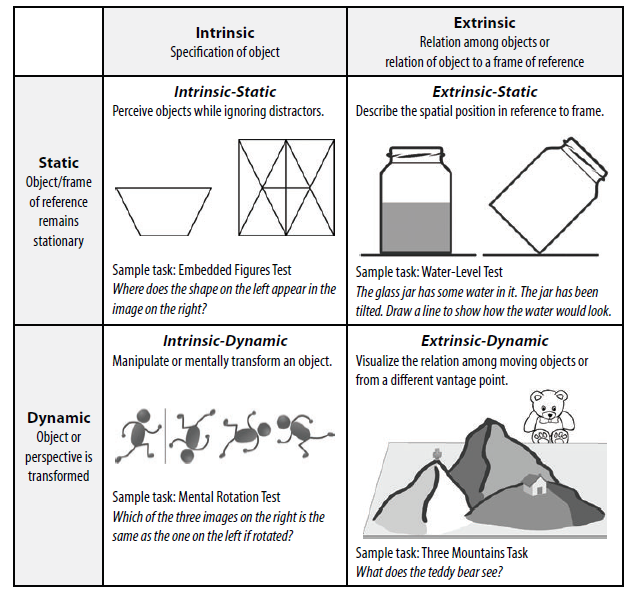
\includegraphics[width=\textwidth,height=\textheight,keepaspectratio]{fig_1-1}
   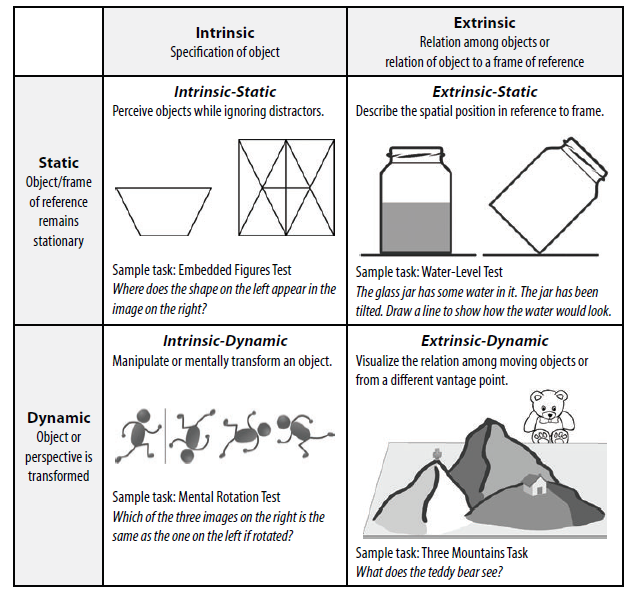
\includegraphics[scale=1]{fig_1-1}
   \caption[{2x2 topology of spatial reasoning categories}]{2x2 topology of spatial reasoning categories \parencite{davis2015spatial}}
   \label{fig:fig_2-1}
\end{figure}


\subsect{Development of Spatial Reasoning in Early Years}
Development of spatial reasoning starts in early years of human life. Different researchers have presented their theories about timeline of development of spatial reasoning skills in children \parencite{yilmaz2017development}. Piaget and Inhelder \parencite{piaget1956child} indicated that children go through three stages during this development of their cognitive spatial ability: preoperational stage, concrete operational stage and formal operational stage. They indicated that children under six years of age can locate objects with respect to themselves and are aware of topological spatial relationships. They are in preoperational stage since they understand concepts like separation, proximity and open/close. In concrete operational stage, children of ages 7-9 years develop a cognitive map with a fixed frame of reference helping them with external view and orientation such as right/left and before/behind. At age of 11, as children enter last stage i.e. formal operational stage, they understand concept of fixed positions relative to each other that assist them in understanding concepts like proportional reduction of scale, and estimating straight-line relative distances. \\
However, later around 2000, Huttenlocher and Newcombe \parencite{huttenlocher1999spatial} suggest that spatial reasoning develops even earlier, as early as at age of 6 months. Stages presented by them are summarized as follows\parencite{yilmaz2017development}: 
\begin{enumerate}
    \item Infants at age of 6 months are able to use dead reckoning skills to understand location of objects around. This helps them in keeping track of moving object's direction.
    \item At age of 12 months, babies can find hidden stimuli with help of understanding of distance.
    \item At age of 18 months, they can navigate easy routes.
    \item Using the distance information from landmarks, kids can define locations at age of 2 years. Piaget had suggested that does not happen until they are nine or ten. 
    \item Kids at age of 3 are able to use simple maps and models.
    \item If encouraged to play with maps and tools, kids can fully develop their spatial reasoning skills by the age of nine or ten. 
\end{enumerate}
Frick and Wang \parencite{frick2010round} experiments suggest that 14 month olds with some prior experience can activate mental rotation ability. Younger kids manifest the spatial reasoning skills which can be channeled by mental rotation exercises at early age to further strengthen this ability. However at this young age, children can only continue an already started rotation.\\
Research on spatial transformations has indicated complex tasks like mental paper folding task emerges at age of 5.5 years and continue to improve through early elementary school \parencite{harris2013new}. Object based spatial transformations require children to posses spatial manipulation ability of mental imagery. This occurs for kids aged between 7 and 8 years. Egocentric perspective transformations develop later at age of 8 years rather than 7, than object-based transformations \parencite{crescentini2014mental}. 

\subsect{Role of Spatial Reasoning in Mathematics}
Over 60 years ago, a report of a National Science Foundation (NSF) advisory panel, Scientific Careers, was published \parencite{super1957scientific} which emphasized on critical role of spatial ability. It was characterized as an individual difference that affected learning the advanced scientific-technical concepts for outstanding performance in STEM (science, technology, engineering and mathematics). People with exceptional spatial skills are capable of advancing the world in technology and science. Despite that this fact was established as early as 1957, spatial reasoning skills are not included in curriculum and instruction in educational settings even in STEM domains. Various studies and projects followed further solidifying the positive effect of spatial reasoning skills on success in STEM fields \parencite{wai2009spatial}. \\

There are several theories of quantitative reasoning on how spatial reasoning skills may support success in mathematics. Dehaene and his colleagues suggests that quantitative reasoning comprises of two core systems of numbers which tap different neural networks in the human brain: one being approximate and non-symbolic and the other is precise and symbolic. It is suggested that the first core shares neural activity with spatial reasoning skills and the second core is more associated with exact counting and symbolic mathematical operations \parencite{feigenson2004core}. As early schooling results in the two core systems of numbers merging, spatial skills' impact on mathematics achievement via the second symbolic system of number will increase significantly. Symbolic and non-symbolic numerical thinking will mutually enhance one and other as these are taught over time. \parencite{piazza2013education}. Existing evidence suggests that the spatial skills, if polished in early elementary school curriculum, will provide a strong foundation for mathematics achievement in elementary school and beyond. \\
Various studies imply that in elementary school students, spatial skills are known to support understanding of geometry \parencite{clements1997development},  word problem solving and application of more complex and complicated computation strategies\parencite{manger1998effects} , especially in girls \parencite{dearing2012young}. Longitudinal studies have also shown that early spatial skills predict later success in mathematics. For instance, spatial reasoning skills measured in first-grade girls are crucial predictors of fifth-grade analytical math reasoning.  First-grade assessments included spatial skills, verbal skills, addition/subtraction skills, and frequency of choice of a decomposition or retrieval strategy on the addition/subtraction problems. In fifth grade, girls were given an arithmetic fluency test, a mental rotation spatial task, and a numeric and algebra math reasoning test \parencite{casey2017girls}. Similarly, spatial visualization predicted as early as in kindergarten reflects arithmetic skills in third graders. Linguistic and spatial skills can improve arithmetic development by enhancing children's number‐related knowledge \parencite{zhang2014linguistic}. Even at early ages, both mental rotation and spatial visualization skills have depicted associations with numeric operations and  addition and subtraction computational skills in grade 1,2,3 and even in kindergarten. A 32-week-teacher-led spatial reasoning intervention in K-2 classrooms highlighted the importance of assisting development of spatial visualization in young kids as part of early mathematics instruction \parencite{Hawes2017}. Another longitudinal study investigated the development of spatial reasoning skills in 304 elementary school children as they progressed from grade 2 to 4 which outlines effects of socioeconomic status, verbal working memory and gender \parencite{carr2018development}. \\
To summarize, spatial reasoning skills contribute positively to development of mathematical understanding at early ages and are pertinent to achievements in STEM fields later on. Thus, such skills need to be included in elementary school curriculum to ensure higher success rate of individuals in engineering and mathematics. 

\subsect{Ways to Augment Spatial Reasoning}
Spatial reasoning can be augmented using various activities and games. Following are some ways suggested to improve spatial skills:
\begin{enumerate}
    \item Use spatial language and gestures in everyday instructions: Using spatial language such as inside, outside, left, right, behind, on top of etc. assists babies in learning spatial relations better \parencite{casasola2008development}. For example sentences to describe scenes: The car is across the street under the tree. Asking kids to repeat after you helps further. Hand-gestures along with spatial language can help kids learn better \parencite{singer2005children}
    \item Teach how to visualize using mind's eye: Visualization is an essential tool for spatial learning. If kids are instructed to visualize a problem while solving it, they would perform much better. For instance, in an experiment, when a ball is dropped even through a twisted tube, preschooler would tend to think it falls right under. But when young kids are distracted from their gravity bias by instructing them to visualize the path of the ball, more students get the right answer \parencite{joh2011imagining}.
    \item Two-dimensional Puzzles and other activities: Various puzzles and matching games can be used to enhance spatial reasoning skills of kids. For instance, tangram, an ancient Chinese puzzle that consists of 7 pieces and can be rearranged into many different shape can help increase spatial skills of students \parencite{siew2013facilitating}.  Similarly, jigsaw puzzle, origami, paper folding, and other open-ended puzzles can help augment spatial visualization skills of kids as these require mental manipulation of various shapes. 
    \item Three-dimensional block play: Building structures and objects with 3D blocks e.g. Lego\textsuperscript\textregistered{} \parencite{wolfgang2003advanced} and wooden blocks can significantly increase children's ability to manipulate things mentally. Giving them a structure to build will expand their knowledge of spatial visualization. Block play is important in early years in helping kids understand spatial reasoning skills which are important for later STEM learning. When kids are prompted and asked questions about their block play structures by teachers or helpers, it grows their use of spatial language as well which is related to increase in spatial reasoning \parencite{pruden2011children} and can play an important role in scaffolding children’s building of more complex structures \parencite{kersh2008research}. A planned block play program similar to Carol Stephenson can help greatly in developing spatial reasoning skills through building complex block structures \parencite{tepylo2015developmental}. A study examining children's puzzle play \parencite{levine2012early} shows that it predicts children's later performance on a spatial transformation task. It also discusses how early puzzle play varies across children and engagement is associated with demographic variables as well as levels of parent language input.
    %% https://www.parentingforbrain.com/visual-spatial-reasoning-skills-stem/#improve
\end{enumerate}
For the sake of this research, we have identified 3D block building as the way to augment spatial visualization that we experiment with in our system since 3D block building tasks is a multi-step complex process that involves spatial visualization, mental rotation and perspective taking skills.


% New section
\sect{Child-Robot-Tutoring}
Social robots have made their way in educational setting for children in recent years. Research community has been focused on various aspects of social robots in education. Benefits of social robots, technical challenges for building robot tutors, their efficacy, impact of their appearance, role and their behaviour has been vastly studied \parencite{belpaeme2018social}. Application of social robotics in education has become popular because of availability of robust platforms, mature technology to the point that meaningful interactions using language and nonverbal behaviour are possible, and the established fact that embodiment results in higher learning gains in educational settings. In various educational settings embodiment of a robot plays an important role on improving the children's performance, engagement and motivation \parencite{kose2015effect} \parencite{kennedy2015comparing}. Many aspects of child-robot-tutoring has been investigates such as building models of student knowledge \parencite{spaulding2016affect}, evaluating different teaching and instruction paradigms \parencite{hood2015children}, personalizing content for each child \parencite{gordon2016affective} and determining when and how to provide specific kind of assistance and hints \parencite{ramachandran2016shaping}. Much of work in which robot is used as a tutor focuses on one-to-one interactions because these offer the greatest potential for personalization \parencite{belpaeme2018social} \parencite{ramachandran2019personalized}. Most of the research is limited to teaching languages \parencite{gordon2016affective} and solving mathematical problems \parencite{ramachandran2019personalized}. 

%%scaffolding 

\subsect{Child-Robot-Tutoring and Spatial Reasoning}
Spatial reasoning is rather unexplored in one-to-one child-robot-tutoring. Reasons can be complexity of interaction, lack of ways to track performance and measure learning gains during complex tasks and difficulty in providing appropriate feedback. However, over the past two decades computer-supported educational tools are being used in learning of spatial skills particularly reflected in geometry e.g. Edwards created a computer environment that enabled kids to learn introductory geometric transformations\parencite{edwards1991children}. GeoCAL \parencite{chang2007developing}, a multimedia learning software based on van Hiele's theory of geometric thinking \parencite{chang2007developing} comprising of several games such as jigsaw puzzles, shape tracer and stamping, has notable learning effects on geometric thinking (visual association, description and abstraction). \\
However, models designed to improve spatial ability in 2D world by using Web-based virtual environment \parencite{rafi2005improving}  may not work at all in 3D world because of over-simplification of the environment. Therefore, Keren et al. 
\parencite{keren2012kindergarten} suggested that spatial cognition models should at least be partially embodied and assistive robots can serve the purpose in developing children's visual-spatial and motor perception. They use assistive robots for groups (2-3 kids) of kindergarten students to promote their geometrical thinking which is one aspect of spatial cognition. The activity for this study is modification of their previous research i.e. Nao (the robot) singing the Hebrew version of song, "Head, Shoulders, Knees and Toes" while demonstrating the movements and invited kids to do some movements \parencite{fridin2014robotics}. In this study, robot asks to recognize basic shapes on screen and distinguish between upper and lower parts of its body and are asked to find and push relevant buttons. \\
To summarize, development of spatial reasoning specially spatial visualization skills in 3D environment using educational social robotics is limited and rather unexplored. Thus, in this exploratory study we focus on providing a learning platform comprising of a robot tutor to help learn spatial visualization skills using 3D Lego\textsuperscript\textregistered{} block building. We track the performance of children and assist them in completing a Lego\textsuperscript\textregistered{} structure building task in one-to-one child-robot-tutoring session.     

\sect{Feedback Strategies}
Good feedback practices by tutors in one-on-one sessions are essential for self-regulated learning. Good feedback practice is broadly defined as something that reinforces the student's capability to self-regulate their own performance. Self-efficacy in turn has positive effects on not only achievement, but also motivational variables such as engagement, effort, persistence etc. \parencite{narciss2004impact}. For designing a good feedback practice, one needs to consider many factors. One of many principles to think about design and evaluation of self-created feedback procedures, is that feedback can be provided by a teacher, peer or tutor. Seven principles to think about design and evaluation of self-created feedback procedures are described below \parencite{nicol2006formative}: 
Good feedback practice: 
\begin{enumerate}
    \item helps clarify what good performance is (goals, criteria, expected standards)
    \item facilitates the development of self-assessment (reflection) in learning
    \item delivers high quality information to students about their learning
    \item encourages teacher and peer dialogue around learning;
    \item  encourages positive motivational beliefs and self-esteem
    \item provides opportunities to close the gap between current and desired performance
    \item  provides information to teachers that can be used to help shape teaching
\end{enumerate}
Informative tutoring feedback provides useful information strategically for task completion rather than offering complete solution. Interactive-Tutoring-Feedback (ITF) refers to feedback components to guide the student toward successful task completion. Narciss has proposed the ITF model that encapsulated the state of the art in developing feedback strategies for interactive learning tasks \parencite{narciss2005informatives} \parencite{narciss2008feedback} \parencite{narciss2013designing}. As per this ITF model, a feedback strategy is defined as a coordinated plan integrating clear and decisive statements specifying at least the following aspects of a learning process with feedback \parencite{narciss2012feedback}:
\begin{enumerate}
    \item \textit{scope and function}: what goals or purposes the feedback serves.
    \item \textit{content}: what information is given through the feedback.
    \item \textit{presentation}: in which form and modes the feedback content is given.
    \item \textit{conditions}: under which situational or individual conditions the feedback is provided.
    \item \textit{timing and schedule}: which event within the learning process trigger feedback statements. 
\end{enumerate}
This definition enables a wide range of possibilities when it comes to designing feedback strategies. Feedback comes in various forms and modes i.e. immediate vs. delayed feedback timing, single-try vs multiple-try, adaptive vs non-adaptive and implicit vs explicit feedback \parencite{narciss2008feedback}. In human-human-interactions, experienced tutors tend to provide indirect feedback to bring the attention of students to an error rather than giving corrective explicit feedback \parencite{lepper1990self}. Indirect corrective feedback is argued to address some of weakness of direct corrective feedback (CF) (e.g. no explanation to why the correction is needed), as indirect CF engages learners to analyze their own work and figure out and correct their mistakes Expert tutors also employ subtle techniques like delaying affirmation or expressing short hesitation when student inquires if he is doing alright, thus, hinting him about a mistake in the current step \parencite{fox1991cognitive}. There are other strategies like asking a leading question or subtly suggesting the student to redirect. Such strategies are enlisted in table \ref{tab:tab_2-1}. On the other hand, it is argued that providing only implicit feedback can be detrimental. If a student spends too much time guessing for a solution or redirecting himself, it would be difficult for him to trace the path he took to solution \parencite{lewis1985discrimination}. Therefore, the tutoring strategy should be a trade-off between implicit and explicit feedback to allow room for the student to explore and learn from his mistakes, yet not be confused or stuck at an impasse. 

\begin{longtable}{ | m{30em} | m{2cm}|  } 
\hline
\textbf{Feedback Strategy} & \textbf{Reference}  \\ 
\hline
1. Draw student’s attention to an error and provide second chance & \parencite{lepper1990self}  \\ 
\hline
2. Frequent feedback: Brief agreement with each step (e.g. Mhm, Right etc. when student is thinking out loud looking for agreement) or a short hesitation (often less than 1 sec) in responding with an “okay” indicating to students to assume that something was amiss with the current step & page 9,10 of \parencite{fox1991cognitive}  \\ 
\hline
3. Asking a leading question/ giving clues & \parencite{fox1991cognitive}\\
\hline
4. Asking a leading question/ giving clues.  Wait for student to complete your utterance, if student fails, complete it. Both work to avert a wrong solution & \parencite{lepper1990self}\\
\hline
5. Procedural hints and explanations: procedural hints point out appropriate strategy or mention key aspect of underlying concepts (e.g,. \emph{When expanding a fraction, one alters the numerator and denominator equally}). While procedural explanations provide more details about how to put this procedure into practice. (e.g., \emph{When expanding a fraction, one alters the numerator and denominator equally. To do this, multiply the numerator and denominator by the same number.}). & \parencite{narciss2014exploring}\\
\hline
6. Conceptual hints and explanations: focus on conceptual knowledge important for solving the target problem e.g., conceptual hint: \emph{When expanding a fraction, its value must not change.} and conceptual explanation: \emph{When expanding a fraction, its value must not change. While expanding, the denominator increases, that means the partitioning becomes more fine-grained. But since the value of the whole fraction does not change, the numerator has to be altered in the same way}. Conceptual explanations provide additional information about relevancy of the concepts to the given problem. & \parencite{narciss2014exploring} \\
\hline
7. Feedback consists of following components: & \parencite{parvez2008individualizing}\\
a. Definition: verbally introduce definitions of domain concepts e.g. \emph{Attributes are characteristics of an object that persist through the life of the object.}. & \\
b. Example: give an illustration of given concept e.g. \emph{Attributes of a car might be its color, model, make etc.} & \\
c. Question: ask a question for clarity of learner e.g. \emph{Why did you set the data type for money to string?} & \\
d. Scaffold: prompts the learner who might be lost towards a correct solution by pointing in right direction e.g. \emph{Use the tutorial to learn about datatypes.} & \\
e. Picture: contains images, animation or video to visually explain a concept. & \\
f. Relationships: provides information to help learner understand how a concept fits into the overall problem solving activity. & \\
g. Application: shows application of a concept e.g. a learner might know definition of a constructor but might not know that a class could have multiple constructors. & \\
h. Exercise: supports active learning through hands-on activities or by applying a concept. It is more like a tutorial mode. & \\
\hline
8. Corrective feedback have been classified into two groups for second language teaching: & \parencite{ferreira2007study} \\
a. Giving-Answer Strategies (GAS): when teacher directly gives the target form or shows the location of student's error. These includes: repetition, recast, explicit correction and giving answer. &\\
b. Prompting-Answer Strategies (PAS): when teacher pushes students to notice their error and correct it themselves. These include: Meta-linguistic cues (teacher provides information or asks questions regarding the correctness of the student's utterance), clarification requests and elicitation(allowing student to complete teacher's utterance, by asking student to reformulate the utterance etc.). & \\
\hline
\caption[Feedback strategies from literature]{}
\label{tab:tab_2-1}

\end{longtable}

Kleij et al. \parencite{van2015effects} present a meta-analysis of effects of feedback on  student's learning outcomes in computer-based learning environments. They deduce that elaborated feedback is particularly more effective than feedback regarding correctness of answer and providing correct answer, specially in mathematics. The results suggested that immediate feedback is better for lower order learning than delayed feedback, whereas delayed feedback is more effective for high order learning. In literature, there are contradicting results about effectiveness of immediate and delayed feedback. It seems to be task dependent. Thus, for sake of this exploratory study we focus on providing direct/explicit or indirect/implicit feedback as soon as a mistake is made. We also provide confirmations on correct actions of user.  





%\printbibliography[title={References}]
%\end{refsection}
%
%\begin{refsection}[myrefs.bib]
\chapter{System Overview}
\label{chap:three}
The system is set up as a play area where a user tries to replicate a 3D Lego\textsuperscript\textregistered{} structure in presence of a robot tutor which provides requisite feedback towards completion of the task. The system, as shown in figure \ref{fig:fig_1-1}, consists of three modules:
\begin{enumerate}
    \item Perception: Tracks the play area using color + depth (RGB-D) camera stream to detect errors.
    \item Feedback: Robot provides selected feedback based on errors detected. 
    \item Robot Behaviour: Behavioural actions displayed by the robot that makes it life-like. 
\end{enumerate}

\sect{Perception}
Perception module tracks the actions of user while building the given 3D structure in the play area. Output of this module is mistakes made by users. This module has various aspects such as detection of RGB-D data, detection of different types of Lego\textsuperscript\textregistered{} blocks, actions taken by user to manipulate the structure, creating and storing a model of structure and comparing it to target structure to look for mistakes made by user. These aspects are explained below in detail:

\subsect{Setup}
The system consists of a RealSense\textsuperscript\textregistered{}  d435i color + depth (RGB-D) camera mounted on a stand to the right of table surface looking at the playground from right side while the user sits in front of table as shown in figure \ref{fig:fig_1-1}. The camera looks obliquely down on the table surface. On the left side of the table, there is a robot named Maki who acts as a tutor. A set of $2 \times 2$ and $2 \times 4$ Lego\textsuperscript\textregistered{} blocks in 4 basic colors (red, blue, green and yellow) are placed on the table within the reach of user. The table surface has four demarcated regions - \textit{Play area, Add box, Remove box and Adjust box}. The last three areas are used as control boxes for the users to define their actions. This setup is inspired from research by Gupta and colleagues \parencite{gupta2012duplotrack}. A base plate for blocks is placed in play area to fix the assembly of Lego\textsuperscript\textregistered{} blocks. The function of each control box is defined as under:
\begin{enumerate}
    \item Add box: If user intends to add a block to assembly, he would place the block in the \emph{add box} for a couple of seconds before moving it to play area which will indicate the tracking system to look for a new block of given shape and color in the play area. 
    \item Remove box: If user intends to remove a block from assembly, he would remove the block from play area and place it in the \emph{remove box} before placing it on side of a table, which will indicate the tracking system to look for a block of given shape and color that has been removed from the play area to update the model.
    \item Adjust box: If user intends to adjust a block (change it's position) in the assembly, he would remove the block from play area and place it in the \emph{adjust box} and then move it back to play area as per his desire. This will indicate the tracking system to look for and remove the block of given shape and color from the assembly once a block is detected in \emph{adjust box} and then start looking for the same block in play area to add it to a new location. 
\end{enumerate}

\subsect{Different Modes}
The main goal of system is to track user's performance towards completion of a target 3D structure and flag the mistakes made by user during the process. To achieve that system must compare the assembly to the target structure during the task. To do so, the tracking system must learn the target structure first. Thus, to comply with the requirements, we propose that the system operates in two modes:
\begin{enumerate}
    \item Learning Mode: In learning mode, the experimenter (or teacher, supervisor, parent o guardian of the user) builds the required 3D structure using add, remove and adjust commands. The tracking system stores the constructed 3D structure as a target structure in a file. The representation of play area, block models and 3D structure is explained in section below. In short, the system learns the structure from demonstration by human expert in learning mode. 
    \item Teaching Mode: In teaching mode, the system tracks the assembly of 3D structure by the user (a child) and compares each action taken by user with the target structure and flags any mistake made. It compares the current structure with the target structure on every user action and evaluate the deviations from each possible correct action since there can be multiple correct actions at every step. If the user action does not coincide fully with any of the possible correct actions, an error is flagged. In short, the system is teaching the user a learned structure in this mode.
\end{enumerate}

\subsect{Representation of Play Area and Blocks}
For tracking the model and inferring updates, the system needs some sort of representation for the assembly model. We assume that the model resides in a voxelized space \parencite{gupta2012duplotrack} where each voxel is equal to $1 \times 1$ Lego\textsuperscript\textregistered{} block. Thus, the model is made of $2 \times 2$ block  that occupies 4 voxels and $2 \times 4$  blocks that occupy 8 voxels. Following information is maintained for the model which is coded as a class (\textbf{Assembly\_Graph}) in python. For learning and teaching modes, there are slight changes in the class attributes and functions which will be discussed as needed. 
\begin{enumerate}
    \item \textbf{.block\_dict}: A dictionary of structure type \emph{Block} (class created in python) where each block has following attributes:
    \begin{enumerate}
        \item \textbf{.xy}: list of voxels that the block is occupying. x and y coordinates represent the voxel as (x,y). The first block , called the reference block, is fixed in the play area and its top left corner (from camera's viewpoint) is assigned the value of (0,0) where x increases towards right and y increases downwards. Voxel (0,0) is circled in figure \ref{fig:fig_3-2} as the green rectangular block is the reference block and it has \\
        $\textbf{.xy} = [(0,0), (1,0), (2,0), (3,0), (0,1), (1,1), (2,1), (3,1)]$.  The workspace is represented as a grid of voxels with (0,0) at the top left corner of the reference block. \textbf{.xy} of all other blocks is calculated with reference to (0,0) voxel. 
        \item \textbf{.z}: \textbf{.z} is level from base. Base is at zero level so first layer of blocks will be at level 1 i.e. $\textbf{.z} = 1$ e.g. in figure \ref{fig:fig_3-2} green and red blocks are at \textbf{.z} $=1$ and yellow block is at \textbf{.z} $=2$. \textbf{.z} is obtained from depth data corresponding to the center pixel of the block. The value is converted into integer levels e.g. 1,2,3 etc. after gathering some data points in the play area. Error correction in depth values may be needed since the camera is mounted at an angle and depth values for same level varies across the y-axis. Thus, a linear line is fitted on the gathered data points where error in depth varies with y position of the center pixel. This reduces the error in measurement of \textbf{.z} to great extend but sometimes in higher levels the error still exists and it always mistakenly return higher level than required e.g. at level 6, system assigns value of 7 or 8 instead etc. To further reduce this error, we use the information we already have in the model. Consider the above example: if we get level 7 instead of level 6 for new block, while evaluating \textbf{.overlap} and \textbf{.overlap\_dict} (see below), if we get empty dictionary (means no block under the new block), we decrease \textbf{.z} by 1 since it is impossible for a new block to not be connected to any block underneath it if $\textbf{.z} > 1$. It checks \textbf{.overlap\_dict} again and continues subtracting 1 from \textbf{.z} till there is at least one block or base of play area underneath the new block.
        \item \textbf{.angle}: \textbf{.angle} can have only two values: 0 or 90 degrees since the base of play area is fixed and blocks can only be placed at two angles. Also, it only matters if it is a $2 \times 4$ block. So, \textbf{.angle} is assigned a value of 0 when 4 voxels are along y-axis and 2 voxels are along x-axis and a value of 90 (90 degrees rotation) otherwise. For a $2 \times 2$ block it is always 0.  As shown in figure \ref{fig:fig_3-2}, the green and red blocks are at an angle of 90 degrees while yellow has angle of 0 degrees.
        \item \textbf{.shape}: \textbf{.shape} can have one of two values, either 1 or 2:  1 for $2 \times 2$ block and 2 for $2 \times 4$ block.
        \item \textbf{.color}: \textbf{.color} can have one of four values: 1 for red color, 2 for blue, 3 for green and 4 for yellow.
        \item \textbf{.idx}: \textbf{.idx} is a unique ID assigned to each block that is a part of assembly. 
        \item \textbf{.overlap}: \textbf{.overlap} is a Boolean variable which is true when the block is connected to another block below it, in the assembly apart from base of play area.
        \item \textbf{.overlap\_dict}: \textbf{.overlap\_dict} is a python dictionary that contains information of all the blocks connected under the new block. Keys in this dictionary are the \textbf{.idx}s of the connected blocks and associated with those keys are \textbf{.xy} voxels of the respective blocks that overlap with the new block. For instance, as shown in figure \ref{fig:fig_3-2}, the yellow block(\textbf{.idx} $ = 3$) will have \textbf{.overlap\_dict}  $= \{1:[(1,1),(2,1)], 2:[(1,4),(2,4)]\}$ since it overlaps with blocks of \textbf{.idx}s 1(green block) and 2(red block) whereas blocks 1 and 2 will have empty \textbf{.overlap\_dict} since there is only base underneath those.
    \end{enumerate}
    \item \textbf{.graph\_dict}: It is a dictionary that stores connections of each block with other blocks directly connected on top of it using their \textbf{.idx}. For instance, if the target structure has only three blocks and block with \textbf{.idx} 3 is connected on top of blocks with \textbf{.idx} 1 and 2(see figure \ref{fig:fig_3-2}), \textbf{graph\_dict} will be: $\{1: [3], 2: [3], 3:[\:]\}$. Just by looking at this structure we can tell that only block 3 can be removed in the next step and not 1 and 2 since removing those would require removing block 3 first. This dictionary helps us keep track of removable blocks at any step. 
    \item \textbf{.graph\_dict2}: It is another dictionary that stores connections of each block with other blocks directly connected below it using their idx. This dictionary is useful when we need to compare structures in teaching mode. At each step, it is used to find out all possible correct actions given the target structure. For instance, if the target structure has only three blocks and block with \textbf{.idx} 3 is connected on top of blocks with \textbf{.idx} 1 and 2 (see figure \ref{fig:fig_3-2}, \textbf{.graph\_dict} will be: $\{1: [\:], 2: [\:], 3:[1,2]\}$.  If in the current structure, during teaching mode, the user has only placed block 1 correctly.Looking at the example dictionary we can tell, the only next correct action is to add a block similar to block 2 since it does not have any block under it, which is not already added. Just by looking at this dictionary, we can tell that 3 can only be added after both 1 and 2 have been added in the assembly since 3 has to be on top of 1 and 2. Thus, this dictionary helps us identify all the possible correct actions at any step.
    \item \textbf{.pub}: \textbf{.pub} is only used in the teaching mode. It is a ROS publisher for message type \emph{String} that publishes the feedback statement for robot to provide to the user when a mistake is made. 
\end{enumerate}
\begin{figure}[h]
   \centering
%   \includegraphics[width=\textwidth,height=\textheight,keepaspectratio]{fig_3-4}
   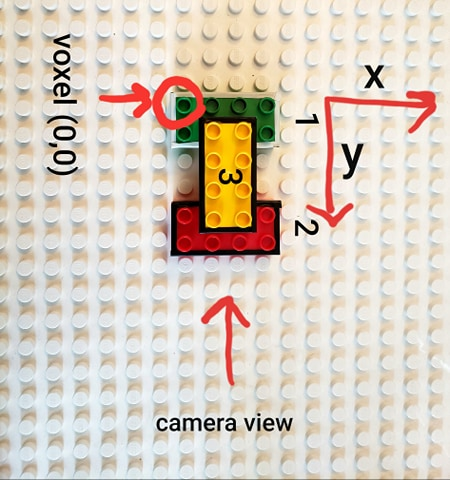
\includegraphics[width = 0.8\textwidth]{figures/voxel_3objs.jpg}
   \caption[{Attributes of \emph{Assembly\_Graph} and \emph{Block} explained}]{Attributes of \emph{Assembly\_Graph} and \emph{Block} explained: The reference voxel (0,0) is circled in red. Green block has .idx $=1$, red block has .idx $= 2$ and yellow block has .idx $= 3$. Green and red blocks are at 90 degrees angle and yellow is at 0 degrees. Green and red blocks need to be placed before yellow block. Yellow block is the only block that can be removed in the next action.}
   \label{fig:fig_3-2}
\end{figure}

For teaching mode, class \textbf{Assembly\_Graph}, has an extra attribute of type \textbf{Assembly\_Graph} to pass the target dictionary that is saved in learning mode. Using these attributes various functions are defined within the class to add and remove blocks, save and load the model, display the model and compare the models to flag errors. Feedback selection and passing the feedback statement to robot is done using functions within this class as well. 

\subsect{Processing Pipeline}
Figure \ref{fig:fig_3-3} shows the work flow of the system for both modes. The RealSense\textsuperscript\textregistered{} d435i camera captures and provides a continuous RGB-D images stream. First of all, the reference block is added to the model giving (0,0) coordinates for \textbf{.xy} of class \emph{Block} as described above. Once that is done successfully, the system scans for control command in three control boxes: add, remove and adjust. As soon as a block is detected in one of the control boxes, the system processes the play area for requisite action and updates the model accordingly. If system is in learning mode, on completion of required action, the system again scans for new action and the cycle continues till program is exited. If system is in teaching mode, on completion of requested action, the system compares the current action with all possible correct actions (comparison is made on add and adjust commands and not on remove command) and forwards the errors with respect to every possible correct action to the feedback module. The feedback module chooses a message based on errors and feedback strategy which is published for the robot to convey to the user. Once this action is completed, system starts scanning the control boxes again for next action request. The system exists when the current model is same as target model. In the following sections, we describe details of how each step in the workflow is accomplished. 
% Figure 3-3
\begin{figure}[h]
    \begin{subfigure}{1\textwidth}
       \centering
    %   \includegraphics[width=\textwidth,height=\textheight,keepaspectratio]{fig_3-3}
       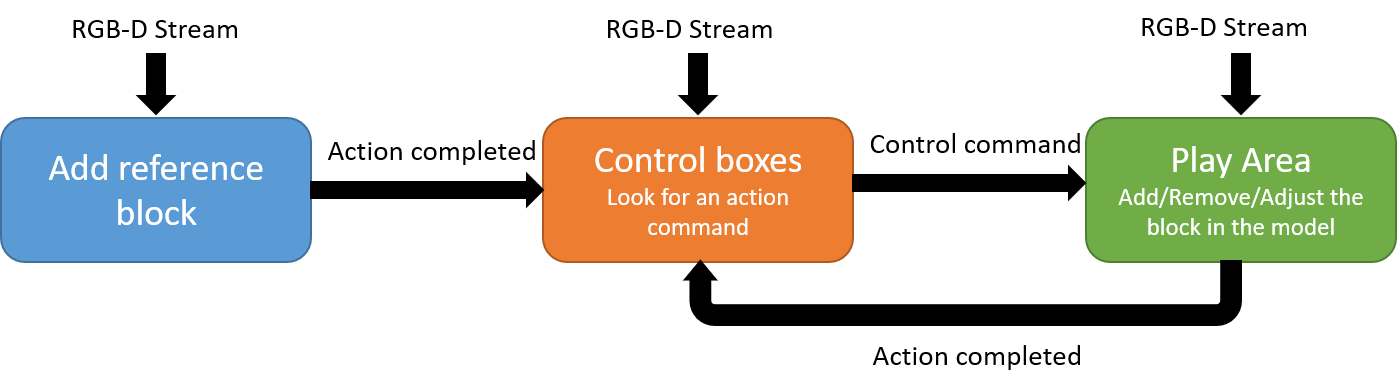
\includegraphics[width=1\linewidth]{figures/learning_mode.png}
      
       \caption[{Learning mode}]{ \label{fig:fig_3-3a}}
    \end{subfigure}
    \begin{subfigure}{1\textwidth}
       \centering
    %   \includegraphics[width=\textwidth,height=\textheight,keepaspectratio]{fig_3-3}
       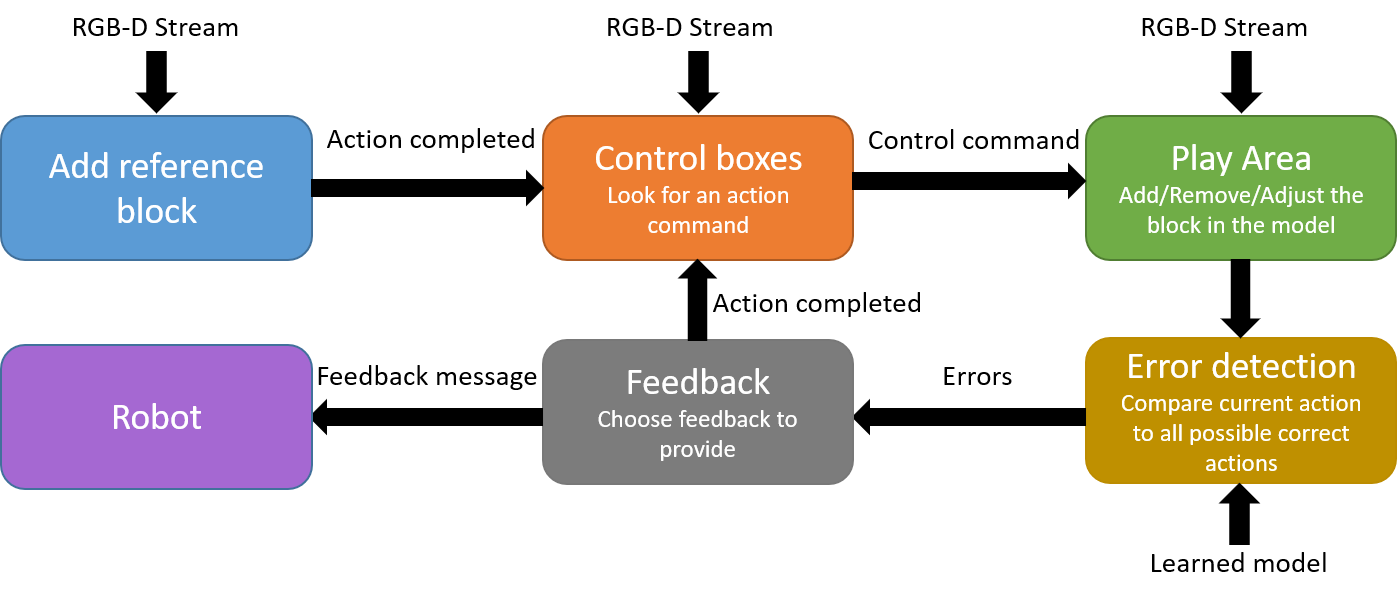
\includegraphics[width=1\linewidth]{figures/teaching_mode.png}
      
       \caption[{Teaching mode}]{ \label{fig:fig_3-3b}}
    \end{subfigure}
    \caption[{Processing pipeline}]{Processing pipeline for perception module (a) for learning mode (b) for teaching mode}
   \label{fig:fig_3-3}
\end{figure}
\subsect{Scanning Control Boxes}
The continuous RGB image stream is divided into 4 fixed regions: add box, remove box, adjust box and play area. The add, remove and adjust boxes are scanned for next command after reference block is added. The RGB image from each box is segmented using Hue, Saturation, and Value (HSV) based color segmentation to create a binary mask for each of the four colors (red, green, blue and yellow). Bounding rectangle is found for largest contour in the mask by using builtin functions of openCV (findContous(arguments), max(arguments) and boundingRect(arguments)). If a bounding rectangle is found for same color in same control box for 50 consecutive frames, it is considered a control command. The color and shape (assigned by looking at width to height ratio of the bounding rectangle) of the new block is noted, the respective command (add, remove or adjust) is activated and system starts scanning play area.
\subsect{Scanning Play Area}
RGB-D continuous stream is scanned for new action as per the control command. For  add action, first of all, the RGB image is segmented using HSV based color segmentation to create binary mask of color of new block (color is known from control command). Now, this mask is compared with masks from previous frames and if there is no change in the mask for n of consecutive frames (n= 50 for our system), all contours whose bounding boxes have width of more than m pixels (m = 15 for our system) and have the same shape as indicated by control box are considered as \emph{possible additions}. The x and y pixel coordinates of the center of each bounding box is used to get depth (z) from the corresponding depth data. If the block is $2 \times 4$ block, angle is calculated for each possible addition using ratio of width to height of the bounding box. Next, all the \emph{possible additions} are compared with the existing blocks in the model (x,y,z, shape, color and angle). The contours that coincide with existing blocks in the model are discarded thus leaving us with the contour of new block. This block is then added to the model by passing its attributes (x,y,z,shape, color, angle). The system keeps scanning the play area for new block till a block is added in the model. Once the block is added, the system generates a flag indicating that the add action is completed. For learning mode, each time new block is added \textbf{.idx} is counted up. For teaching mode, if the new block added in the current model matches one of the blocks in target model, \textbf{.idx} of the new block in the current model is assigned the same value as in target model otherwise it is assigned a much higher value e.g. 21, 22, 23. This makes comparison of two models efficient and easy. \\
For remove action, mask of known color is created using HSV based color segmentation and is compared with previous frames till there is no change for n consecutive frames (n = 50 for our system). Contours with bounding boxes are calculated. From the model, using a function \textbf{.removable\_blocks()}, we can get the \textbf{.idx} of all the blocks that can be removed from the current dictionary. We can also get the \textbf{.idx} of blocks in the model of the shape and color associated with the remove command. Intersection of these two lists, will give us \emph{possible removable blocks} i.e. the \textbf{.idx} of the blocks that are removable and of given specifications from remove command. If it is only one block that lies at intersection of these two lists, we remove that block from the model. If there are multiple blocks that can be removed, we look at the bounding boxes of contours of known shape and check which blocks from the model are still in the play area by comparing x, y, z and angle of the contours to the blocks in the model. Discard the \textbf{.idx} of these blocks from \emph{possible removable blocks} as these are still present in the play area. There should only be one block left behind in list of \emph{possible removable blocks}, which is the one that has been removed from the play area and placed in the remove box. System generates a flag indicating that the action is completed successfully when the block is removed from the model. Remove action is same for both learning and teaching mode. \\
For adjust action, remove action is completed followed by add action for the block detected in adjust box. System generates a flag on completion of action and starts scanning for next action. 
\subsect{Types of Errors Detected}
Following types of errors are detected for new block to be added in comparison to all possible correct blocks and passed to feedback module:
\begin{enumerate}
    \item Shape: The shape of new block is different from the possible correct block.
    \item Color: The color of new block is different from the possible correct block.
    \item Orientation: The orientation of new block is different from the possible correct block.
    \item Level: The \textbf{.z} (z-level) of new block is different from the possible correct block.
    \item Position: The center of new block is different from the possible correct block.
\end{enumerate}


% Figure 3-6
\begin{figure}[H]
    \begin{subfigure}{0.5\textwidth}
       \centering
    %   \includegraphics[width=\textwidth,height=\textheight,keepaspectratio]{fig_3-3}
       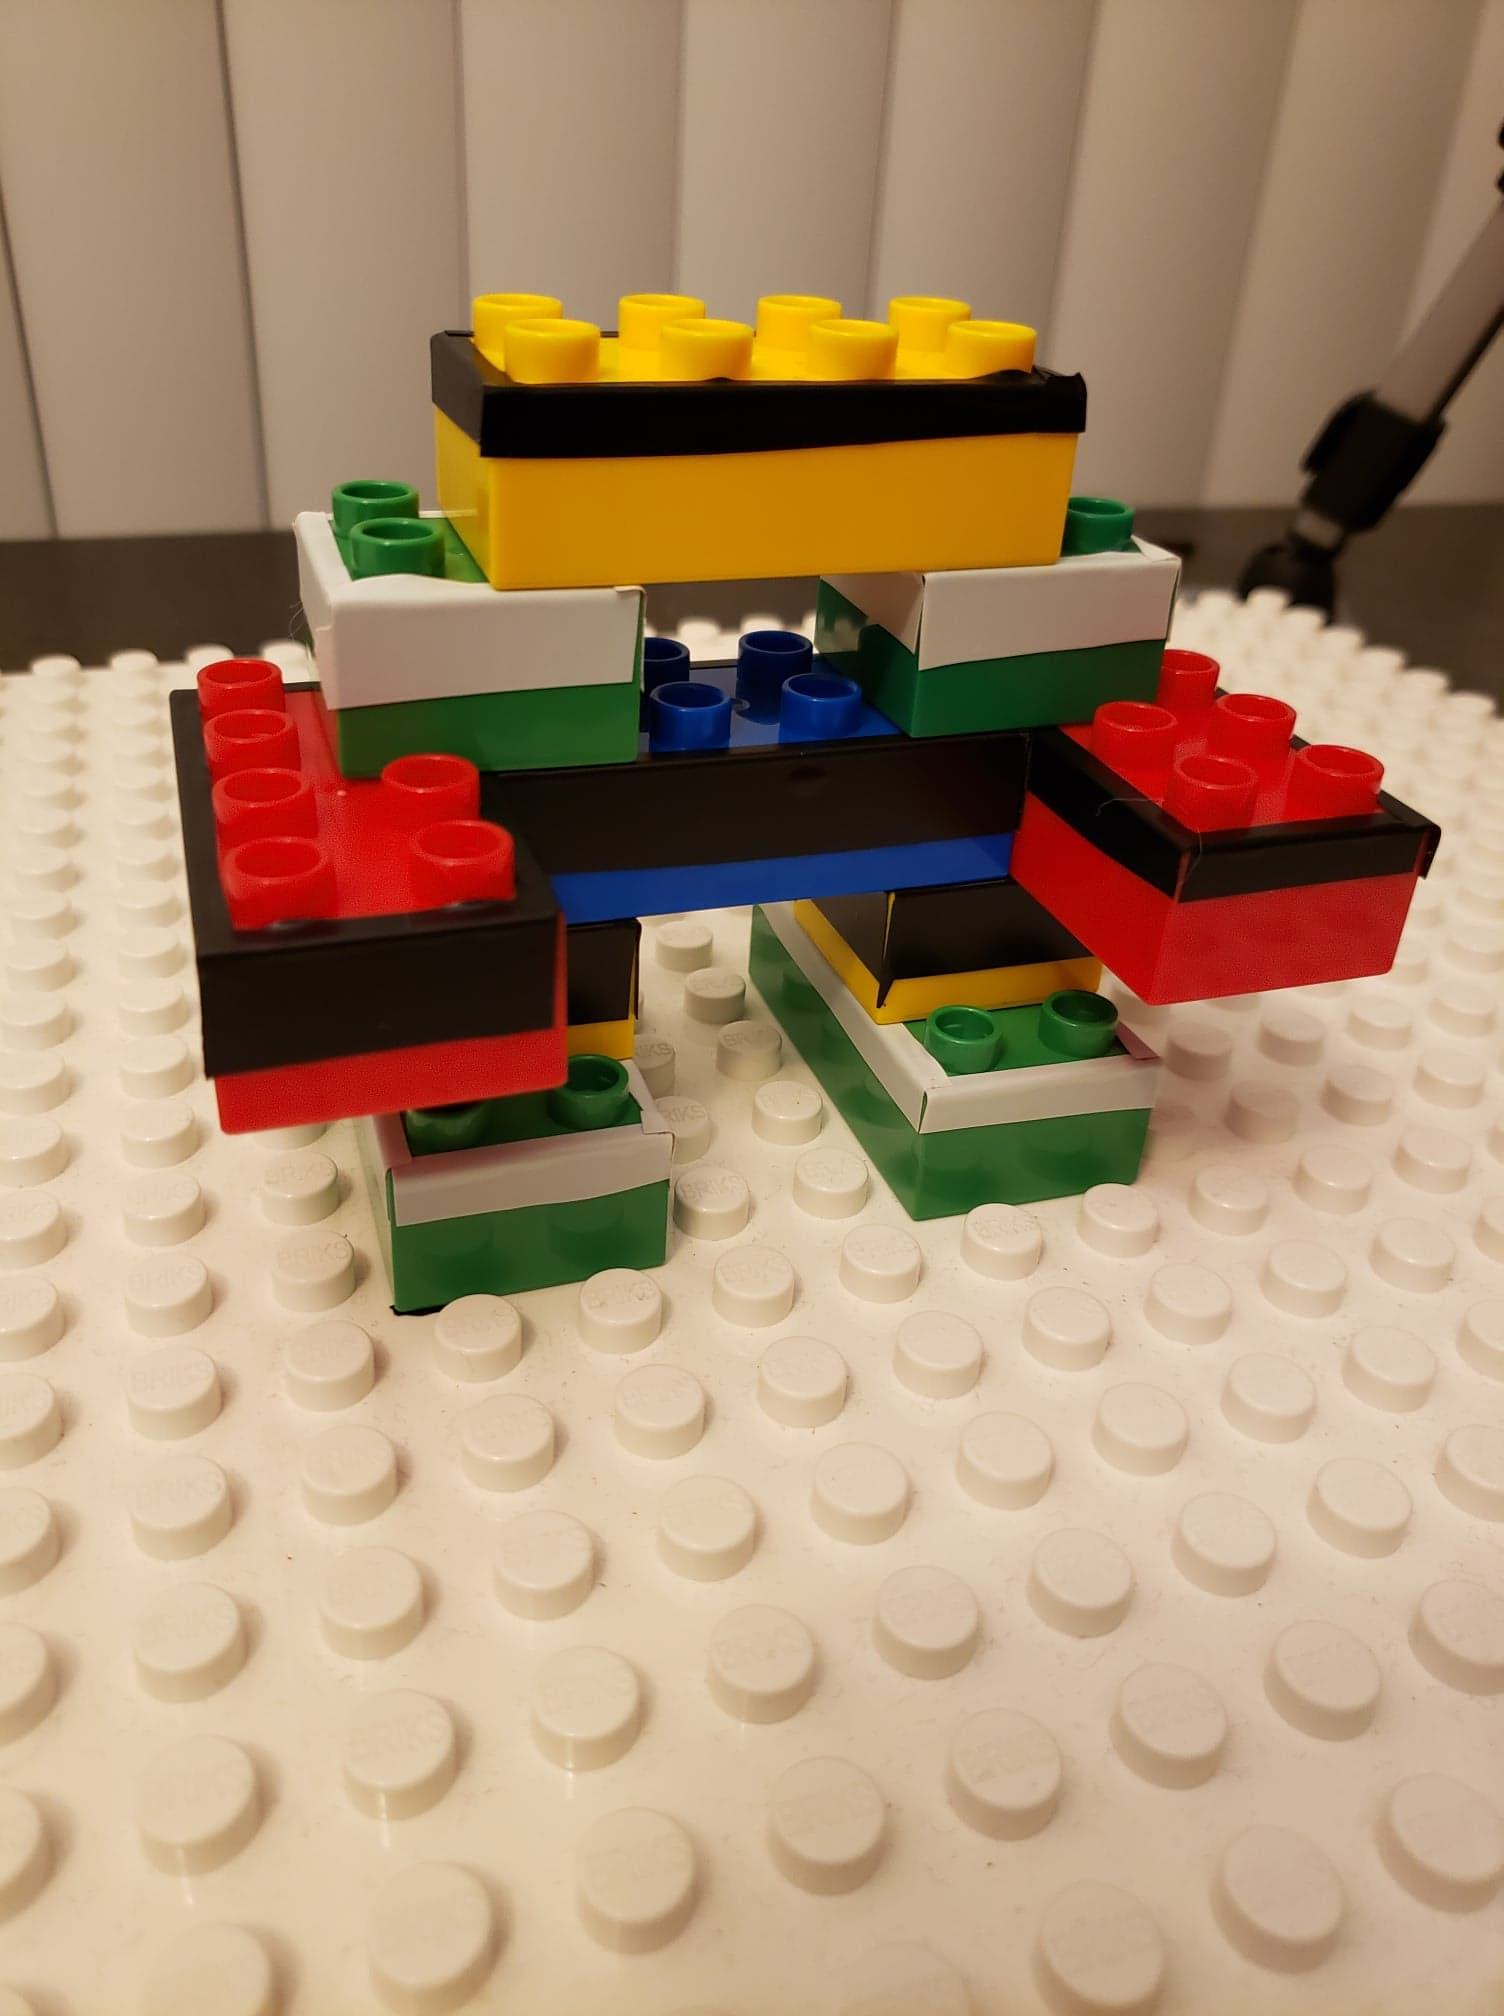
\includegraphics[width=0.8\linewidth,trim={0 25cm 0 5cm},clip]{figures/t1.jpg}
       
       \caption[{}]{\label{fig:fig_3-6a}}
    \end{subfigure}
    \begin{subfigure}{0.5\textwidth}
       \centering
    %   \includegraphics[width=\textwidth,height=\textheight,keepaspectratio]{fig_3-3}
       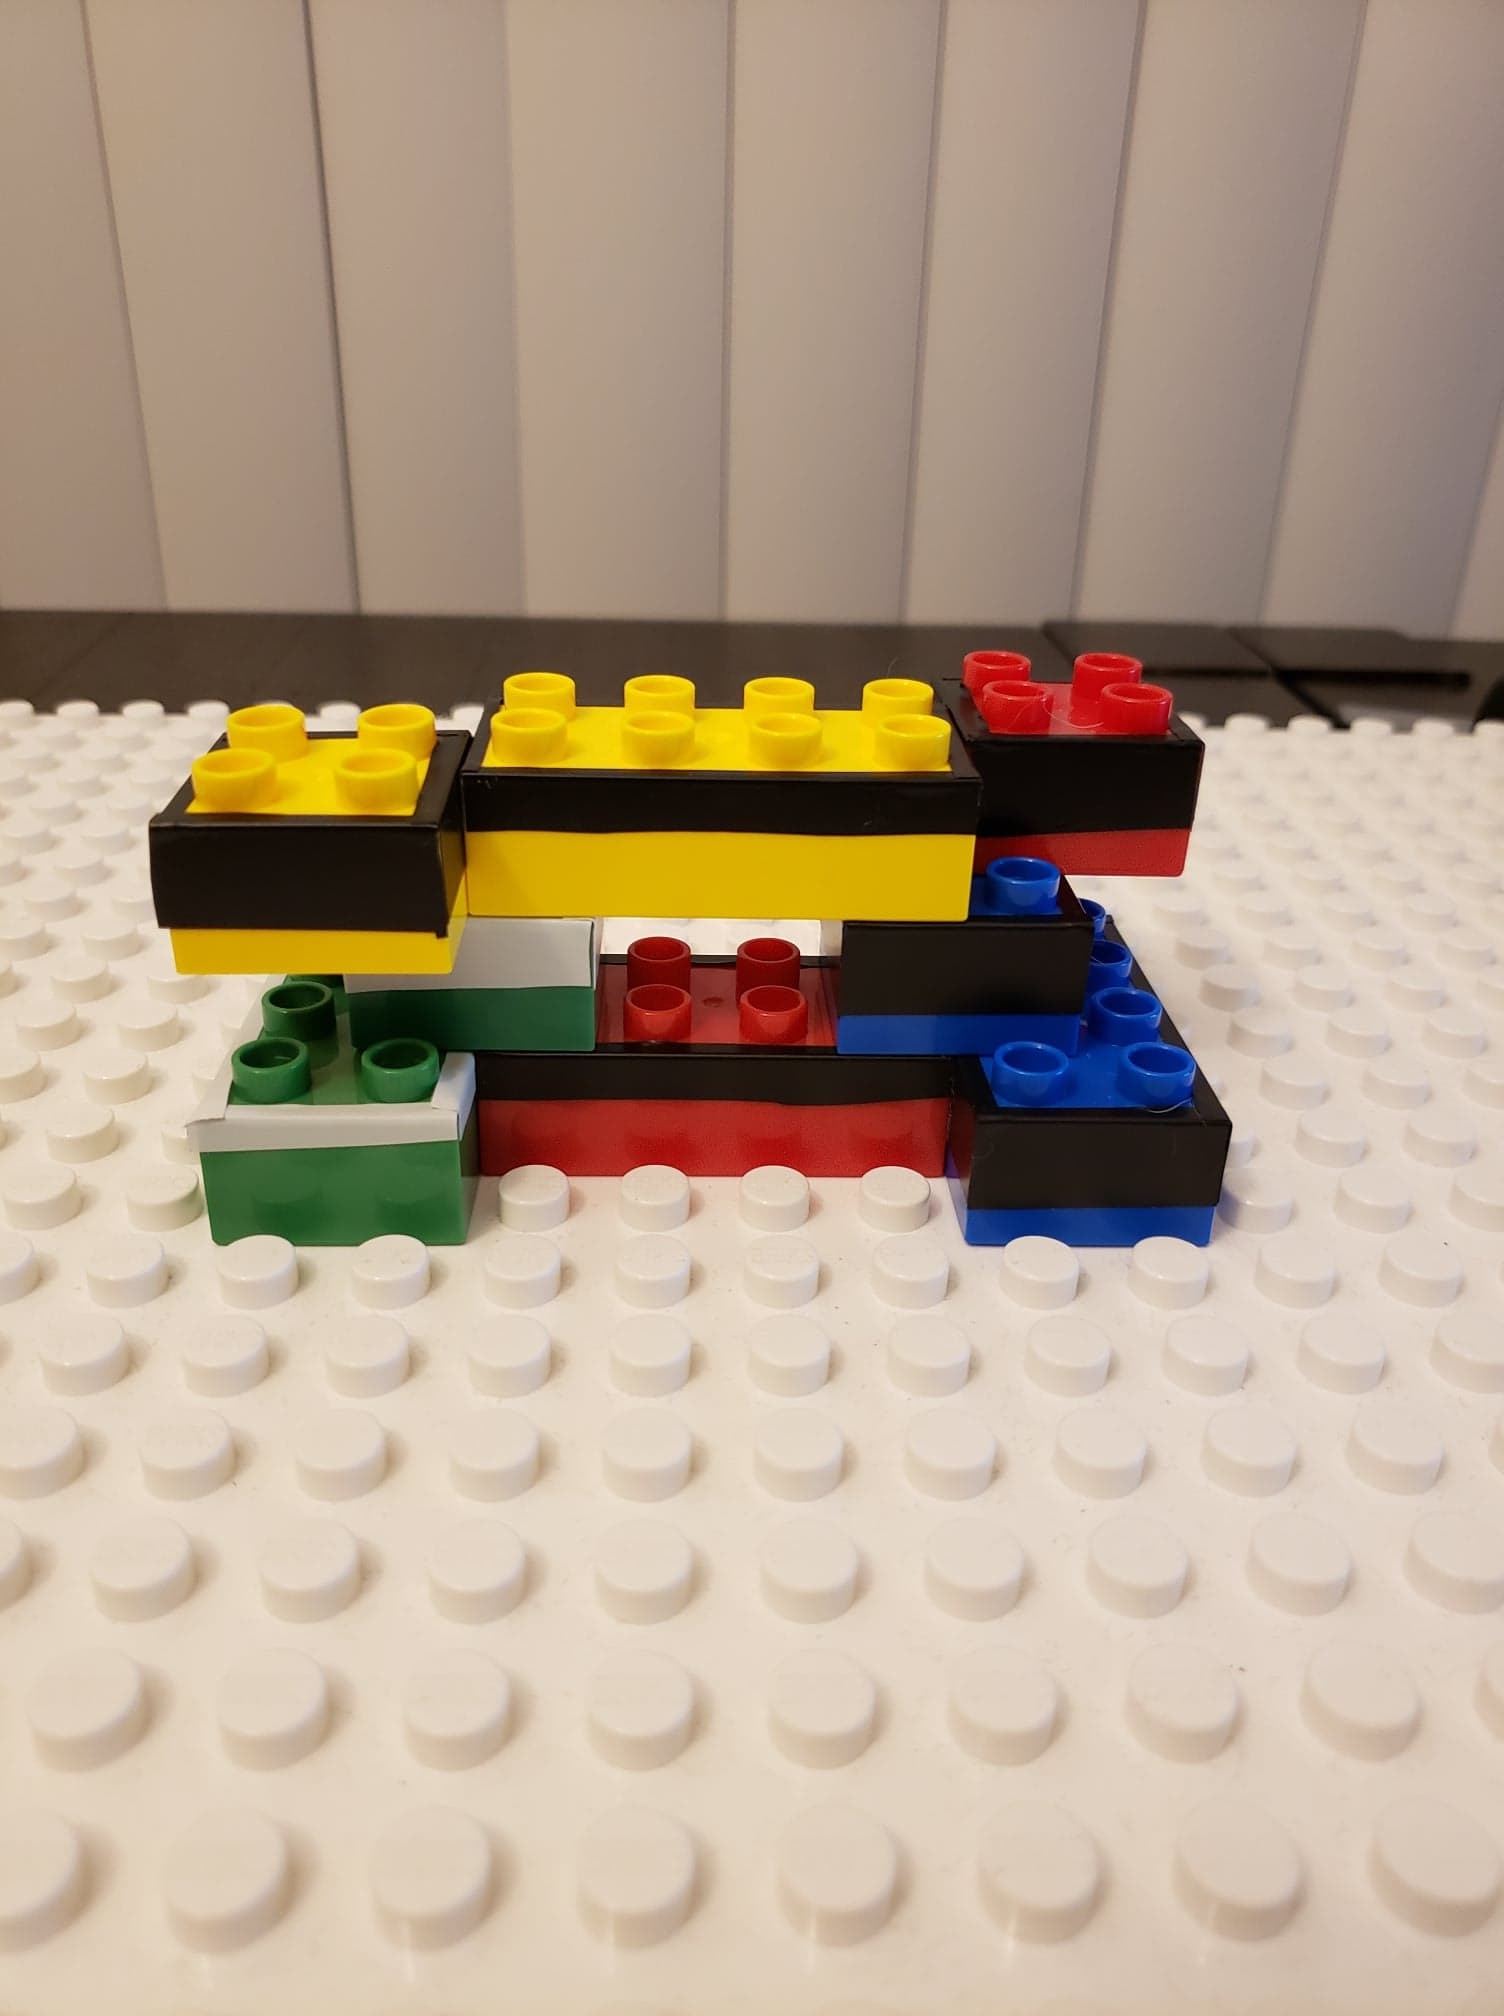
\includegraphics[width=0.8\linewidth,trim={0 20cm 0 10cm},clip]{figures/t2.jpg}
       
       \caption[{}]{\label{fig:fig_3-6b}}
    \end{subfigure}
    \begin{subfigure}{0.5\textwidth}
       \centering
    %   \includegraphics[width=\textwidth,height=\textheight,keepaspectratio]{fig_3-3}
       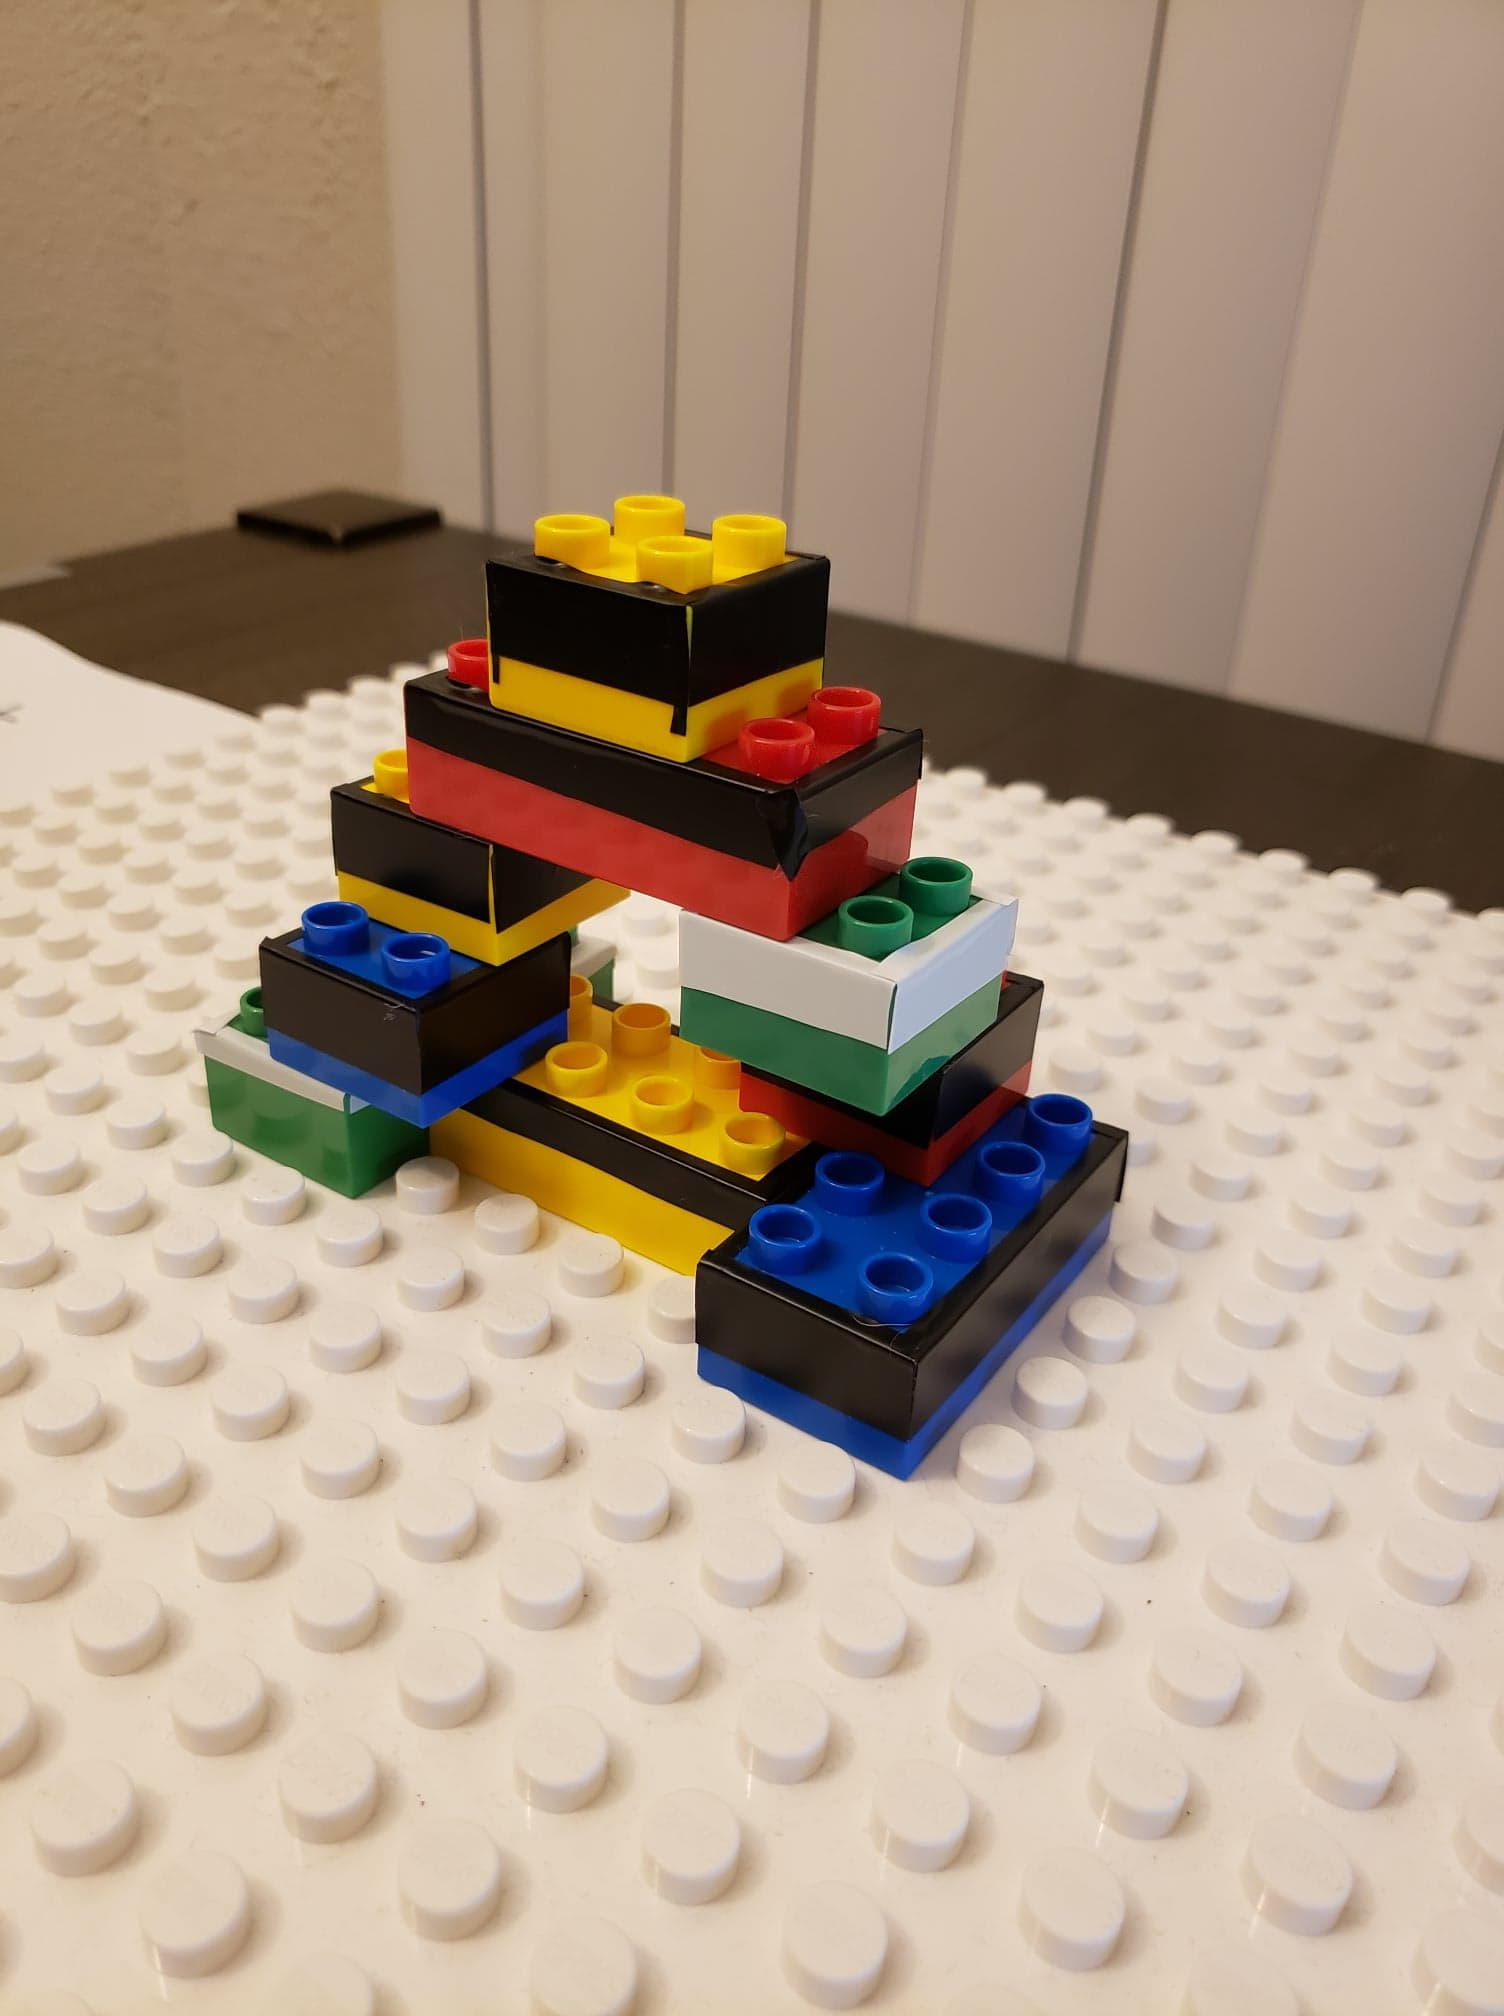
\includegraphics[width=0.8\linewidth,trim={0 15cm 0 15cm},clip]{figures/t3.jpg}
       
       \caption[{}]{\label{fig:fig_3-6c}}
    \end{subfigure}
    \begin{subfigure}{0.5\textwidth}
       \centering
    %   \includegraphics[width=\textwidth,height=\textheight,keepaspectratio]{fig_3-3}
       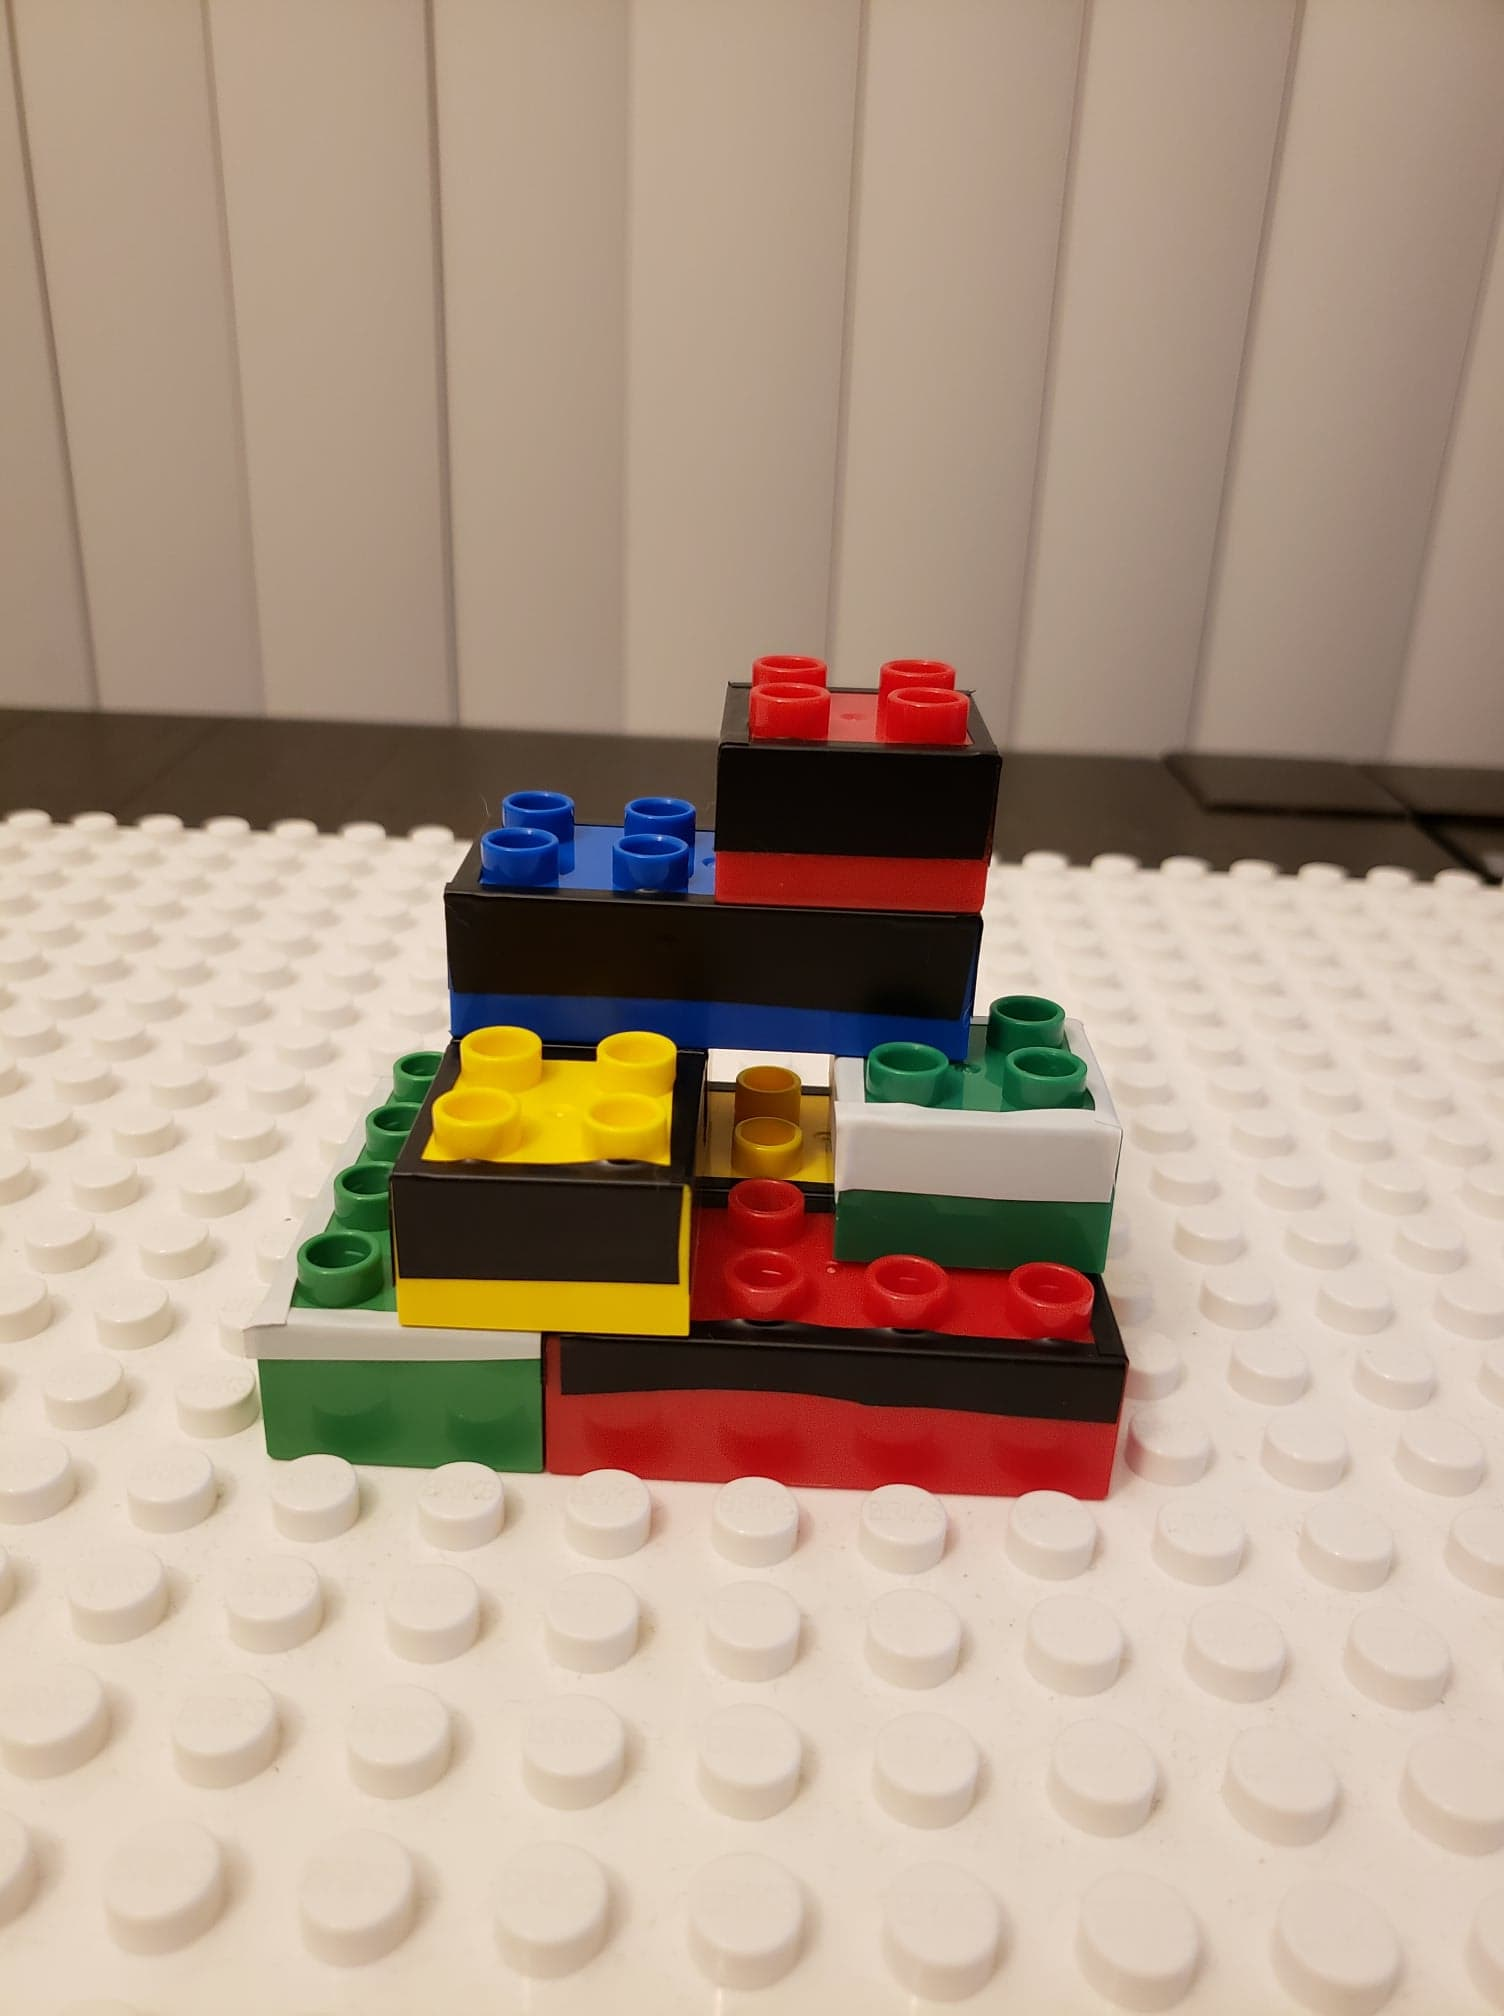
\includegraphics[width=0.8\linewidth,trim={0 15cm 0 15cm},clip]{figures/t4.jpg}
       
       \caption[{}]{\label{fig:fig_3-6d}}
    \end{subfigure}
    \begin{subfigure}{0.5\textwidth}
       \centering
    %   \includegraphics[width=\textwidth,height=\textheight,keepaspectratio]{fig_3-3}
       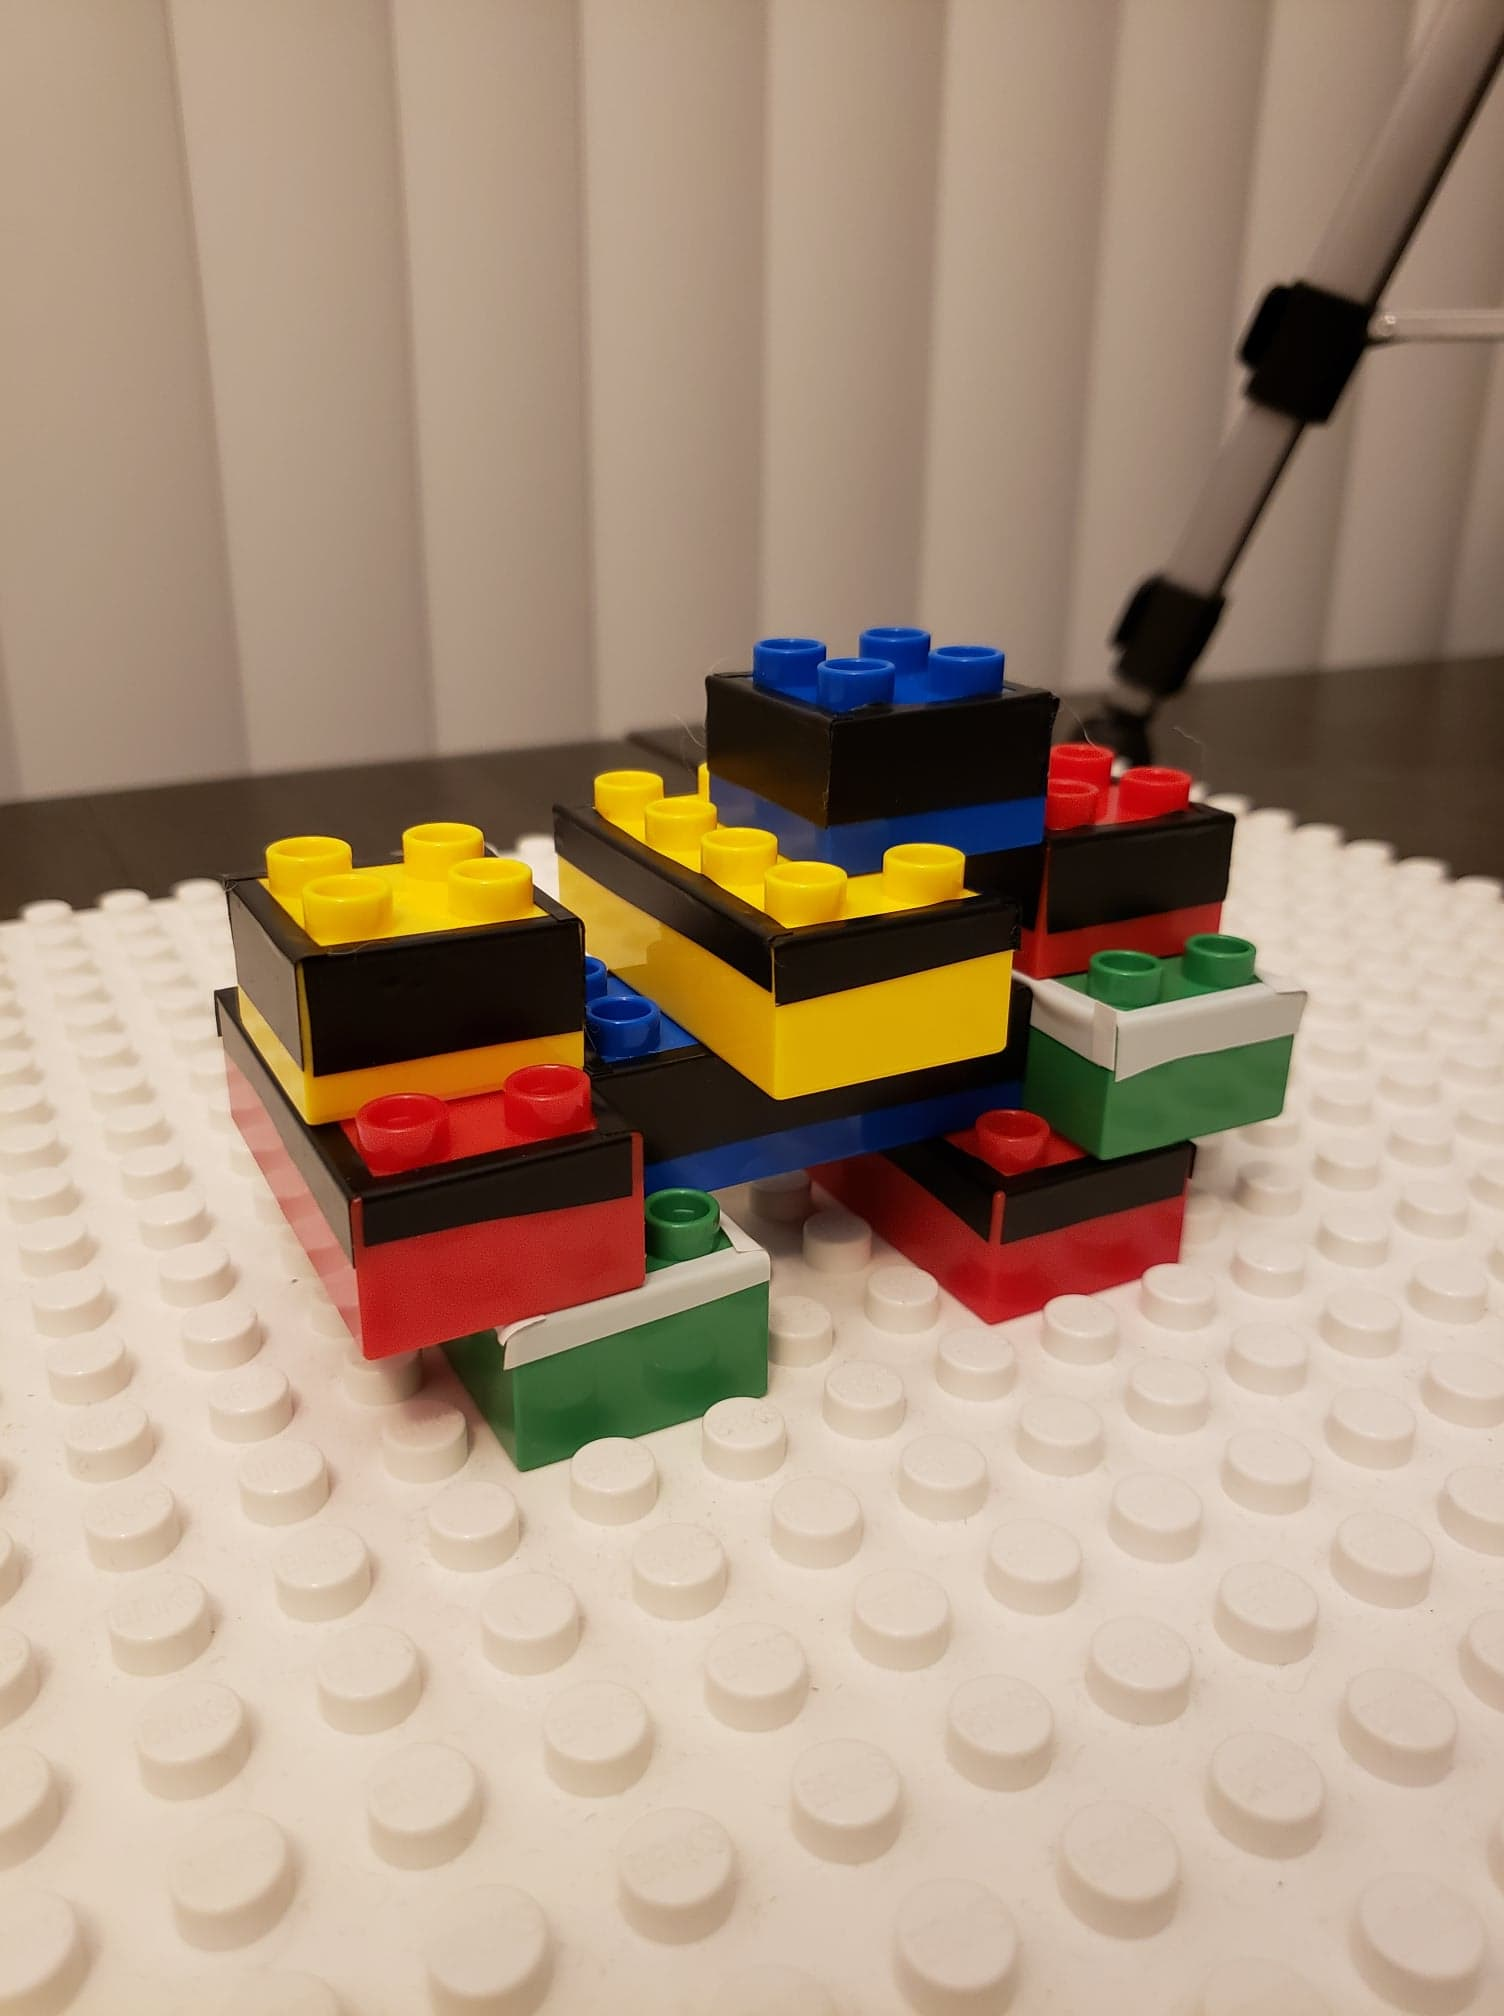
\includegraphics[width=0.8\linewidth,trim={0 10cm 0 20cm},clip]{figures/t6.jpg}
      
       \caption[{}]{ \label{fig:fig_3-6e}}
    \end{subfigure}
    \begin{subfigure}{0.5\textwidth}
       \centering
    %   \includegraphics[width=\textwidth,height=\textheight,keepaspectratio]{fig_3-3}
       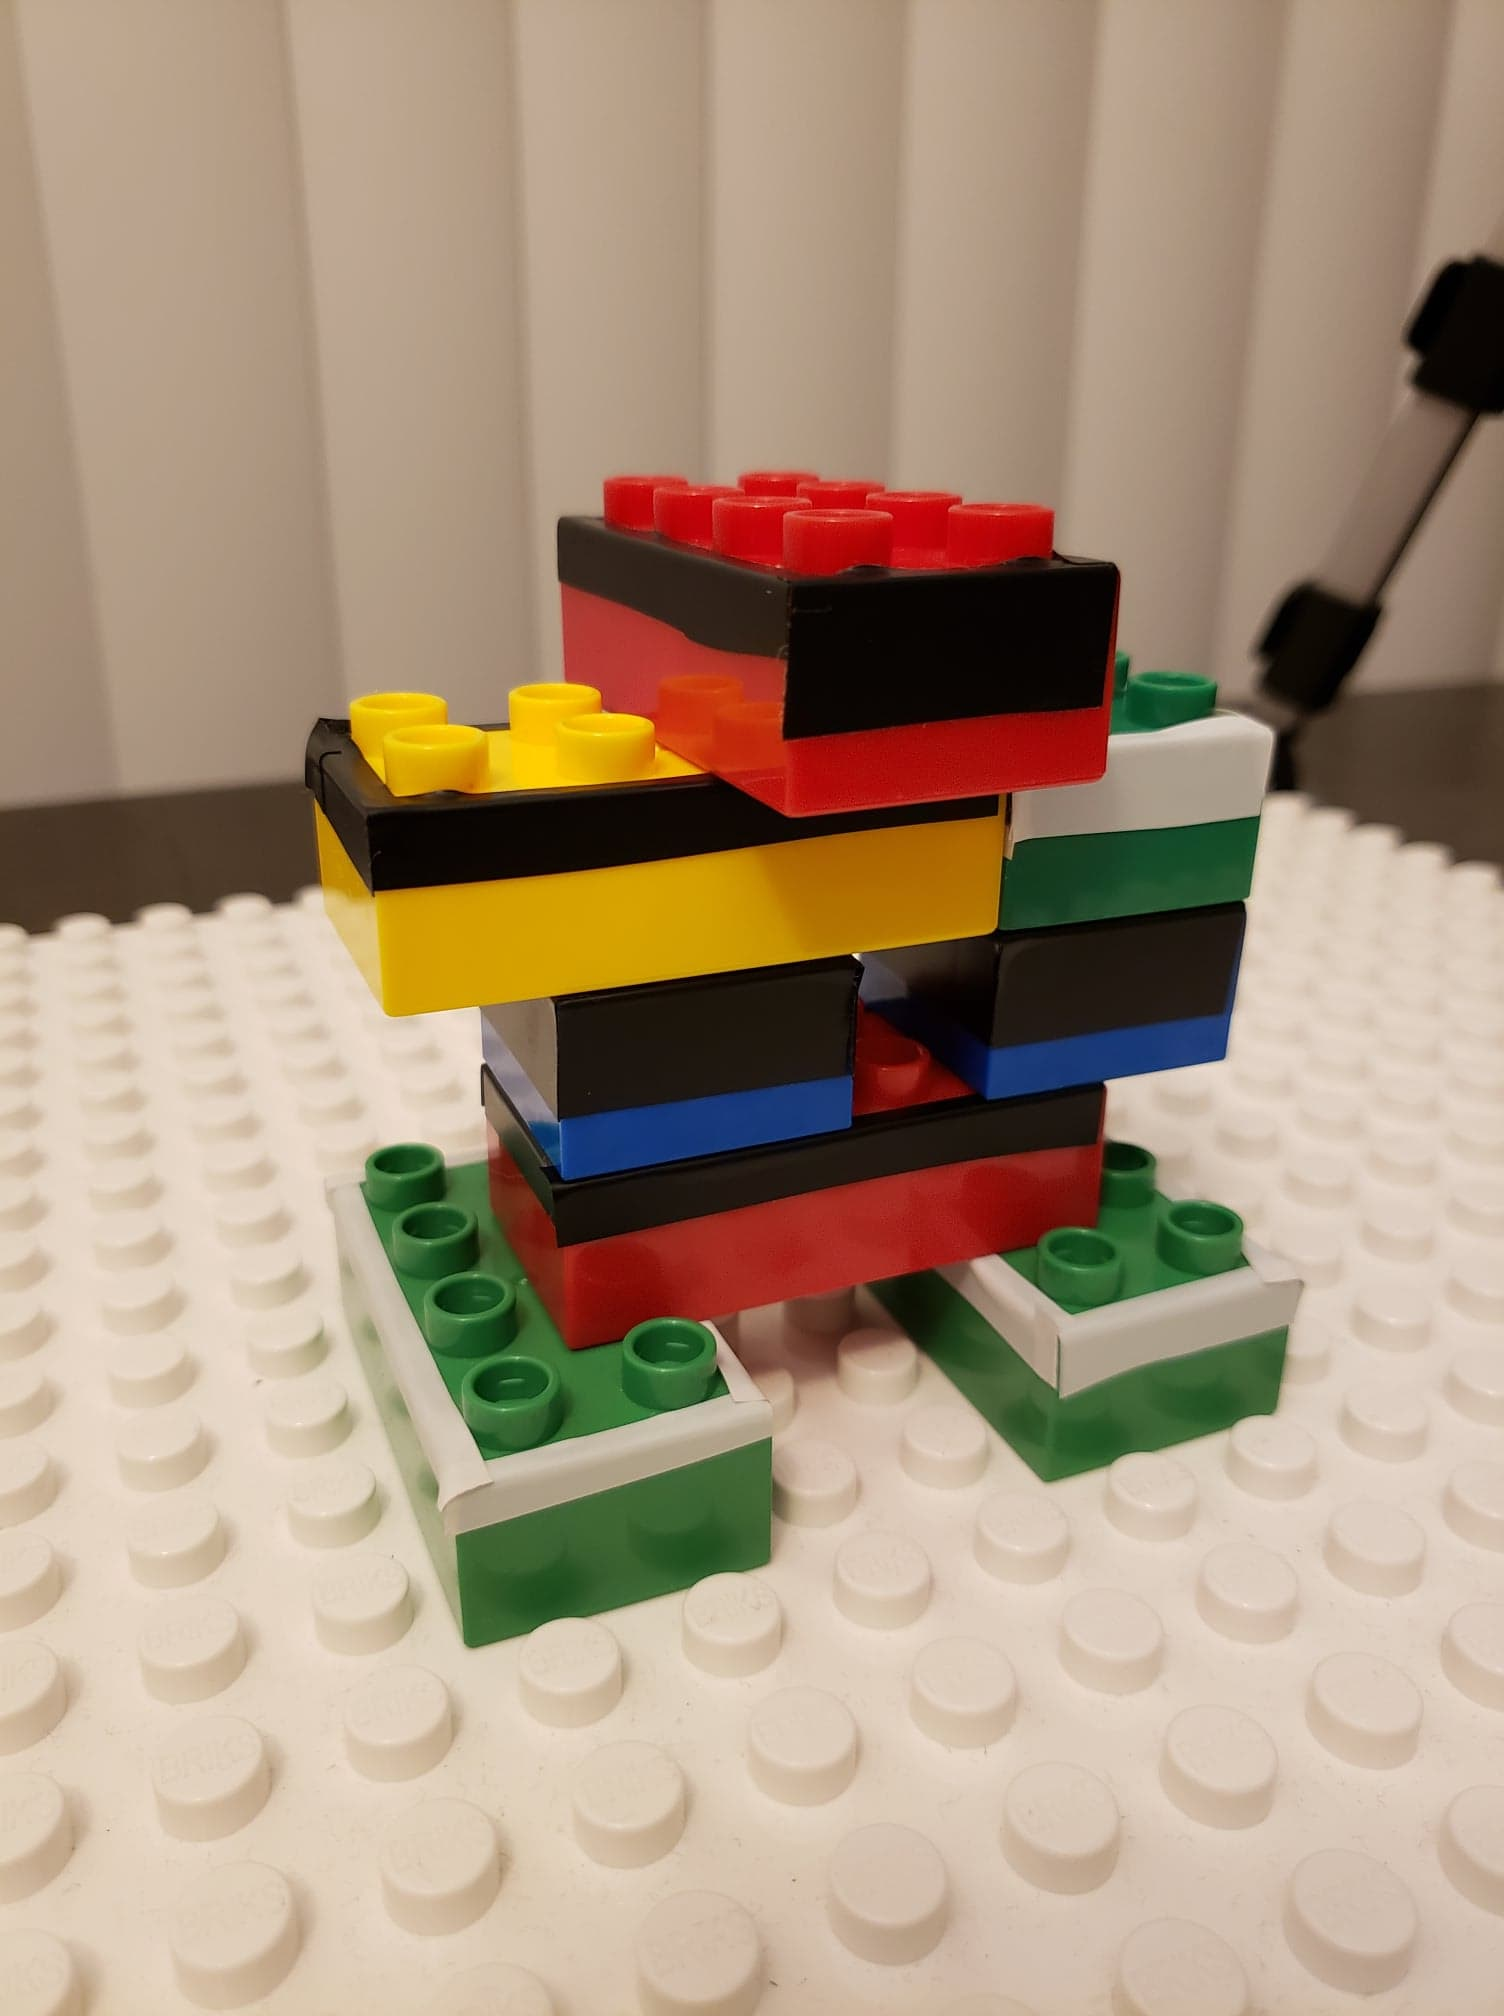
\includegraphics[width=0.8\linewidth,trim={0 15cm 0 15cm},clip]{figures/t7.jpg}
       
       \caption[{}]{\label{fig:fig_3-6f}}
    \end{subfigure}
    \begin{subfigure}{0.5\textwidth}
       \centering
    %   \includegraphics[width=\textwidth,height=\textheight,keepaspectratio]{fig_3-3}
       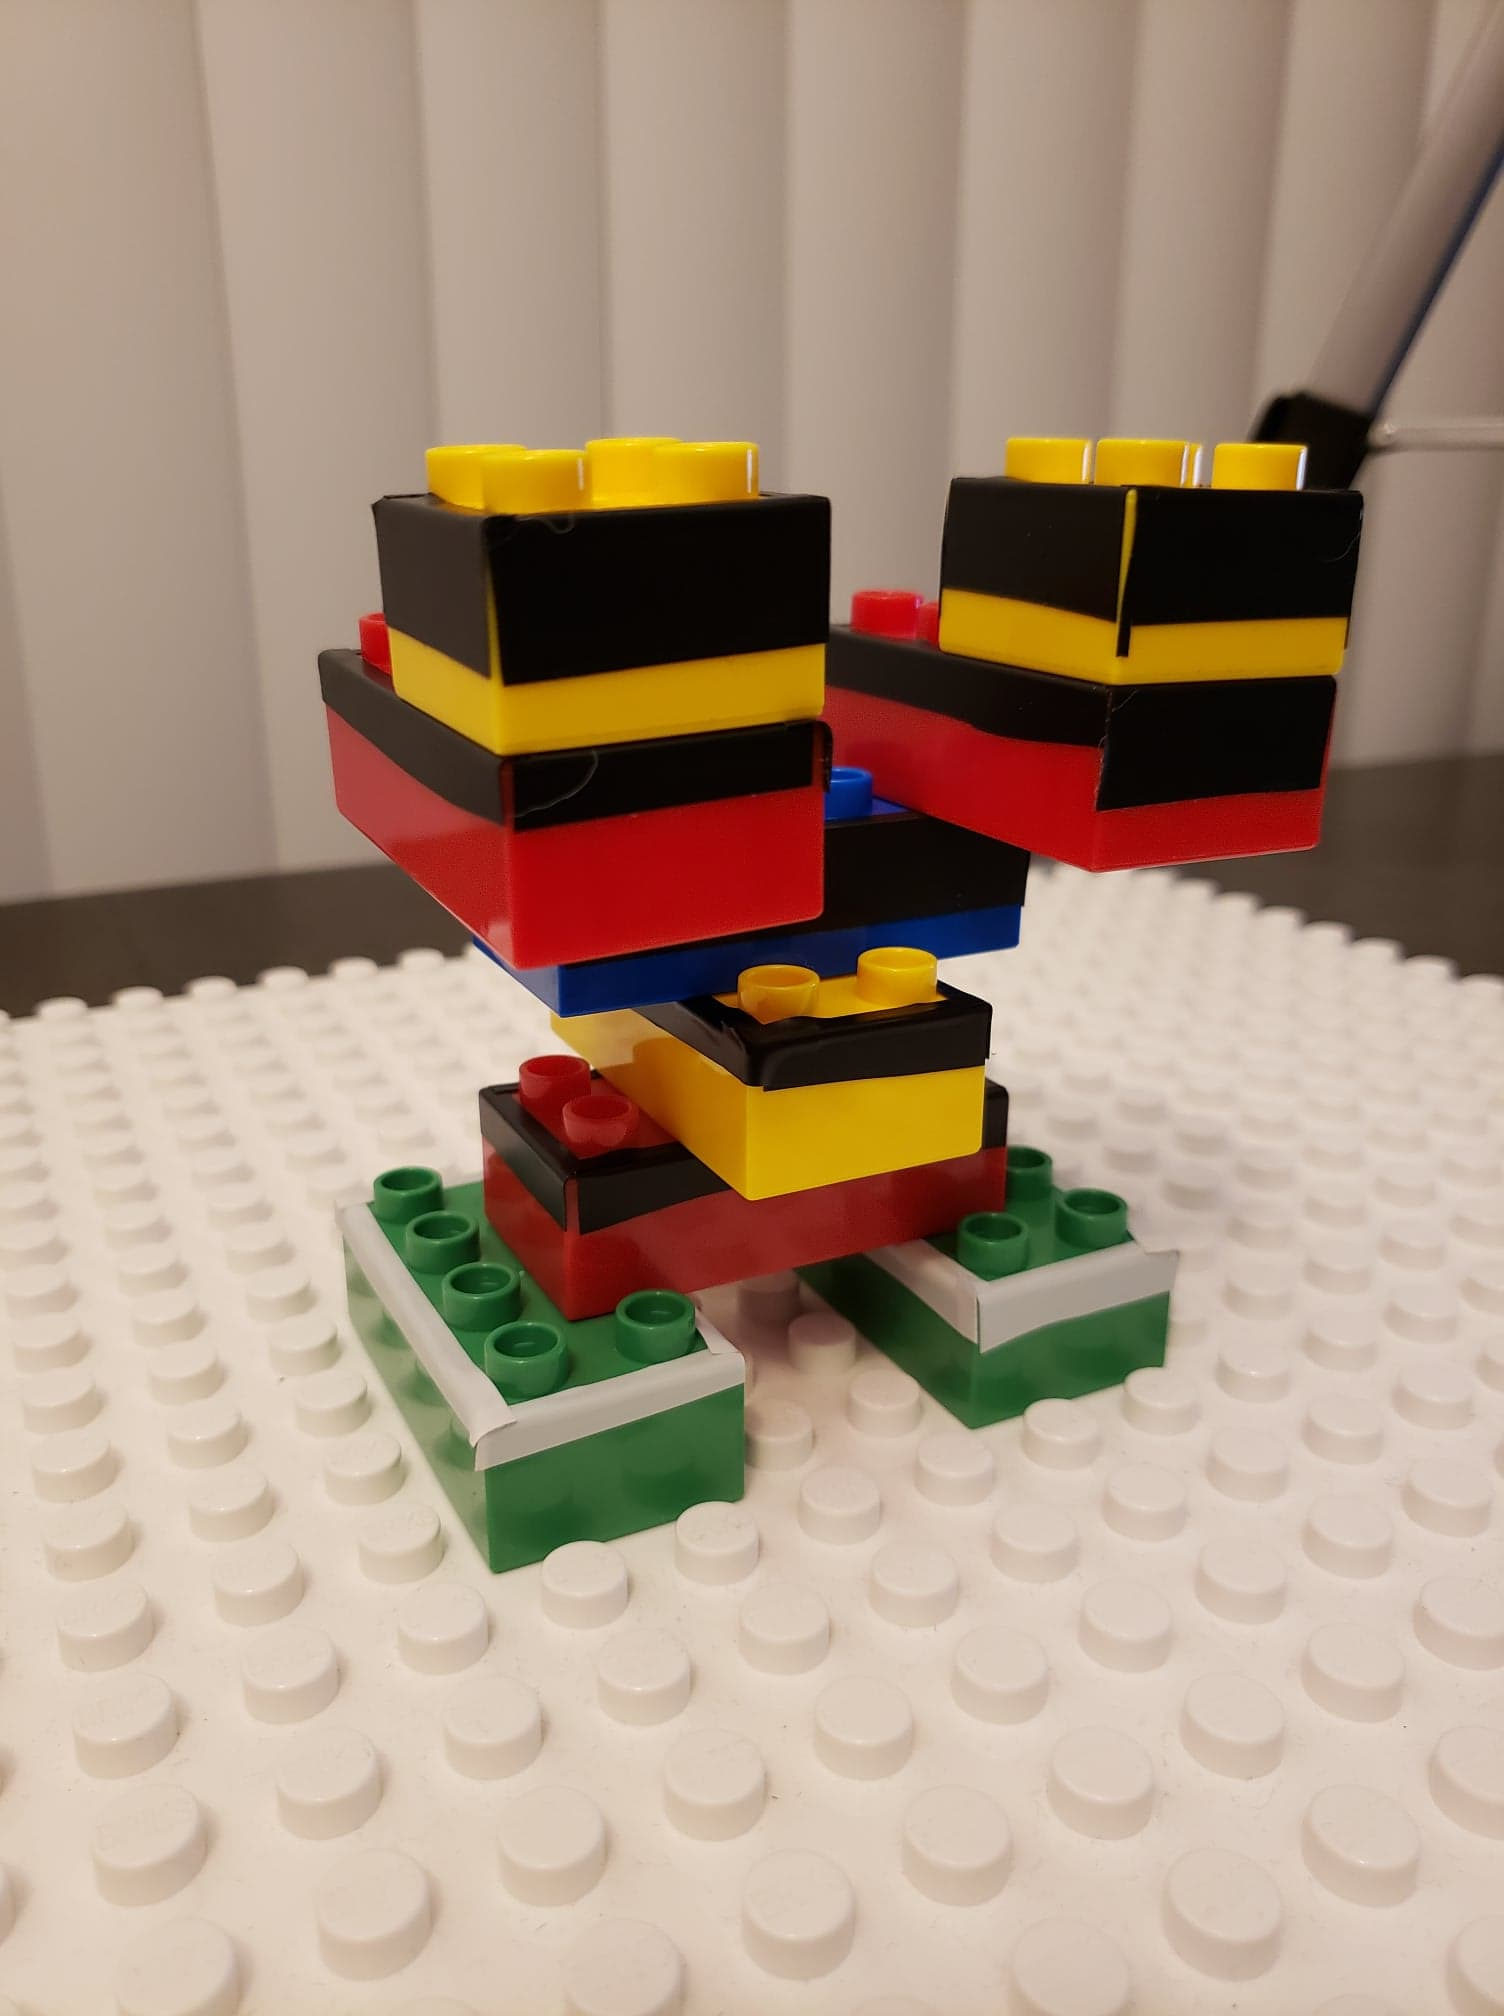
\includegraphics[width=0.8\linewidth,trim={0 15cm 0 15cm},clip]{figures/t5.jpg}
      
       \caption[{}]{ \label{fig:fig_3-6g}}
    \end{subfigure}
    \caption[{Simple 3D structures}]{Simple 3D structures successfully completed in both learning and teaching modes.}
   \label{fig:fig_3-6}
\end{figure}
% Figure 3-7
\begin{figure}[H]
    \begin{subfigure}{0.5\textwidth}
       \centering
    %   \includegraphics[width=\textwidth,height=\textheight,keepaspectratio]{fig_3-3}
       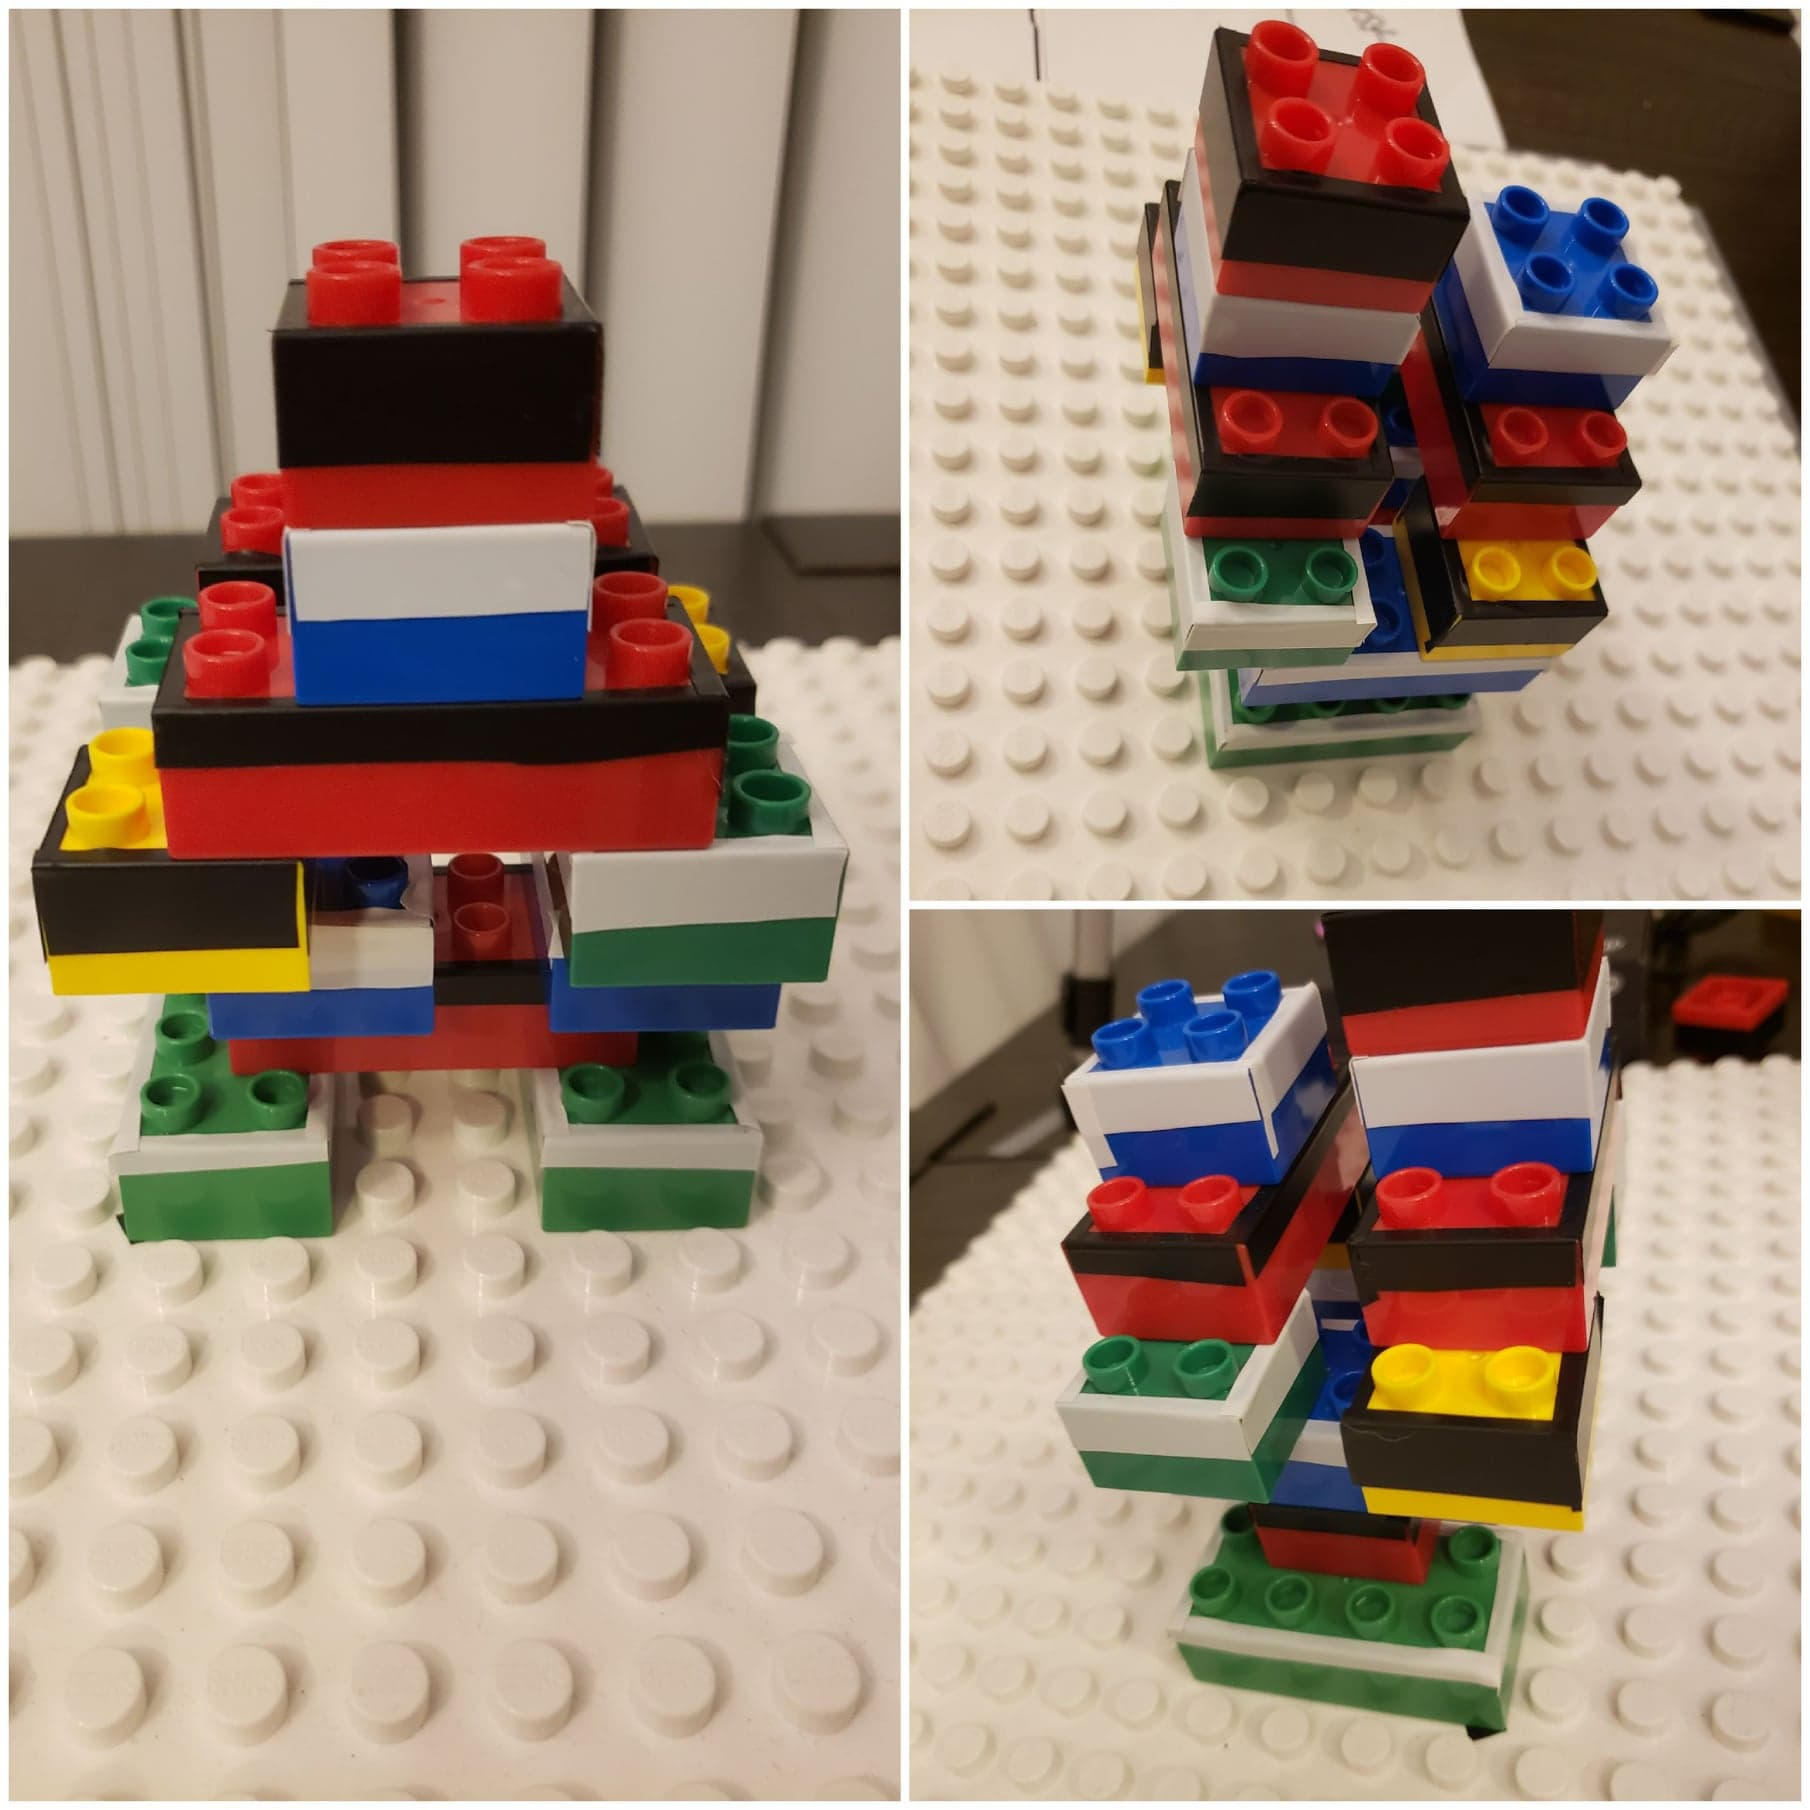
\includegraphics[width=0.8\linewidth]{figures/e3.jpg}
       
       \caption[{}]{\label{fig:fig_3-7a}}
    \end{subfigure}
    \begin{subfigure}{0.5\textwidth}
       \centering
    %   \includegraphics[width=\textwidth,height=\textheight,keepaspectratio]{fig_3-3}
       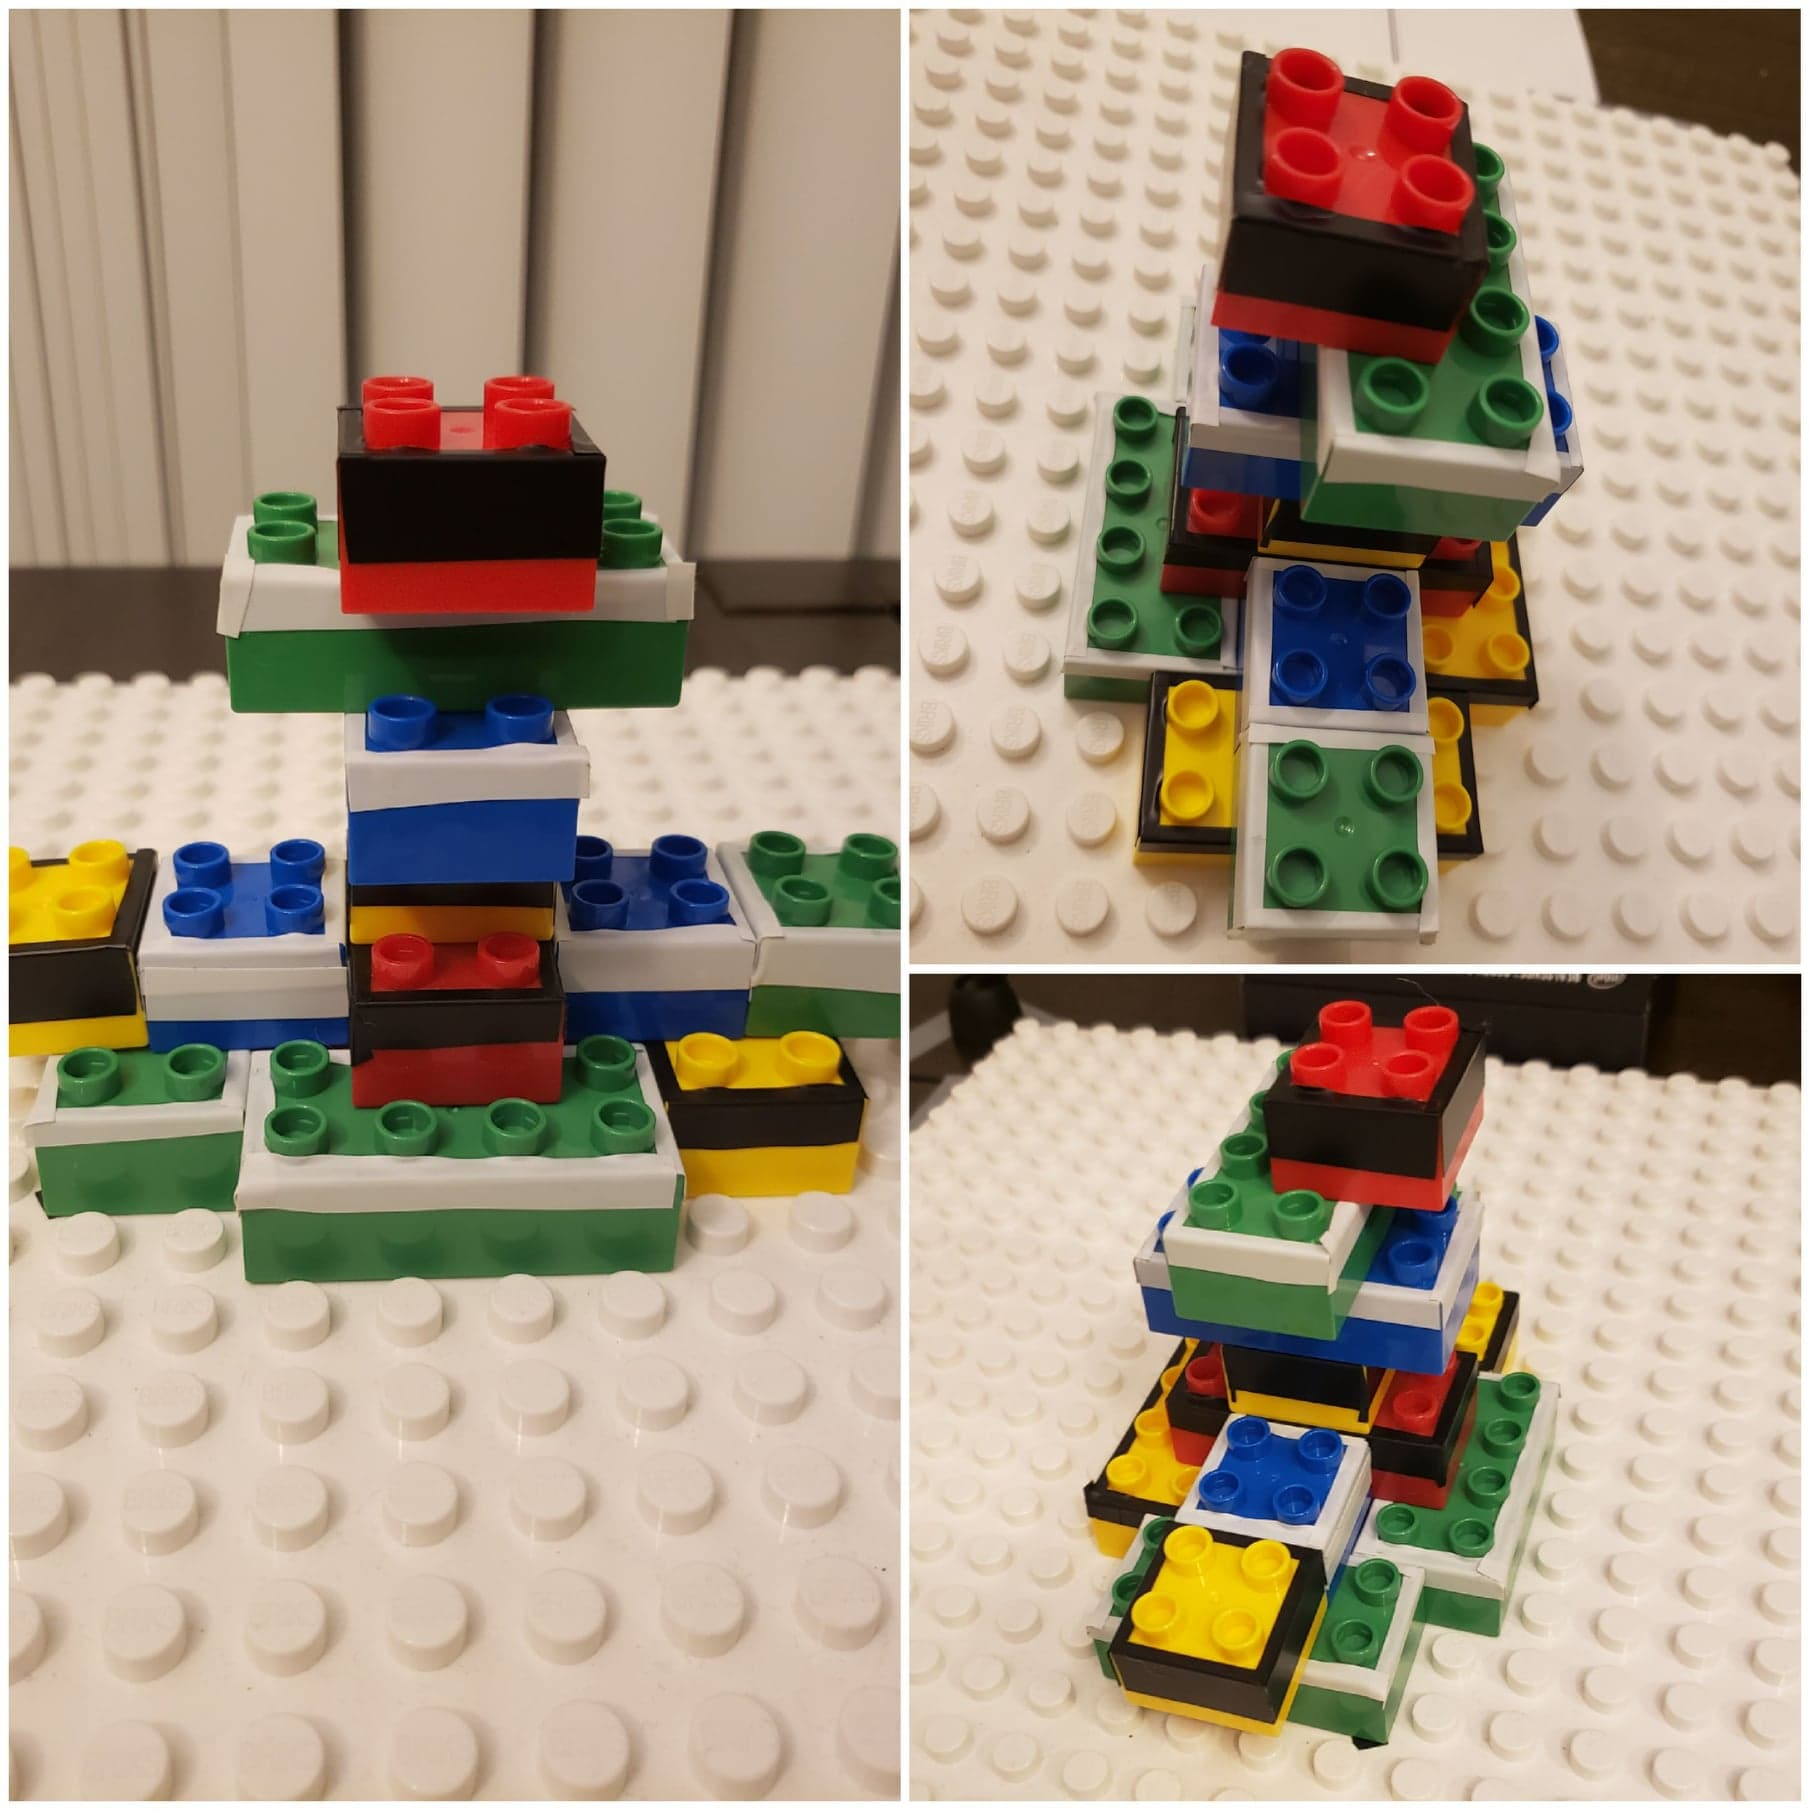
\includegraphics[width=0.8\linewidth]{figures/e4.jpg}
       
       \caption[{}]{\label{fig:fig_3-7b}}
    \end{subfigure}
    \begin{subfigure}{0.5\textwidth}
       \centering
    %   \includegraphics[width=\textwidth,height=\textheight,keepaspectratio]{fig_3-3}
       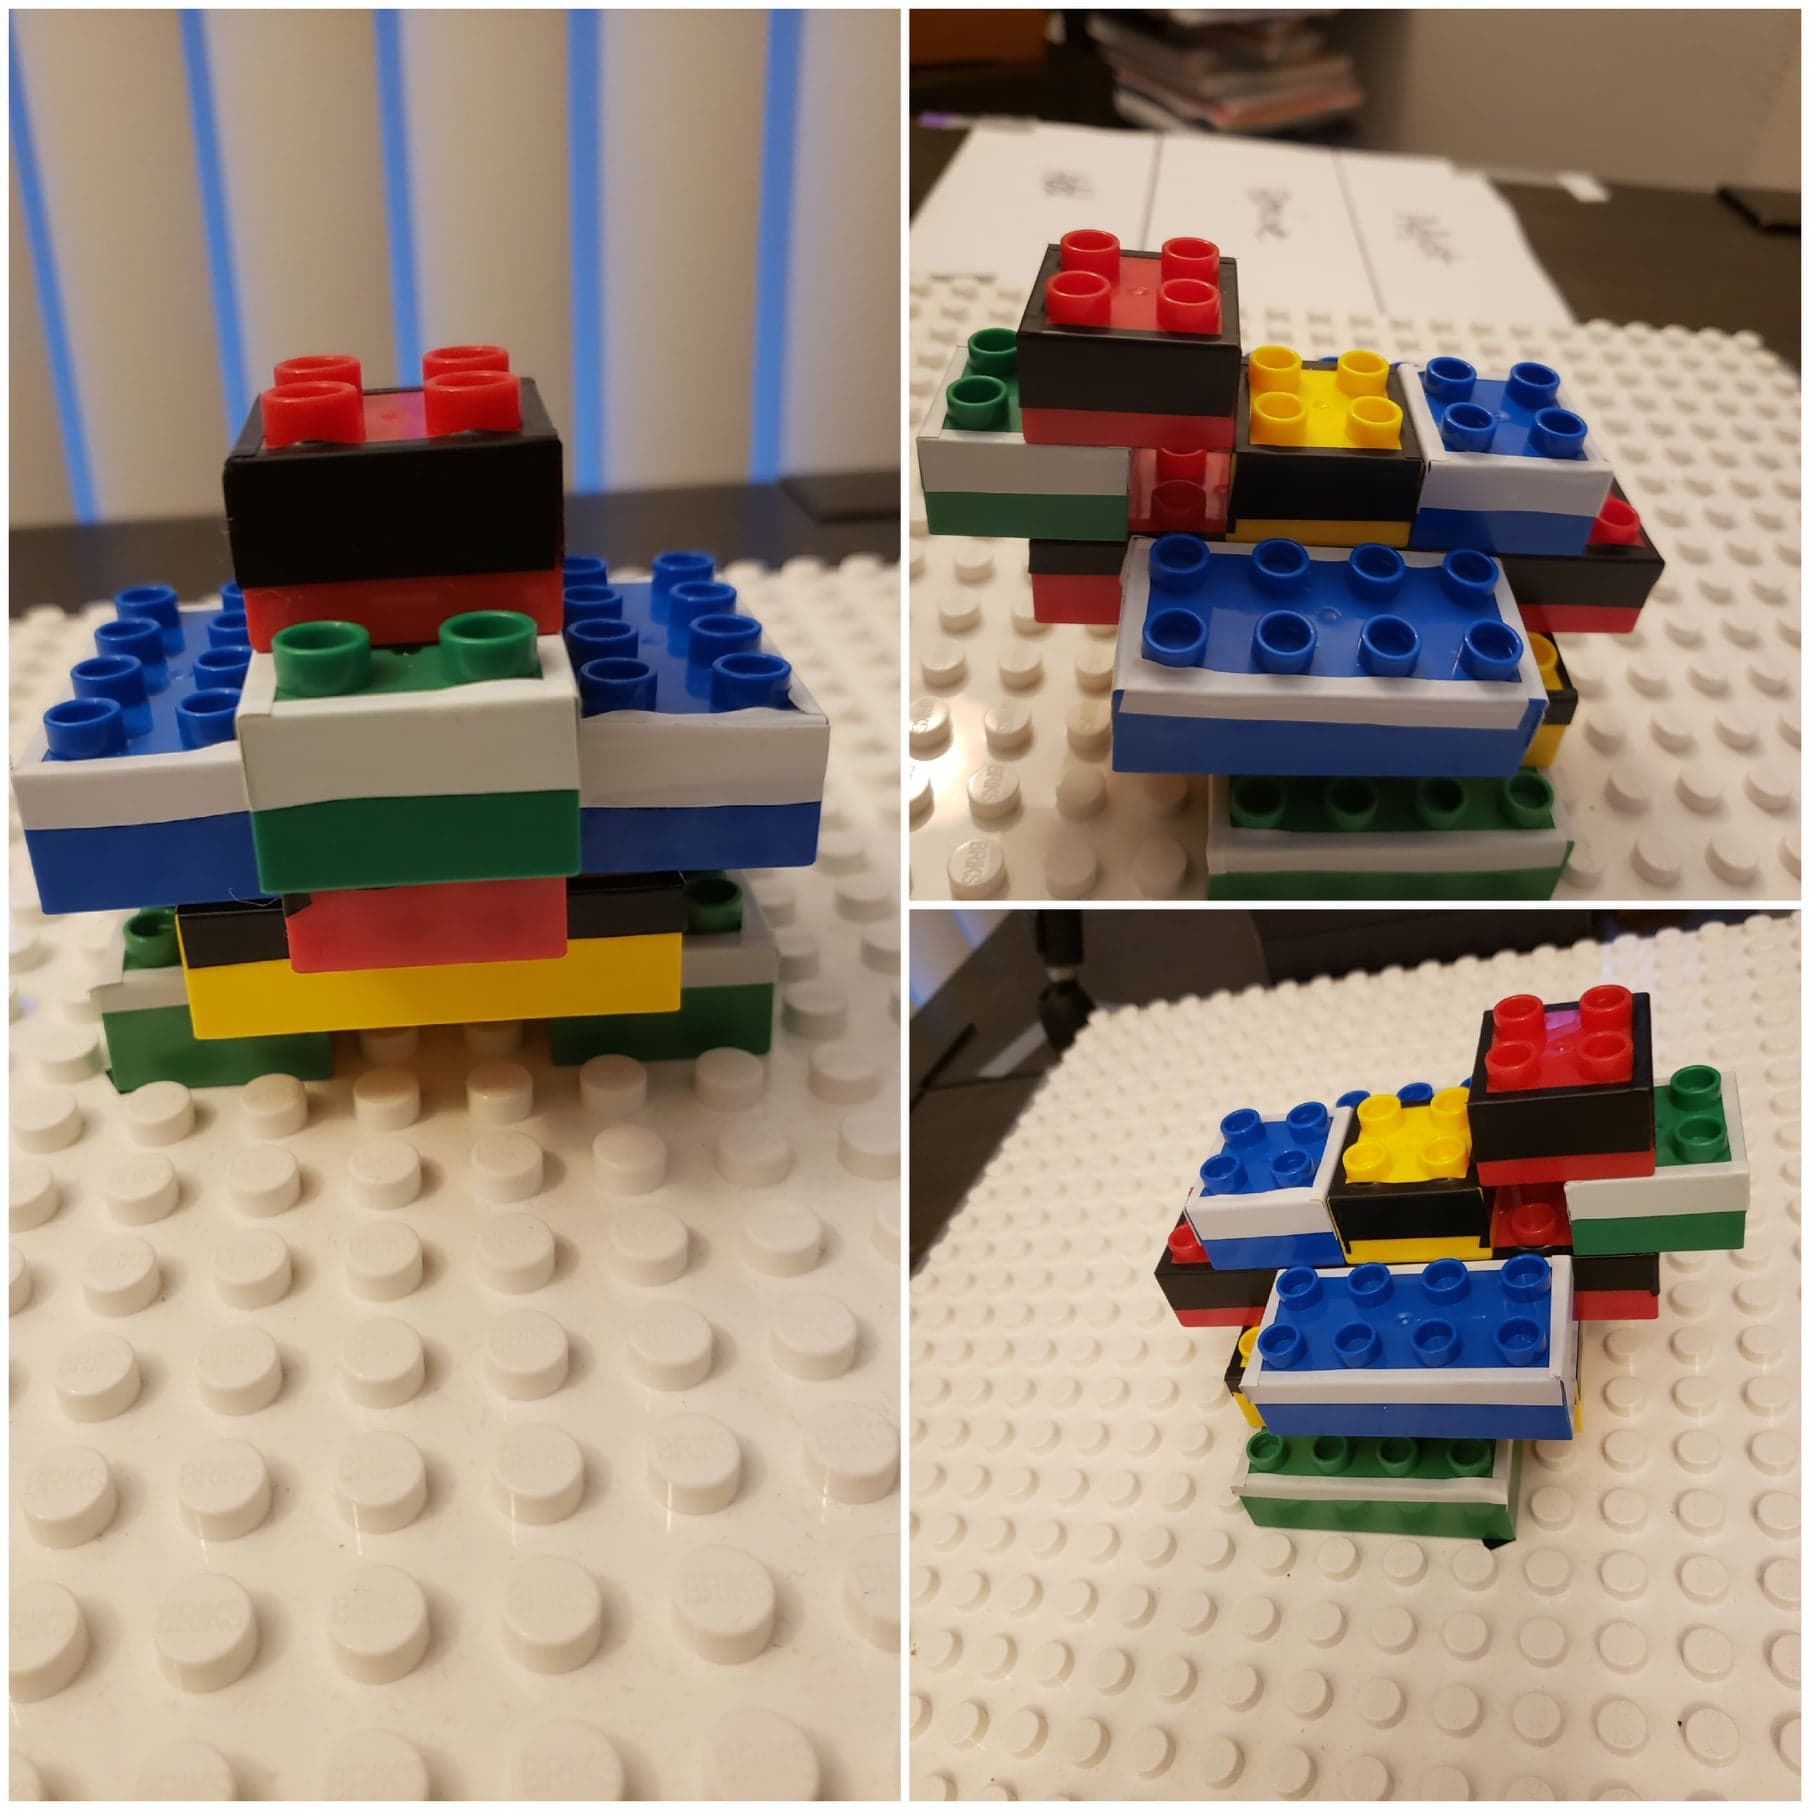
\includegraphics[width=0.8\linewidth]{figures/e5.jpg}
      
       \caption[{}]{ \label{fig:fig_3-7c}}
    \end{subfigure}
    \begin{subfigure}{0.5\textwidth}
       \centering
    %   \includegraphics[width=\textwidth,height=\textheight,keepaspectratio]{fig_3-3}
       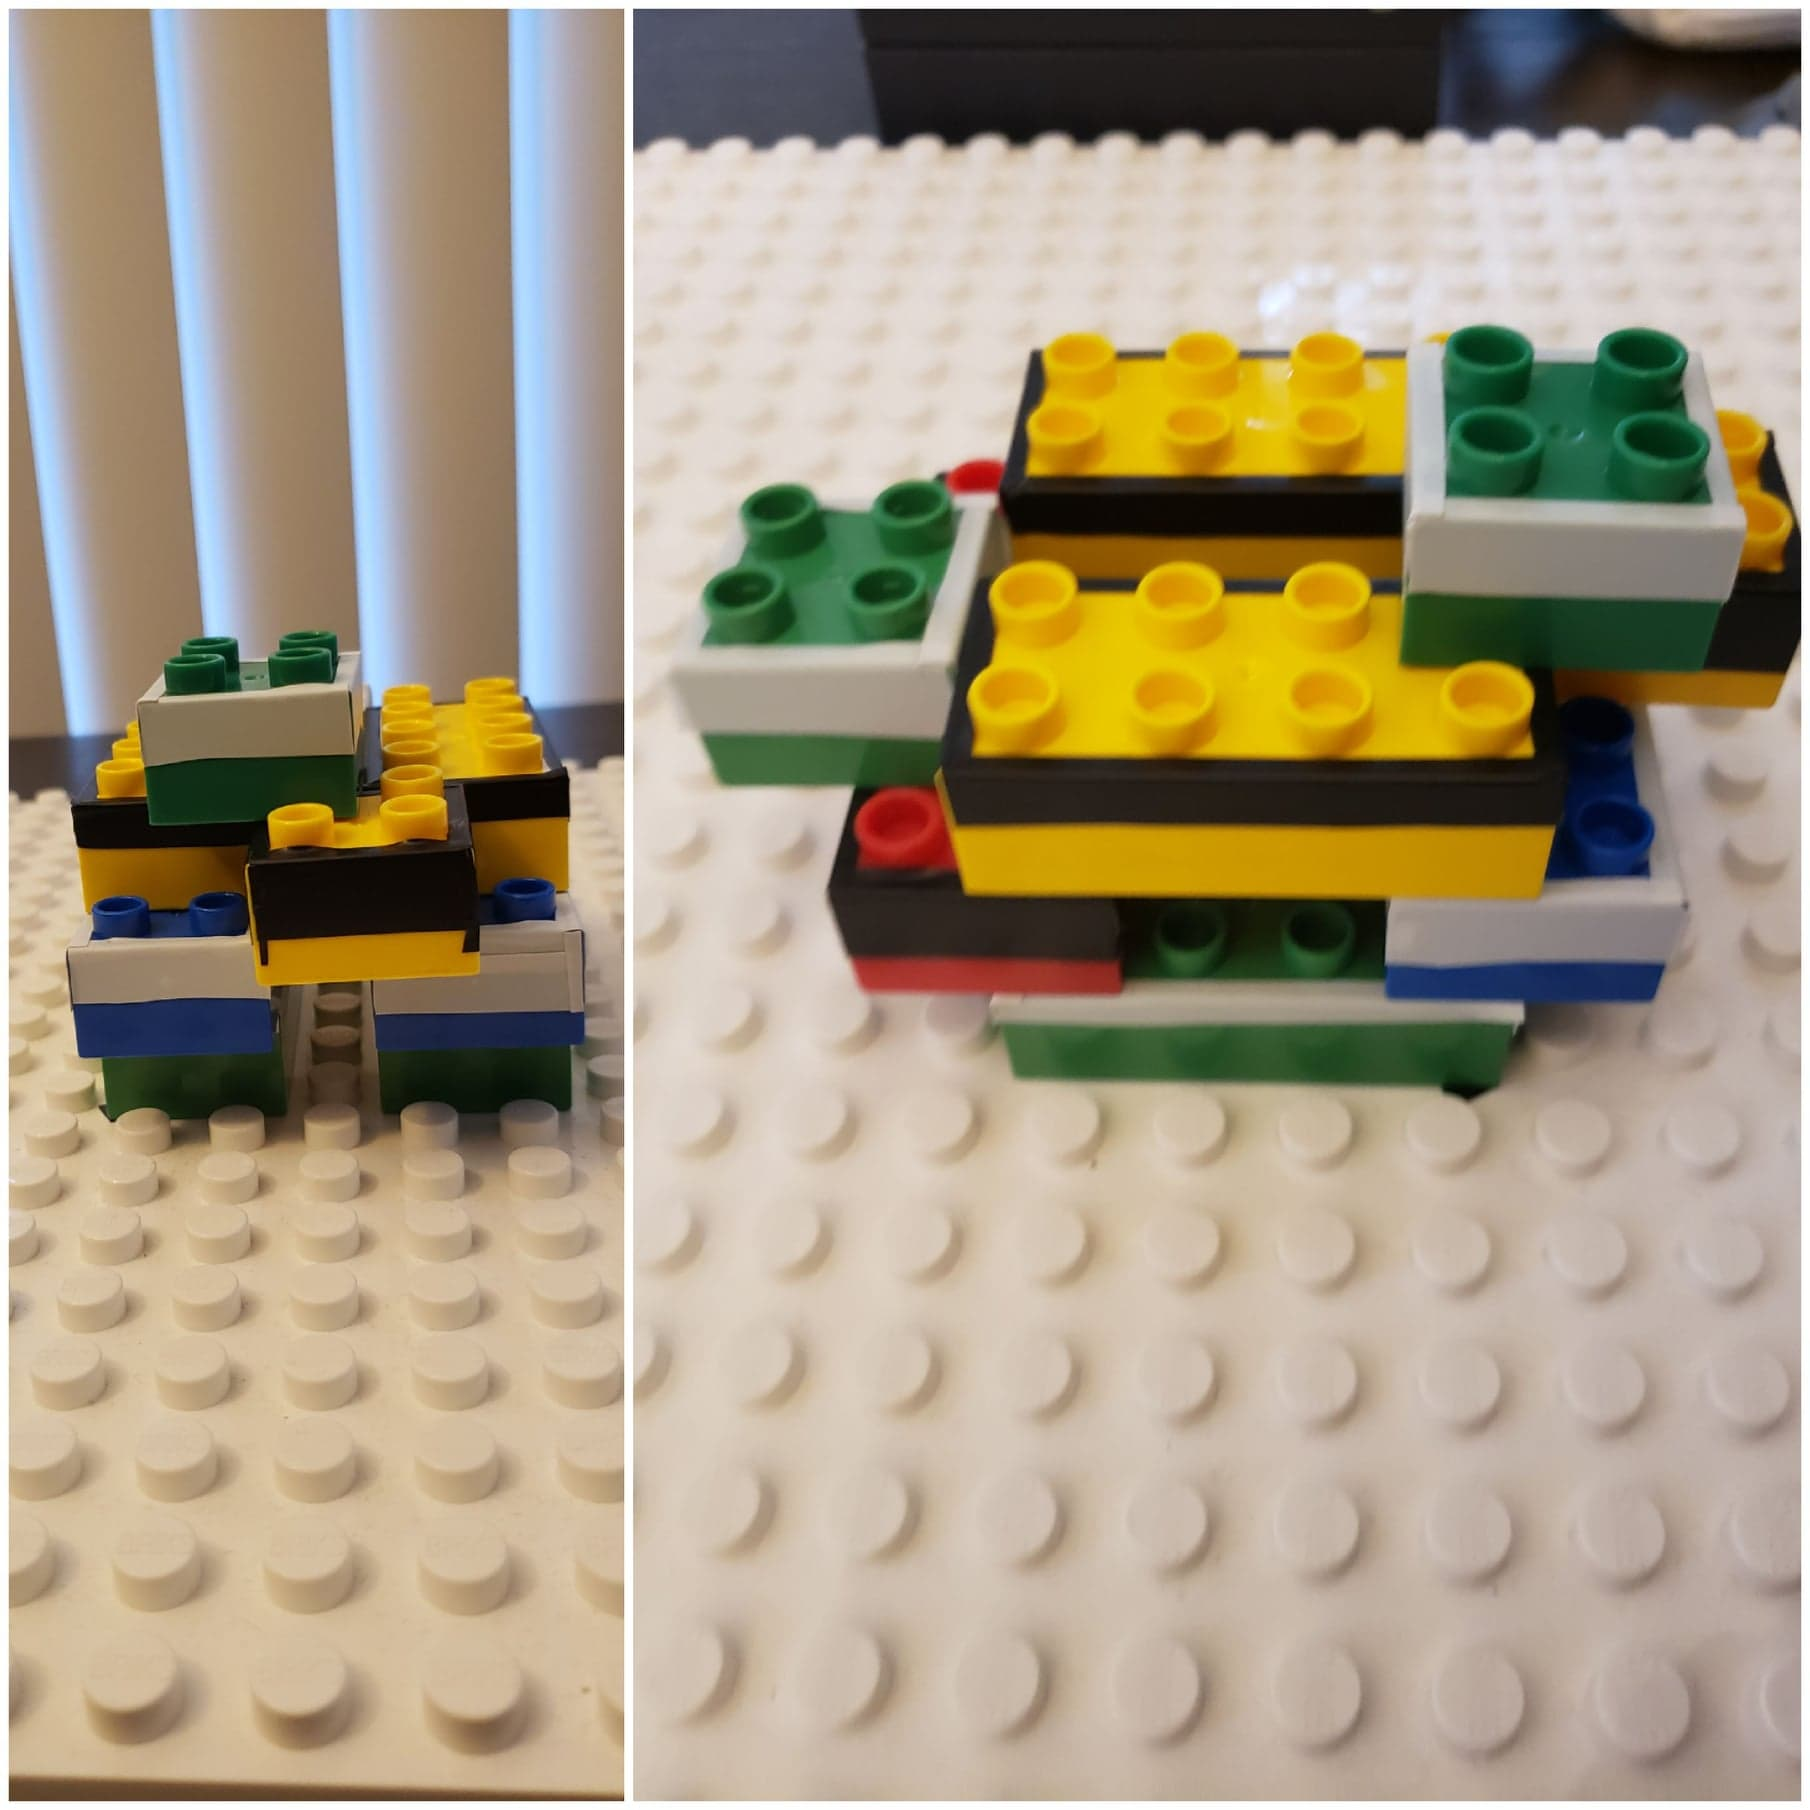
\includegraphics[width=0.8\linewidth]{figures/e6.jpg}
       
       \caption[{}]{\label{fig:fig_3-7d}}
    \end{subfigure}
    \begin{subfigure}{0.5\textwidth}
       \centering
    %   \includegraphics[width=\textwidth,height=\textheight,keepaspectratio]{fig_3-3}
       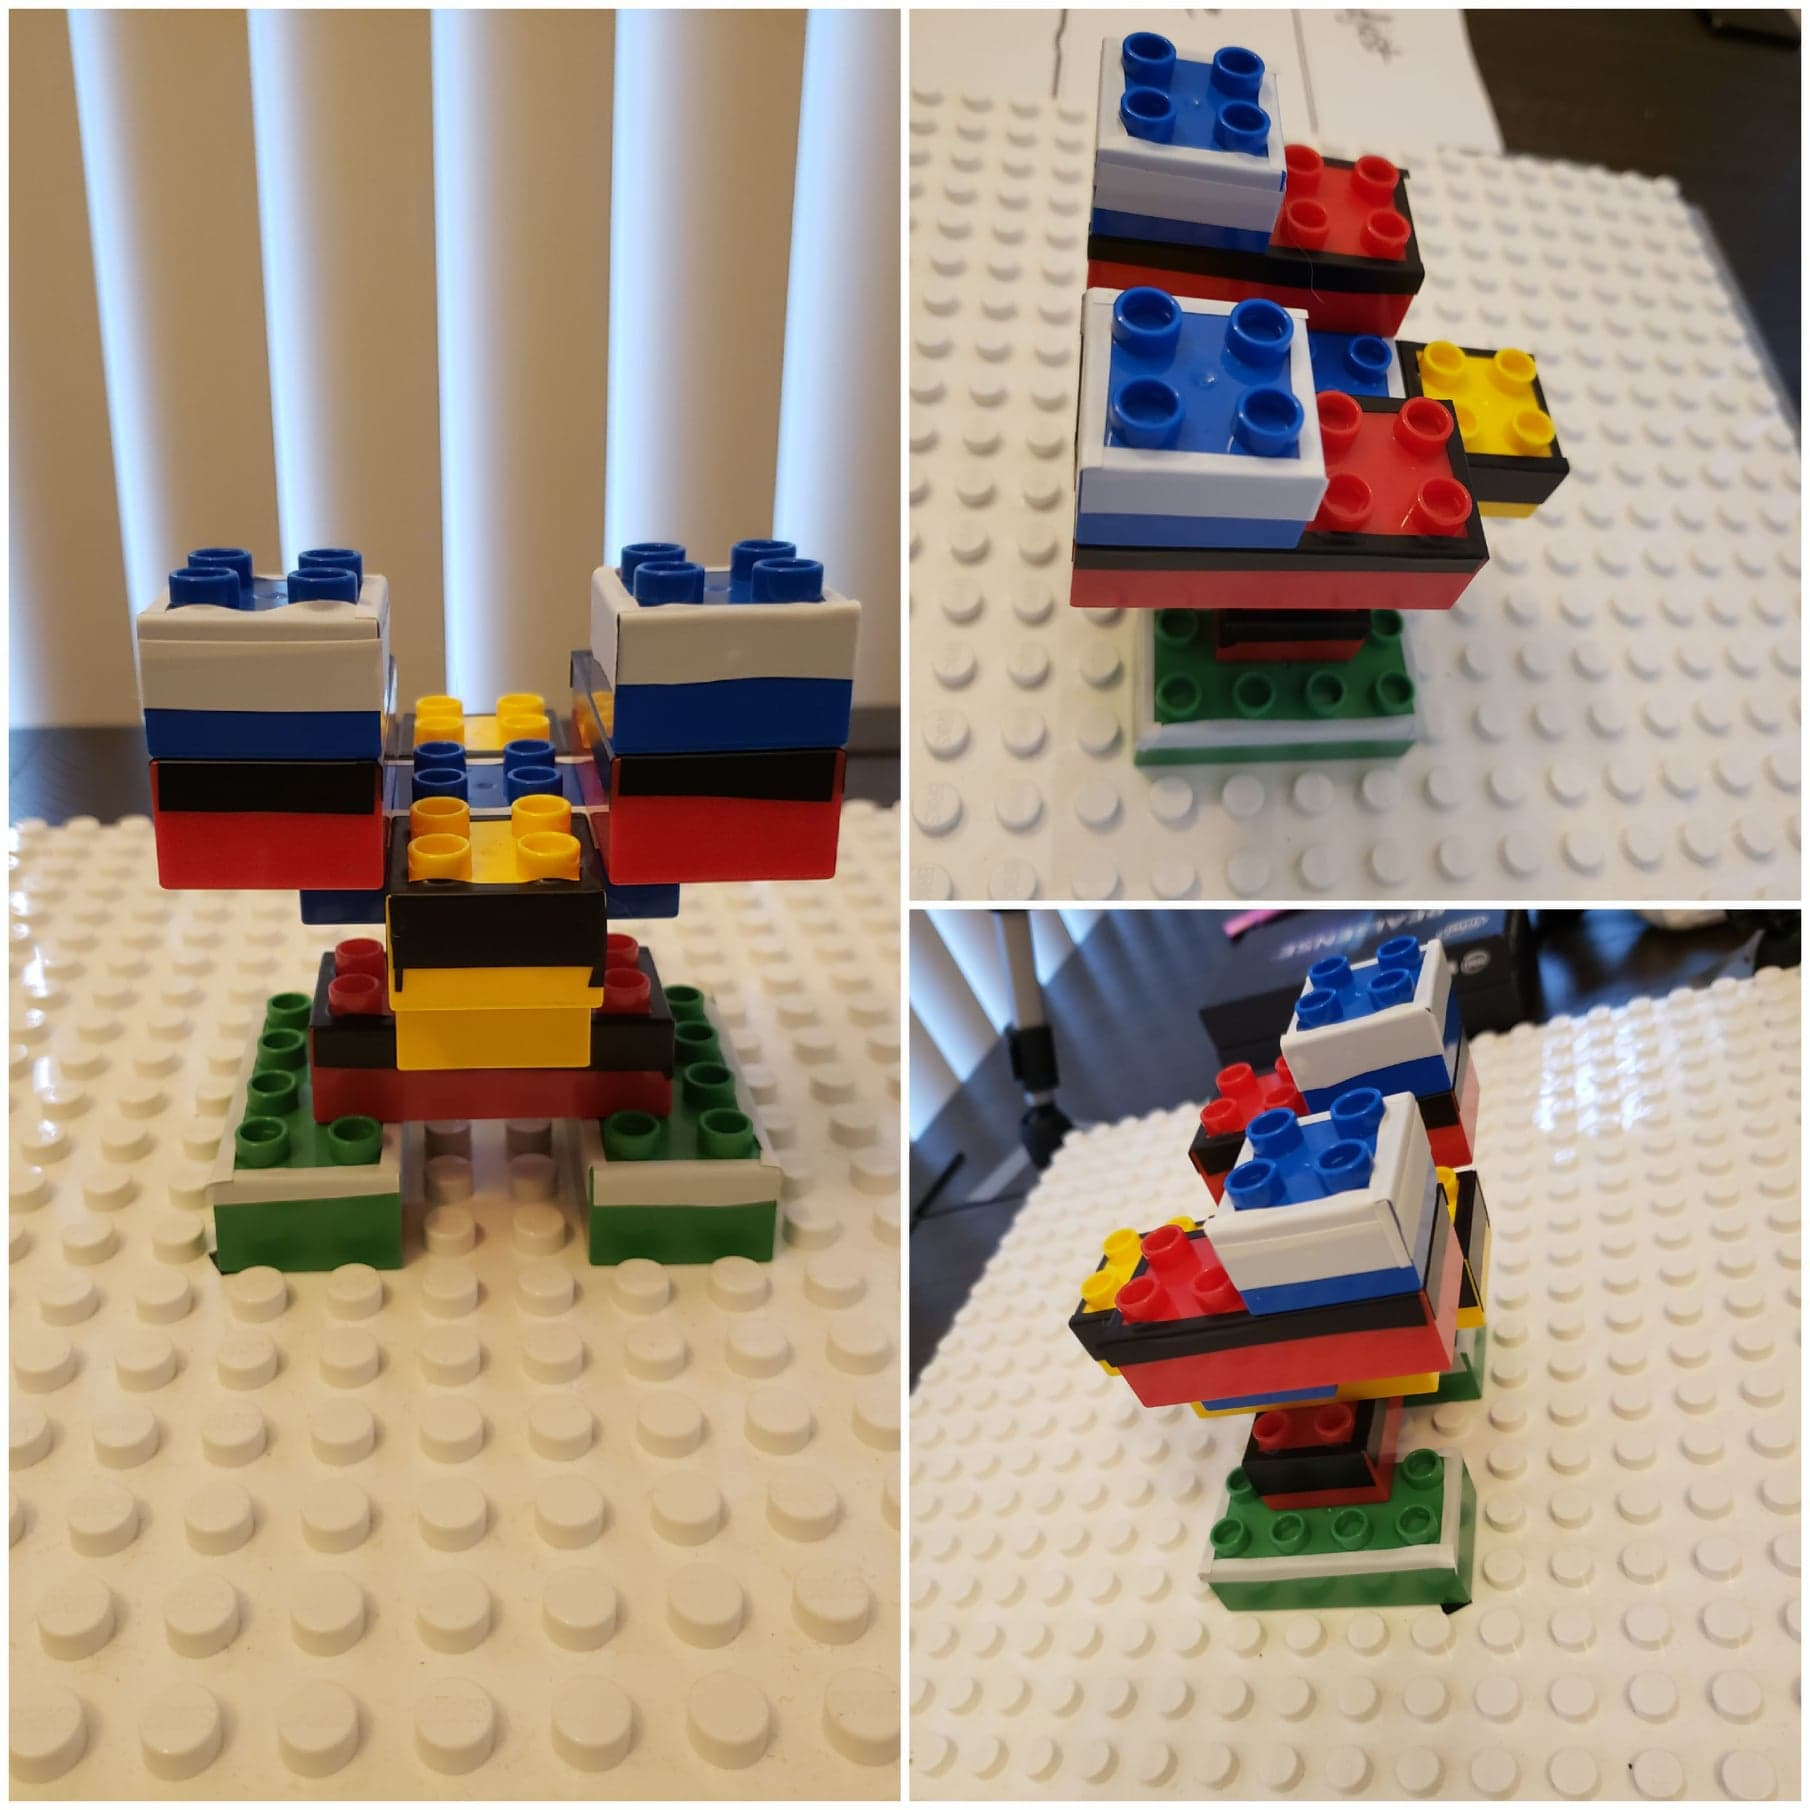
\includegraphics[width=0.8\linewidth]{figures/e7.jpg}
      
       \caption[{}]{ \label{fig:fig_3-7e}}
    \end{subfigure}
    \caption[{Complex 3D structures}]{Complex structures successfully completed in both learning and teaching modes. Picture on left is front view and picture(s) on right are side view(s).}
   \label{fig:fig_3-7}
\end{figure}
\subsect{Evaluation and Limitations}
The system runs on Ubuntu (in dual boot with windows) in real-time on a laptop PC with 5-core 2.3 GHz Intel\textsuperscript\textregistered{} processor. It takes about 2-5 seconds to update the model when required. There is no lag in the system. The system works fairly well in most of the cases. Some simple structures, which can be recreated by looking at only one view, were successfully completed by us in the learning mode and tested in teaching mode as shown in figure \ref{fig:fig_3-6}. Some complex structures were also tested by the system are shown in figure \ref{fig:fig_3-7}. These complex structures requires at least pictures of 2 views to recreate. These structures were successfully detected and stored by our system. Various random structures were also tried to look for possible errors and limitations of the system. Some of the errors and limitations observed are:

\begin{enumerate}
    \item Occlusion: Since only one camera is used to track the workspace, if the block to be added or removed is not fully seen by the camera, it will go undetected and cause errors as shown in figure \ref{fig:fig_3-4}. Using multiple RGB-D streams from various cameras can eradicate this issue. 
    \item Confusion: As explained above, the error in \textbf{.z} is fixed by intuitively lowering the level until it overlaps at least one block underneath it. This fixes the \textbf{.z} for time being for that block but when new block of same shape (or appearing to be of same shape) is requested to be added, the overestimated z would stop at a level higher than before thus re-adding that object thinking that it is a new object at upper level as shown in figure \ref{fig:fig_3-5}. Using better method for estimating error in depth because of oblique camera or using multiple RGB-D cameras can help reduce this error.
    \item Due to changes in light source, sometimes, HSV based color detection is faulty but it can be fixed by fixing the light source.
    \item The whole 3D structure is grounded on a base, thus not allowing the user to move it around in space. 
    \item The blocks have been taped on edges (as seen in figures) to assist color segmentation and enable differentiation of same colored blocks. The boundaries allow different shapes and multiple blocks of similar characteristics to be used for block building. 
\end{enumerate}
\begin{figure}[h]
   \centering
%   \includegraphics[width=\textwidth,height=\textheight,keepaspectratio]{fig_3-4}
   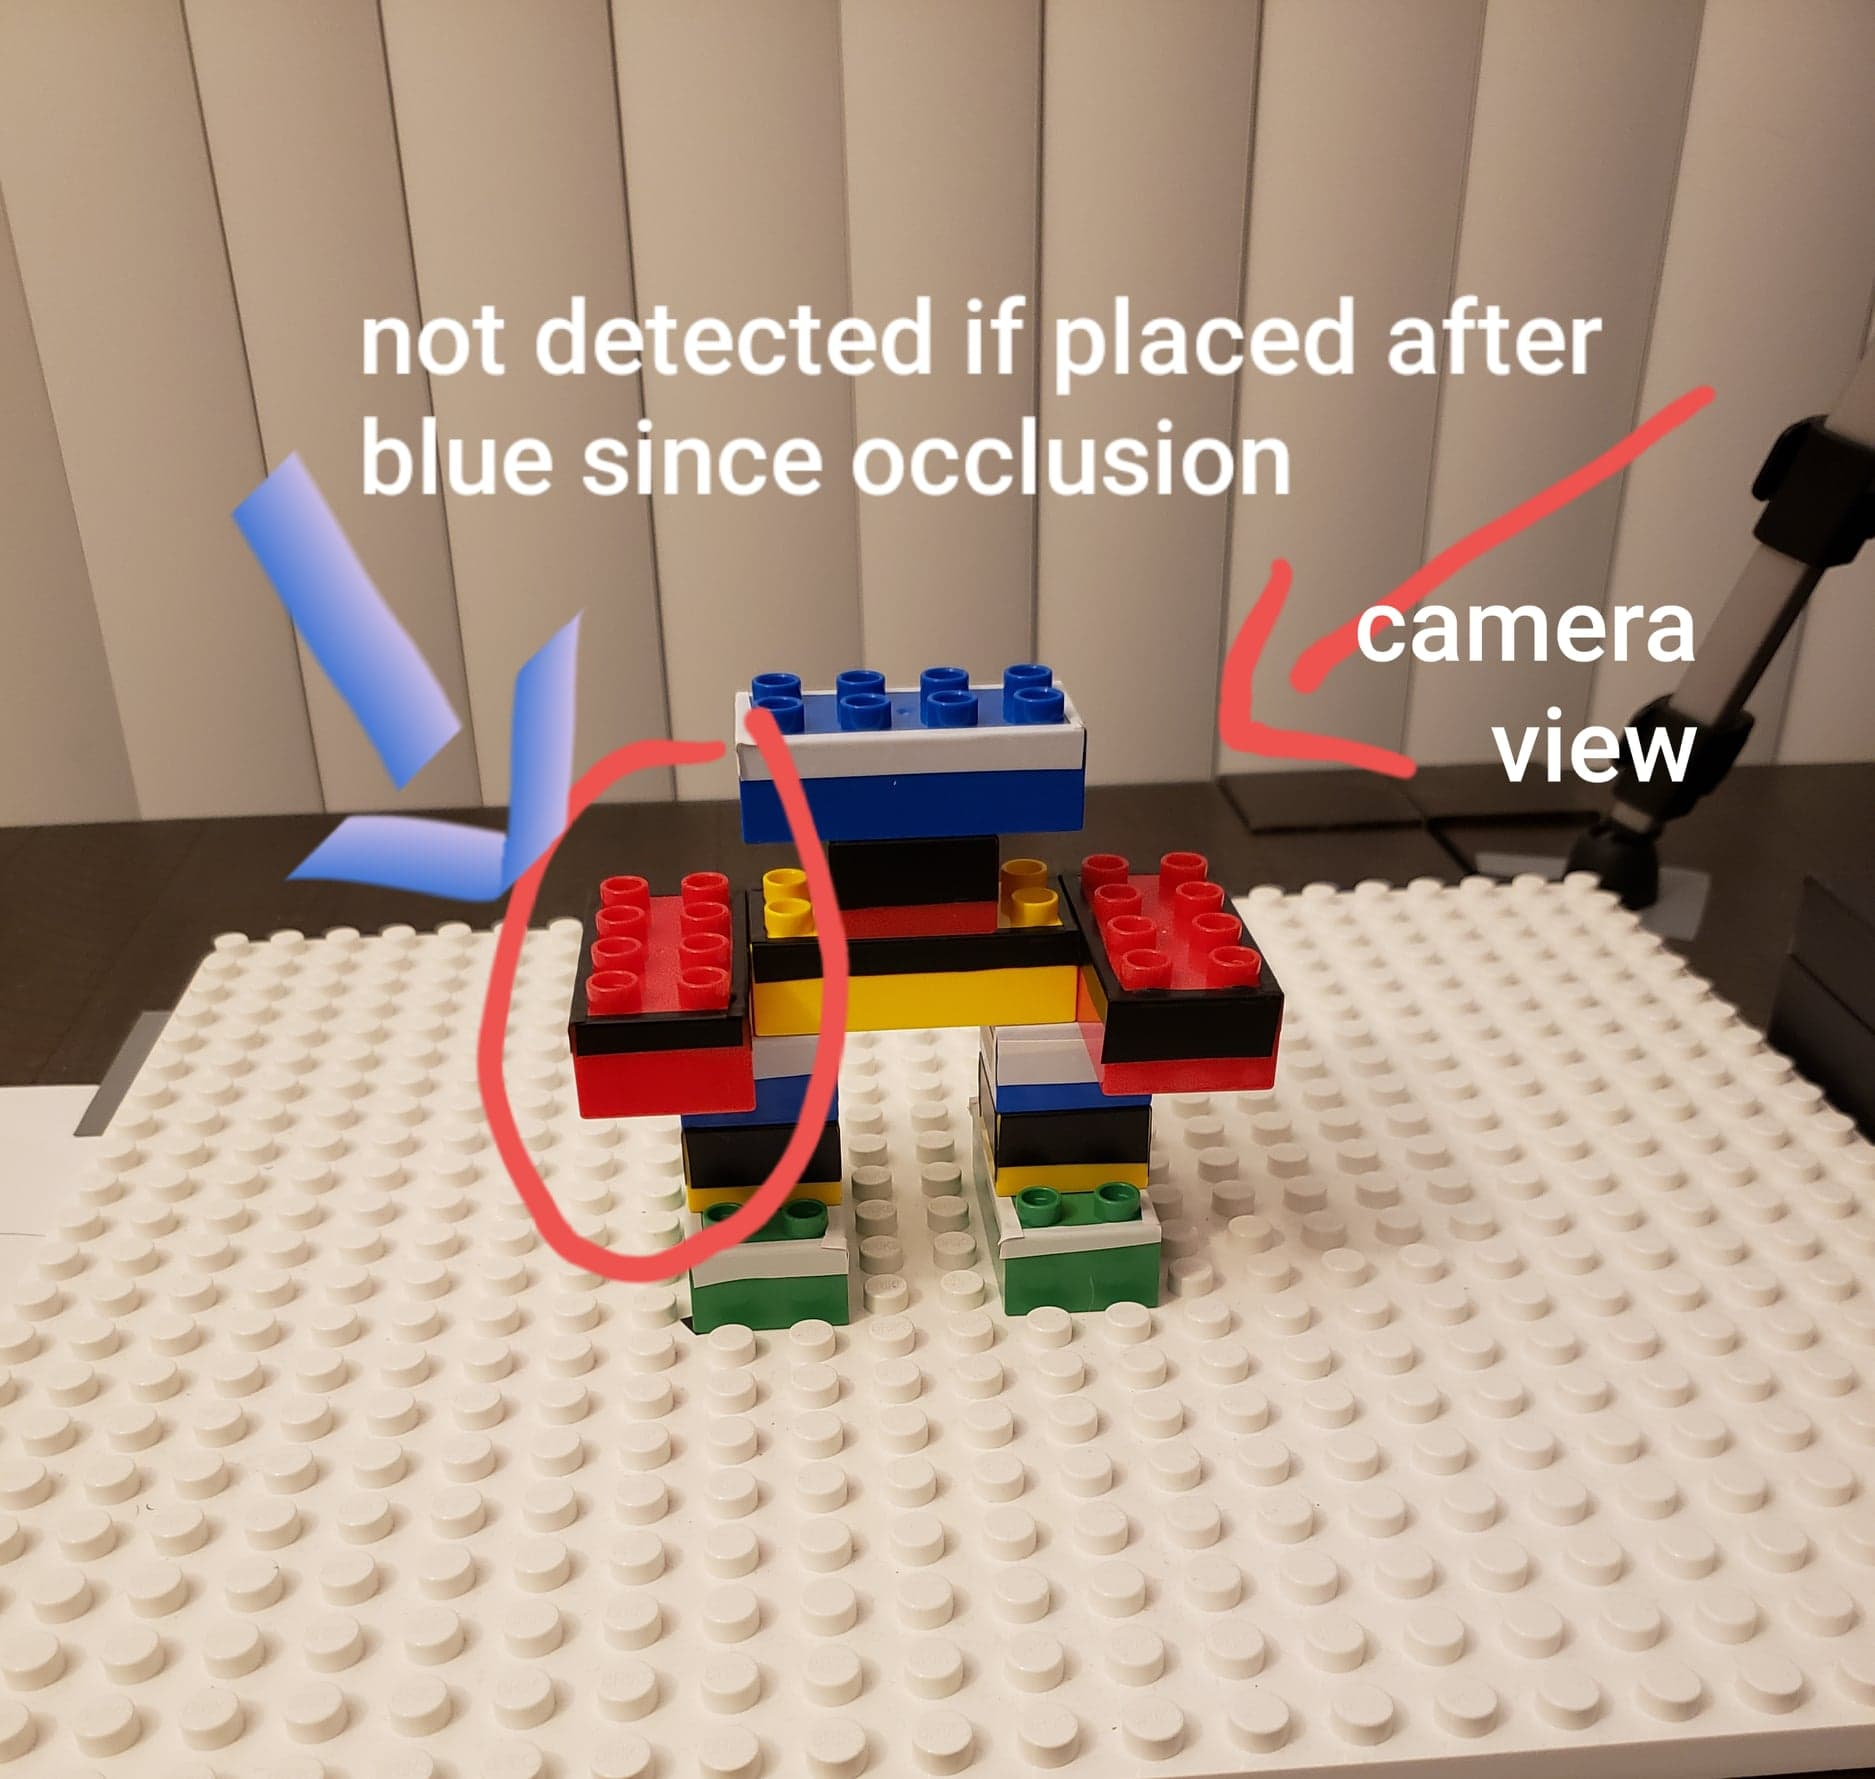
\includegraphics[scale=0.2]{figures/occlusion.jpg}
   \caption[{Example of occlusion}]{Example of occlusion: The circled $2 \times 4$ red block on level 4 will not be detected if placed after the $2 \times 4$ blue block on level 6 because the camera cannot see it fully}
   \label{fig:fig_3-4}
\end{figure}

% Figure 3-5
\begin{figure}[h]
   \centering
%   \includegraphics[width=\textwidth,height=\textheight,keepaspectratio]{fig_3-5}
   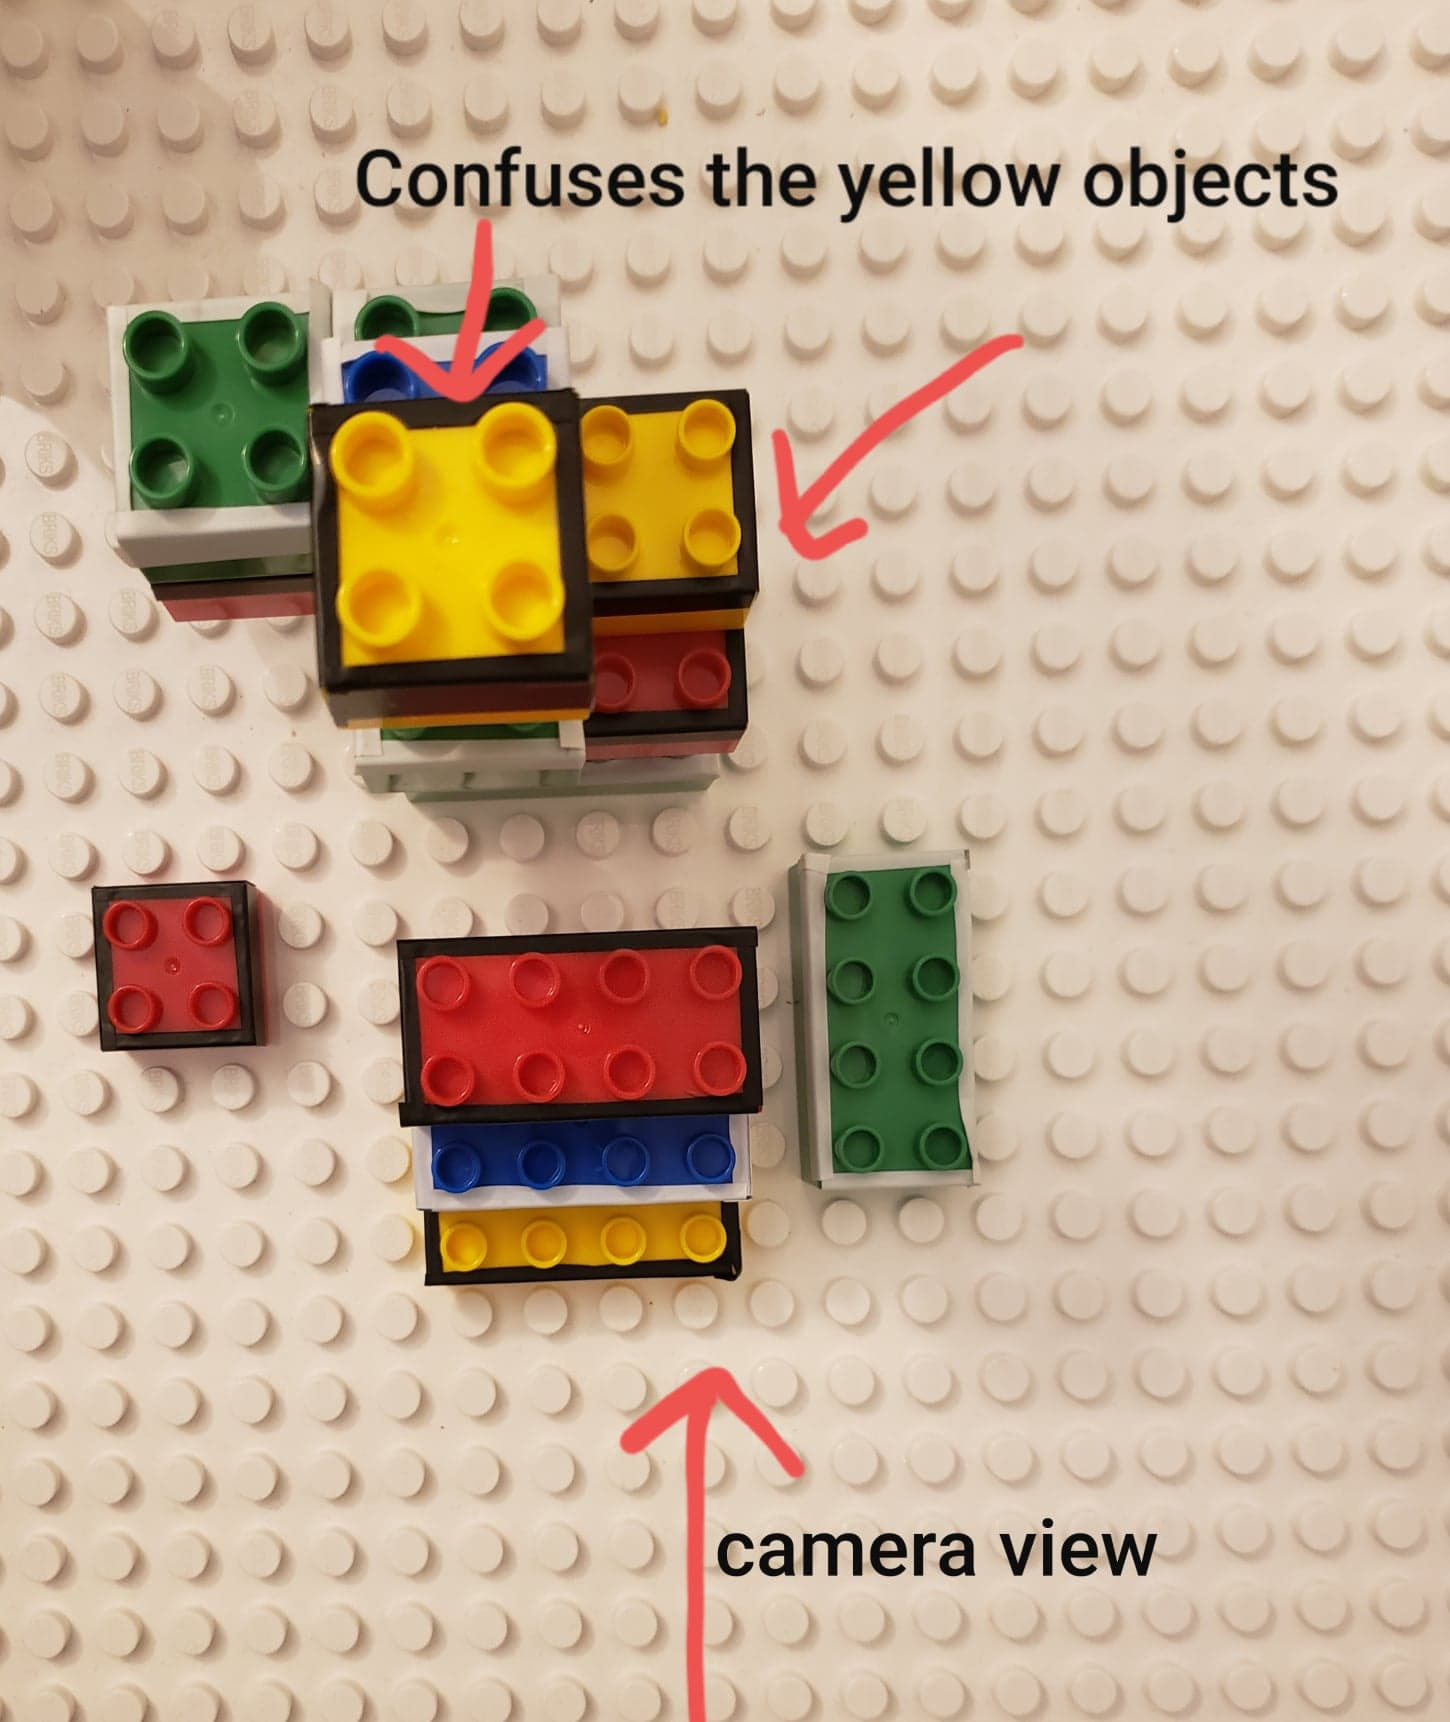
\includegraphics[scale=0.2]{figures/confusion.jpg}
   \caption[{Example of confusion}]{Example of confusion: The $2 \times 4$ yellow block at lower level is mistakenly added as a $2 \time 2$ yellow block because it appears to be a $2 \times 2$, even before the user placed the top level $2 \times 2$ yellow block because the rectangle at $\textbf{.z}=4$ originally had been assigned $\textbf{.z} > 4$ and it was corrected to 4. Thus, now the visible portion of lower level yellow block appears to be a new block added at level 5 ($\textbf{.z} = 5$)}
   \label{fig:fig_3-5}
\end{figure}
Despite these limitations, the proposed perception module has some advantages over similar systems. It is able to use two different shapes unlike in Gupta and colleagues' system \parencite{gupta2012duplotrack} which uses only $2 \times 4$ blocks. It can be extended to other shapes e.g. $1 \times 2$ blocks easily. Also, it is able to use multiple blocks of 4 colors of 2 shapes unlike Jones and colleagues' system \parencite{jones2019toward}  which uses only one block of each shape ($2 \times 4$ and $2 \times 2$) and 4 colors (total of 8 blocks). Our model representation is robust and efficient. Such simple representation enables us to track an assembly which has multiple paths towards correct solution. We are able to get all possible correct next actions and all possible removable items at any step. It is not a step by step process strictly since there can be multiple correct actions at any step unlike step by step guided system proposed by Gupta and colleagues \parencite{gupta2012duplotrack}. Also, we use a reference block for defining (0,0) for xy-coordinates, thus, the learnt graphs stay valid even if the reference block is moved at the start of each 3D building task.  


%\subsect{Applications}


\sect{Feedback}
Second module of the system is providing feedback in teaching mode to help the user finish the 3D block building task at hand. Feedback system receives various types of errors in new block from each possible correct block. Based on the number of possible correct blocks, number of errors from each possible correct block and type of errors, the error on which the robot must give feedback is decided. Following rules are followed:
\begin{enumerate}
    \item If there is a possible correct block with 0 errors from new block, a brief statement confirming the correctness of the action and suggesting to continue is provided. We call these statements \emph{continuers}. 
    \item If there is only one possible correct block and there is only one type of error, that error is selected by default.
    \item If there are two or more errors with respect to the only possible correct block, following priority is considered while choosing the error to respond to:\\
    Error in: Shape $>$ Color $>$ Orientation $>$ Level $>$ Position
    \item If there are two or more errors with respect to two or more possible correct blocks. The possible correct block with which there are least errors is selected and the error priority is decided as following:\\
    Error in: Shape $>$ Color $>$ Orientation $>$ Level $>$ Position
\end{enumerate}
Two main questions to answer are: When to give feedback and what would the feedback statement say. As far as \emph{When} is concerned, for this exploratory study we provide feedback to user every time a mistake is made. Although due to delays in execution of robot behaviour continuers might be skipped every now and then. To answer the second question, we inspire from feedback strategies that are summarized in table \ref{tab:tab_2-1}. Table \ref{tab:tab_3-1} shows the design of feedback statements that is published to a rostopic for robot to convey to the user. 
\begin{table}[]
    \centering
\begin{tabular}{ | m{2cm} | m{3cm}| m{8cm} | } 
\hline
\textbf{Error type} & \textbf{Feedback Type} (refer to table \ref{tab:tab_2-1}) & \textbf{Feedback Statement} \\ 
\hline
\multirow{4}{4em}{Shape or Color}  & 8a. & The shape/color should be \_ instead of \_ \\ \cline{2-3}
& 1. 7c. 8b. & Hmm, are you sure you need a \_ here? \\ \cline{2-3}
& 3. 4. 7c. & So, if this is a \_ , what should be the next step?\\ \cline{2-3}
& 7c. 8b. & What if we try a \_ instead?\\ \cline{2-3}
\hline
\multirow{3}{4em}{Orientation}  & 8a. & The orientation is wrong. You need to rotate the block \\ \cline{2-3}
& 1. 8b. & Umm. Does this orientation looks right to you? \\\cline{2-3}
& 7d. 7h. 8b.  & What if we rotated the block, Wouldn't it look better? \\
\hline
\multirow{3}{4em}{Level}  & 8a. & The level is wrong. Move the block to upper/lower level. \\ \cline{2-3}
& 3. 8b. & What if we moved the block to upper/lower layer?\\ \cline{2-3}
& 7c. 8b. & Hmm, would you check if the block is at the right height?\\ 
\hline
\multirow{4}{4em}{Position}  & 8a. & The position is wrong, Move the block \_.  \\ \cline{2-3}
& 1. & I think the block is not at the right position. Would you try fixing it?\\ \cline{2-3}
& 7d. 7h. & Hmm, Let's try moving this block around a little bit to see if we get it right.\\ \cline{2-3}
& 3. 4. 7c. & If this is the right position for this block, think what would be on top of it?\\ 
\hline
For all  & 7d. & Let's look at the given picture to see if this looks alright. \\ 
\hline
No error & 2 & One of following \emph{continuers} with a nod: Go on. Continue. Hmm. Good. Right. \\
\hline
\end{tabular}
  \caption{Feedback statements based on selected error and inspired from literature as summarized in table \ref{tab:tab_2-1}.}
    \label{tab:tab_3-1}
\end{table}

\sect{Robot Behaviour}
The third and last module of the system is introducing somewhat life-like movements in the robot. The robot we are using is Maki, a 3D printed robot with 7 servos and controlled using arbotix\_m controller as seen in the setup (figure \ref{fig:fig_1-1}. Maki provides verbal feedback when a mistake is made by the user. Microsoft\textsuperscript\textregistered{} Azure text-to-speech service is used to convert the feedback statement into human-like voice. Apart from speech, we program Maki to nod slightly to acknowledge the correct actions of user along with continuers such as \emph{go on}, \emph{continue} and \emph{good} etc. This is to remind user of its presence and keep the user engaged. We have implemented another robot behaviour known as referential gaze: In idle state, Maki looks at the user. When the user makes a mistake, the robot looks towards the play area as if it is analyzing the workspace, narrates feedback to the user and then looks back towards the user to take requisite action to correct the mistake made.
















%\printbibliography[title={References}]
%\end{refsection}
%
%\begin{refsection}[myrefs.bib]
\chapter{Exploratory Study}
\label{chap:four}
%\newpage

% Introduction

We conducted an exploratory study to analyze our system. Various aspects of the study are explained below:
\sect{Participant}
Our participant was an elementary-aged female student. She is currently in fourth grade. Her past experience with technology in the classroom is limited to using tablet computers. She has interacted with Maki (the robot) previously for a different pilot study.
\sect{Task}
For the sake of this exploratory study simple structures as shown in \ref{fig:fig_3-6} are selected as 3D block building tasks. The complex structures(figure \ref{fig:fig_3-7}) require at least 2 different views to be completed and after initial interaction with the participant, we found that these structures are too complex for her to follow even with feedback from Maki. Thus, we use the simple structures for this study.
\sect{Procedure}
As seen in figure \ref{fig:fig_1-1}, the setting of tasks consisted of Maki the Robot, playground with Lego\textsuperscript\textregistered{} blocks, play area and control boxes, a camera mounted on a tripod stand, an iPad for displaying the target 3D block structure and the participant seated on a chair. \\
First of all, the participant is seated. She is presented with a 3D structure to build with blocks as a pre-test for the study. Pre-test is administered to develop an understanding of her existing knowledge of block building. The task given as pre-test is shown in figure \ref{fig:fig_3-6a}. The experimenter explains the functionality of box controls and play area, and asks the participant to build the given structure . Participant is aware of the functionality partially because of similar interaction in early stages of this project. This prior interaction was carried out to understand if the proposed playground with control boxes is understandable by school-going kids and to analyze the complexity of 3D block building tasks that can be targeted towards elementary-aged students. \\
After pre-test, Maki introduces himself and explains what the participant will be doing today and prompts her to start her first task, as shown in figure \ref{fig:fig_3-6b}. During the task, Maki provides feedback whenever a mistake is made. On correct actions, Maki narrates statements encouraging to continue or affirming correctness of action e.g. \emph{Okay. Good. Go on. Continue.} etc. so that the participant does not neglect the robot in the process in case she is not making mistakes for long time. The run ends when she successfully completes her task. Maki congratulates her on success and she is asked to take a break before next task with a different target structure. Maki welcomes her back to each next task and prompts her to start the task following same instructions. Four more structures ( figure \ref{fig:fig_3-6c}, \ref{fig:fig_3-6d}, \ref{fig:fig_3-6e} and \ref{fig:fig_3-6f}) are done in next tasks. After all the tasks, a post-test similar to pre-test but with different target structure as shown in figure \ref{fig:fig_3-6g} is taken. After last task, a post-study interview is conducted in which the experimenter asks the participant about her experience with the system and Maki, whether she found Maki to be helpful or bothersome, whether she would trust Maki to guide her in learning about the given task and if she felt encouraged to continue the task. 

\sect{Measurements}
We collect data through three main sources: \textit{pre and post test}, \textit{post- study interview} and \textit{video analysis}. The video is viewed by the author. Rudimentary qualitative analysis is done on the video data. 

% Results
% Discussion
\sect{Results and Discussion}
We analyzed the pre and post test, videos from 5 tasks and post-study interview qualitatively. Results from these three sources of data are discussed here:
\subsect{Pre and Post-test}
The participant successfully completed both pre-test and post-test task. Both tasks were of similar complexity. Over all outcome for both the tasks was correct but for the pre-test the participant used remove control once self-correcting her mistake. However, in the post-test, she did not make any mistake and only used add control. Also during the pre-test task, experimenter had to explain the functionality of adjust and remove blocks once again. Since there was only one session and tests ended up being rather simple, nothing can be concluded about learning gain from one session qualitatively. \\
\subsect{Video Analysis}
Many observations were made by the viewer of videos of interaction with Maki. The main observations over the 5 tasks are summarized as under: 
\begin{enumerate}
    \item She looks at Maki when he communicates with her for introduction of task, feedback statements and robot actions e.g. nodding and referential gaze. But as she goes further into the session, time of her eye contact with Maki reduces while he is repeating the same statements at start and end of each task. But, in the last task, the ending statement was different since Maki tells her about end of her session with him and bids her goodbye. At the start of this ending statement, she was looking down but as soon as the statement was different from the previous ending statements, she turned her gaze towards Maki to process new information. It is interesting to note that she stopped looking at Maki and stareted listening passively when he said predictable and repetitive statements but as soon as he narrated new information, she paid full attention to Maki. 
    \item She follows what Maki is asking or suggesting her to do. For instance, during intro statement when Maki says to look at the screen for picture of target structure, she looks at the screen. When Maki narrates continuers like \emph{Go on, continue} etc. she moves on trusting Maki's suggestion that she is correct. She considered \emph{nodding} of Maki as confirmation of her being correct as well.
    \item She looks at robot after every action for confirmation if she did it right or not. Sometimes, she would skip looking at robot but as soon as the robot nods and says a continuer, she would look at robot and move on. Sometimes if robot would not respond to her action, she would wait a couple seconds looking at robot for a response to her action. She would move on if she did not get a confirmation assuming that she did it right. This suggests that if you provide frequent feedback, the user can get accustomed to it and wait for the feedback. Also, it is interesting to note that the lack of feedback made the participant assume she was doing alright. She trusted Maki to point out her mistake. 
    \item During task 4, even though Maki was congratulating her on her successful completion of task, she was looking at the picture of target structure. She mentioned it to the experimenter that she thought there was still one more block left to be added in the structure.  This might be because of few glitches in the same task. The system made a wrong detection because she took too much time to fix the block and it got detected midway and robot hinted to look at the picture again to see if it is alright. While adjusting again, the robot mentioned that the position is wrong and asked to move the block upwards. This confused the participant since she was placing the block at right place. Experimenter interfered and suggested her to adjust the block again. After adjust action, Maki nodded and suggested to move on since system was able to correct its wrong detection during adjust action. This shows that the participant did not blindly trust Maki and since it made a mistake earlier in the same task, she was skeptical of Maki congratulating her on completion of her task and wanted to make sure for herself.
    \item Apart from task 3, figure \ref{fig:fig_3-6d}, she did not make mistake in any other task suggesting that the simple tasks (figure \ref{fig:fig_3-6}) are easier to do for kids of her age group.
    \item Task 3 mistakes: She made 2 mistakes in task 3. The target structure is shown in figure \ref{fig:fig_3-6d}. The first mistake was that she used a yellow rectangular block instead of a square one at fourth step. As it is clear from the picture of target structure, the structure has a possible confusion i.e. \emph{a rectangle of yellow} instead of \emph{a square of yellow and a square of blue}  at level 2. Maki responded saying \emph{Are you sure you need a rectangle here?}. She inferred that the hidden block is blue square not continued yellow rectangular block and she fixed her mistake by removing the yellow rectangular block and replacing it with two square blocks of yellow and blue color. the second mistake was that she placed the blue rectangular block at level 3 before the green square block at the level 2 so, robot pointed out that the shape should be a square instead of a rectangle. , this feedback statement was not very clear i.e. the blue rectangular block at level 3 is the correct block but green square needs to be added at level 2 before that, she corrected her mistake anyways. This implies that merely pointing out that a mistake has occurred nudged the participant to correct herself. Thus, it is safe to say that the participant received feedback from the robot positively and self-corrected her mistakes.
\end{enumerate}
\subsect{Post-study Interview}
To support observations from the video analysis, we conducted a post-study interview. We asked the participant questions about her overall experience, her perception of Maki, her comfortability with the setup, her feelings about Maki's appearance and behaviour. This interview revealed lot of interesting information. Some of the remarks from the participant and our interpretation of these remarks are detailed below:
\begin{enumerate}
    \item \textbf{Fun and engaged}: She thought that the over all experience was fun despite some of the bugs and wrong detections. She also said that she would enjoy more sessions with Maki because it was fun. She expressed that if she had to do the tasks by herself, it would be boring.
    \item \textbf{Fascination}: She was fascinated with Maki since she does not work with robots usually so she thought it was fun. She would prefer working on similar tasks with a robot over a human because she finds that humans can be boring sometimes and \emph{humans just do not work with other humans}.
    \item \textbf{Helpfulness}: She perceived Maki to be cool and helpful because she noticed that whenever she was correct, the robot nodded and said \emph{Go on, continue} etc. and whenever she was wrong, he helped her with a hint. She expressed that she would like more sessions with Maki and she learnt a bit about block building task and she will be better at it now. The session boasted her confidence in her ability to work on similar tasks. She expressed that without Maki it would not be easy to complete the tasks.
    \item \textbf{Teacher vs Peer}: She found Maki to be acting like a friend when he gave hints to help her through the task but she thought of Maki as a teacher when he told her if she was wrong or right. This suggests that direct feedback e.g. using the word \emph{wrong} creates impression of Maki as a teacher while helpful hints created more of a friend-like personality. 
    \item \textbf{Trust} She trusted the robot but not blindly. She trusted Maki when he provided feedback on her mistakes. At some point, she thought she was right and the robot was wrong. Even if the robot made mistakes, she was okay with it because Maki was not a human and she could trust it because it was right sometimes. Maki's mistakes in providing feedback would not stop her from working on further sessions with Maki. 
    \item \textbf{Scaffolding and self-regulation}: When Maki used the word \emph{wrong}, her emotions were hurt. She said it made her sad but when he acted in a friend-like manner and gave suggestions without using the word wrong, she felt better and she knew that she can get her mistake right again. She found Maki to not judge her for her mistakes unlike humans. This is an interesting find that using softer words to suggest mistakes resulted in the participant scaffolding and self-regulating her learning process. 
    \item \textbf{Clarity of feedback}: She found Maki's remarks to be loud and clear. She understood her mistakes from feedback statements and was able to fix those.
    \item \textbf{Frequency of feedback}: The participant was asked if she found Maki to be excessively talkative, annoying and interrupting her. She said that this was not the case. In fact, whenever Maki would not respond she was concerned that he should have said something. 
    \item \textbf{Appearance and robot behaviour}: The loud noise made by robot while moving its head was scary but not in the sense that it would harm her since Maki has no limbs. Whenever Maki moved, she was looking forward to hear something from him. It is interesting to note that robot behaviour such as node and referential gaze are interpreted as robot's intent to communicate with the participant. The participant was also able to distinguish the meaning of nodding (correct action) and referential gaze (mistake made). Maki's voice was perceived neutral and non-expressive. In her words, it was lacking highs and lows. He did not sound excited or if anything mattered to him. She was of the opinion that Maki should at least be expressive. She did not expect Maki to have emotions as such. 
\end{enumerate}
\sect{Design Implications and Suggested Improvements}
This exploratory study has helped understand better effectiveness and drawbacks of our perception system, feedback strategy and robot behaviour. It has shed light on the potential of robot assisted 3D block building to augment spatial visualization skills in elementary-aged students using implicit feedback strategies to suggest mistakes made in place of explicit corrective feedback. 3D block building task is found to be more engaging and interesting in the presence of the robot. The robot assisted the participant to correct her mistakes through frequent feedback. The participant anticipated feedback from the robot after every action and it concerned her if the robot did not respond. Implicit feedback such as suggestion, hints, giving second chance to correct herself and redirecting created positive emotions such as confidence in the participant and helped her self-regulate her learning process. Implicit feedback had clarity regardless of not putting the exact mistake in words. Using strong words such as \emph{wrong} had a negative impact on the participant thus, suggesting explicit corrective feedback can harm self-confidence. The robot was able to build some level of trust despite a couple of mistakes on its part. The robot was perceived as a teacher when it communicated whether the action of the participant is right or wrong whereas it was considered a friend when it gave suggestions and hints to assist the participant. Robot's behaviour i.e. nodding and referential gaze were easily distinguishable. New statements or actions by robot would get the participant's full attention whereas repetitive statements caused participant to go into passive listening.\\
This exploratory study will enable us create a framework for a detailed study to evaluate effectiveness of our improved system and study design. Following are the suggested improvements that will enable us in resolving certain issues of our system and get it ready to launch a full-fledged study to analyze learning gain, self-regulation and scaffolding ability of students and their perception of a robot tutor in one-on-one session while conducting a 3D block building task to augment spatial visualization:
\begin{enumerate}
    \item Two factors need to be part of elaborated study: Type of feedback (implicit vs explicit) and frequency of feedback (when to give feedback?). Although, given the results from this study implicit indication of mistake implied better ability to self-regulate and friendliness and likability of the robot, data is too less to make a conclusion. Similarly, the participant preferred frequent feedback in this study but nothing can be said about its effects on learning gain. It is possible that interrupting frequently to provide feedback might make the user too dependent on the robot to figure out when and what mistake is made. Nothing conclusive can be said about these two factors with limited interaction data. Although, these two factors need to be explored further in detail. 
    \item The perception system needs to be improved to increase credibility of feedback provided by the robot.
    \item To be able to evaluate learning gains, ability to scaffold and self-regulate, it would be better to have multiple sessions over longer period of time since spatial visualization skills are hard to quantify in one session. Also, these skills improve over time and we are interested in long-term effects of feedback strategies and robot assistance on spatial visualization. 
    \item Designing the 3D target structures needs to be guided by experts in the field e.g. mathematics teachers, psychologists etc. Complexity of pre and post-test needs to be adjusted as well. Standard tests may be conducted to evaluate learning gain in spatial ability. 
    \item Introductory and ending statements provided by the robot at the beginning and end of each task respectively must be made less repetitive to better engage users.  
    \item Loud noises of robot's joints while moving must be minimized to avoid sense of fear in users. Robot voice is neutral and non-expressive in the current system. It must be made more human-like. The robot should sound excited, concerned, happy or disappointed etc. 
\end{enumerate}
Suggested improvements in the proposed system will enable us to progress in this area of research. More studies about trade\-off between implicit and explicit feedback, effectiveness of various types of implicit feedback and its personalization and right timing for intervention and impact of other various types of feedback strategies etc. will follow.


%\printbibliography[title={References}]
%\end{refsection}
%
%\begin{refsection}[myrefs.bib]
\chap{Conclusions and Future Work}
\label{chap:conclusion}
We have demonstrated a system that tracks 3D block building task in real-time. In the \emph{Learning} mode, the system records and stores the assembly process through block additions, removals and adjustments done by the expert (experimenter or teacher etc.) In the \emph{Teaching} mode, a user is prompted to construct a 3D structure provided as a 2D picture. It keeps track of assembly process and detects mistakes made by user and based on those mistakes it provides a selected feedback statement to the user. The system is able to detect shape, color, orientation, level from base and position errors of current block from all possible correct actions. The feedback statements that we have employed mostly fall under the category of implicit and explicit feedback. The feedback is narrated by a robot, Maki. Maki uses nodding with continuers or referential gaze with feedback statements based on type of error that has occurred to inform the user if the user is doing alright or has made a mistake respectively. \\
A brief exploratory study depicts the potential of robot assisted 3D block building task. System was easy to used despite few glitches. The participant perceived Maki to be helpful and essential for task completion. She trusted Maki to guider her despite a couple of poor feedback statements. She was critical of Maki's mistakes indicating absence of blind trust. Maki was perceived as teacher when it used direct feedback whereas it was considered friendly when it presented useful hints and suggestions. Using softer words to implicitly suggest that the participant has made a mistake helped the participant gain confidence in her ability to correct her mistakes by trying again. The feedback statements were loud and clear for the participant to follow easily. The participant became accustomed to frequent feedback. Maki's appearance and behaviour has room for improvement, although, its intentions were easily interpreted by the participant. Predictable statements shifted the participant from paying full attention to listening to Maki passively.\\
There are some limitations of the perception system that can be improved on. We would like to extend this system to work with more shapes, sizes and colors of blocks which is not hard since our system is flexible to include different kinds of blocks. It would be interesting to mover towards algorithms that can handle addition and removal of multiple blocks at a time and allow for merging sub-assemblies. To achieve this, changes might be needed in the model representation. Eventually, it would be interesting to see if similar framework can be extended to more complex building tasks that are not limited to voxelized space.\\
The exploratory study has opened up avenues for multiple studies. One of many possibilities is a study designed to evaluate the impact of implicit vs explicit feedback on self-efficacy and learning gain of school-going students, and their perception of such robot tutor while working on a spatial visualization task. Another multi-session study over a long period of time to evaluate the effect of personalization of feedback strategy on scaffolding and self-regulations for school-going kids for spatial visualization tasks such as 3D block building would prove to be beneficial. It would also be interesting to study the effect of timing, frequency and type of feedback on user's learning gains, self-regulation and perception of robot. Analyzing effect of various non-verbal robot actions such as nodding, referential gaze, hesitation, and so on, as a source of implicitly communicating errors instead of narrated feedback statements could lead to interesting findings. We hope this initial work inspires future research in the field of social robotics and education.  

%\printbibliography[title={References}]
%\end{refsection}
%
%%%%% BACK MATTER %%%%%
%
%%% BIBLATEX BIBLIOGRAPHY %%%
%\footnotesize
\printbibliography[title={References},heading=bibintoc]
%
%%% BIBTEX BIBLIOGRAPHY %%%
%
% Use the IEEEtran.bst style file (bibtex)
%\bibliographystyle{IEEEtran}
%
% Name the bibliography
%\setbibref{References}
% Point to bibfile
%\footnotesize\bibliography{IEEEabrv,classics}
%\bibliography{IEEEabrv,classics}
%
% APPENDICES
%\begin{appendices}
% Appendix I
%%\thispagestyle{empty}
\footnotesize
% Setup and stylize appendices to integrate with TOC
\addtocontents{toc}{\protect\renewcommand\protect\cftchappresnum{\appendixname~}}
\renewcommand{\thechapter}{\Roman{chapter}}

% Stylize section header
\renewcommand{\thesection}{\Alph{section}.}

\begin{landscape}
% Appendix I: Oligonucleotide and probe sequences
%\addcontentsline{toc}{chapter}{Oligonucleotide and probe sequences}
\chapter{Oligonucleotide and probe sequences}
\label{append:one}
%
\begin{longtable}{p{0.15in}p{1.25in}>{\itshape}p{2.25in}>{\ttfamily}p{4.10in}}
% header ------------------------
\caption{Oligonucleotide and probe sequences}\\
\toprule
\multicolumn{1}{l}{\textnumero}&
\multicolumn{1}{l}{Name}&
\multicolumn{1}{l}{Note}&
\multicolumn{1}{l}{Sequence}\\
\midrule
\endfirsthead
\caption{Oligonucleotide and probe sequences}\\
\toprule
\multicolumn{1}{l}{\textnumero}&
\multicolumn{1}{l}{Name}&
\multicolumn{1}{l}{Note}&
\multicolumn{1}{l}{Sequence}\\
\midrule
\endhead
\\

% Inelegant header
&\multicolumn{3}{c}{\large\textbf{General}}\\[1em]
%
1 & SP6-F &
SP6 Promoter Primer &
\seqsplit{GATTTAGGTGACACTATAG}\\
%
2 & T7-F &
T7 Promoter Primer &
\seqsplit{TAATACGACTCACTATAGG}\\[1em]
%
% Inelegant header
&\multicolumn{3}{c}{\large\textbf{qPCR oligos \& probes}}\\[1em]
%
3 & EGFP-615F &&
\seqsplit{GTCCGCCCTGAGCAAAGA}\\
%
4 & EGFP-668R &&
\seqsplit{TCCAGCAGGACCATGTGATC}\\
%
5 & EGFP-634T &
EGFP probe &
\seqsplit{CCCAACGAGAAGCG}\\
%
\bottomrule
\end{longtable}
\end{landscape}


% Appendix II
%\chapter{A few scripts with syntax styling}
\label{append:two}

\section{Perl script}

\lstset{language=Perl}
\begin{lstlisting}
#!/usr/bin/perl

# The traditional first program.

# Strict and warnings are recommended.
use strict;
use warnings;

# Print a message.
print "Hello, World!\n";
\end{lstlisting}

\bigskip

\section{R script}

\lstset{language=R}
\begin{lstlisting}

# My first program in R Programming

# Store string in variable
myString <- "Hello, World!"

# Print variable
print (myString)

\end{lstlisting}
%\end{appendices}
%
%%% CV %%%
% Add to TOC
\addcontentsline{toc}{chapter}{Curriculum vitae}

% If you want to remove page numbers
%\pagestyle{empty}


% Default settings for enumerate environment
\setenumerate{wide=0em,%
              leftmargin=*,
              labelindent=0pt,
              label=\textbullet,
              noitemsep,
              topsep=0pt,
              parsep=0pt,
              before=\rmfamily}

% Remove indentation
\setlength{\parindent}{0pt}

% Space between paragraphs
\setlength{\parskip}{6pt}

% No added spaces after periods
\frenchspacing

% For a reasonable fit
\footnotesize

\textbf{\small Curriculum Vitae\hfill\large Amama Mahmood\hfill\small May, 2020}
\begin{center}
Johns Hopkins University\\
Baltimore, Maryland 21218, USA\\
(+1) 410.508.5727\\
{\color{blue} \ul{\sffamily\textit{amahmo11@jhu.edu}}}\\
{\color{blue} \ul{\sffamily\textit{https://amamamahmood.wixsite.com/website}}}
\end{center}

% change font 
\sffamily

\textbf{EDUCATION AND DEGREES}

\ul{2018--Present} Graduate student, Fulbright Scholar
Laboratory for Computational Sensing $+$ Robotics (LCSR)\\
Johns Hopkins University

\ul{2013--2017} Undergraduate student,
Department of Electrical Engineering,
National University of Sciences and Technology


\textbf{RESEARCH EXPERIENCE}

\textit{Johns Hopkins University, Intuitive Computing Lab}\\
\textit{LCSR and Department of Computer Science\hfill(August 2019-Present)}\\
\textbf{\rmfamily Graduate Student in the laboratory of \ul{Dr. Chien-Ming Huang}}

\begin{enumerate}
\item Developed a perception system to track user's progress in 3D block building spatial task.
\item Developed feedback system to assist user in completion of 3D block building task. 
\item Designed robot behaviour.
\end{enumerate}

\textit{Johns Hopkins University, Teleoperaction group}\\
\textit{LCSR and Department of Computer Science \hfill(March 2019-December, 2019)}\\
\textbf{\rmfamily Graduate Student in the laboratory of \ul{Dr. Peter Kazanzides}}

\begin{enumerate}
\item Worked on satellite servicing mission project. 
\item Used computer vision techniques on video stream of blade cutting through multilayer insulation hat on the satellite body to get an estimate of forces acting on blade.
\end{enumerate}

\textit{Signal, Image and Video Processing lab at Lahore University of Management Sciences, Lahore, Pakistan \hfill(October 2017-July 2018)}\\
\textbf{\rmfamily Post-baccalaureate Researcher in the laboratory of \ul{Dr. Nadeem Khan}}

\begin{enumerate}
\item Worked on applications of brain computer interfacing.
\item Presented feasibility analysis of existing multi-class motor imagery systems for real-time applications. 
\end{enumerate}

\textit{Neuro-informatics lab, SEECS-NUST, Pakistan\hfill(June 2016-September 2017)}\\
\textbf{\rmfamily A previous position in the laboratory of \ul{Dr. Awais Mehmood Kamboh}}

\begin{enumerate}
\item Worked on brain computer interface to drive a telepresence robot with motor imagery EEG commands. This assembly can be used as a stroke rehabilitation system.
\end{enumerate}

\textit{Sigma lab, SEECS-NUST, Pakistan\hfill(Feb 2016-July 2017)}\\
\textbf{\rmfamily A previous position in the laboratory of \ul{Dr. Hassan Aqeel}}

\begin{enumerate}
\item Worked on Machine Learning and Automatic Speech Recognition (ASR) using Kaldi.
\end{enumerate}


\textit{SMART lab, SEECS-NUST, Pakistan\hfill(November 2015-June 2017)}\\
\textbf{\rmfamily A previous position in the laboratory of \ul{Dr. Osman Hasan}}

\begin{enumerate}
\item Worked on SmartSIM, a virtual reality simulator for training in laparoscopic surgery.
\item Worked on Phantom Omni, a forced feedback haptic device.
\end{enumerate}

\textbf{KEY SKILLS}

\textbf{\rmfamily Programming}

\textrm{\noindent Python, C, C++, MATLAB, Verilog HDL, G, Assembly and Embedded C for Microcontrollers}

\textbf{\rmfamily Simulation}
\textrm{\noindent Gazebo, Rviz, Cadence, Simulink, Orcad Pspice, AutoCAD, Proteus, Keil, Xilinx, MPLAB, Arduino, ADS, OpenVibe}

\textbf{\rmfamily Miscellaneous}
\textrm{\noindent ROS, Microsoft Windows, Microsoft Office, Ubuntu, LaTex, Inkscap}

\textbf{TEACHING EXPERIENCE}

\textit{Johns Hopkins University, LCSR and Department of Computer Science\hfill(January 2020-May 2020)}\\
\textbf{\rmfamily Teaching Assistant}
\begin{enumerate}
\item Graduate Student Instructor for Human-Robot Interaction 
\end{enumerate}


\textbf{PUBLICATIONS}

% change font back to roman
\rmfamily

{\color{blue} \ul{Classification of Multi-Class Motor Imagery EEG using Four Band Common Spatial Pattern}} 
\textbf{A. Mahmood}, R. Zainab, R.B. Ahmad, M. Saeed and 
A.M. Kamboh. \textit{39th Annual International Conference of the IEEE Engineering in Medicine and Biology Society} (2017).

{\color{blue} \ul{SmartSIM - A Virtual Reality Simulator for Laparoscopy Training using a Generic Physics Engine}} 
Z.A. Khan, N. Kamal, A. Hameed, \textbf{A. Mahmood}, R. Zainab, B. Sadia, S.B. Mansoor and 
O. Hasan. \textit{The International Journal of Robotics and Computer Aided Surgery} \textbf{13}. e1771 (2017).


%
%%% Biographical Sketch %%%
%\chap{Biographical sketch}
% Reset the default paragraph style
\normalsize
\nonfrenchspacing
\doublespacing
\setlength{\parindent}{15pt} % default value for 12pt report
\setlength{\parskip}{3pt} % document default

% BIOSKETCH TEXT HERE
\lipsum[1-2]
%
\end{document}